% This is the main file for the template for doctoral thesis at
% University of Zagreb, Faculty of Electrical Engineering and Computing
% in Zagreb, Croatia.
% Initial version was created in April 2013, last update was in July 2014.

% Author: Jelena Bozek, jelena.bozek@fer.hr
% Contributor: Vedran Miletic, vmiletic@inf.uniri.hr


%%%%%%%%%%%%%%%%%%%%%%%%% POSTAVKE / SETTINGS %%%%%%%%%%%%%%%%%%%%%%%%%%%%%
\documentclass[12pt,oneside, a4paper]{book}
\usepackage{etex}
\usepackage{xcolor}
\usepackage[pdftex]{graphicx}
\graphicspath{{./img/}}
\usepackage{rotating}
\usepackage{epsfig}
\usepackage{epstopdf}
% required for printing index
% use \index{name} in text
%\usepackage{makeidx}
%\makeindex
% required for printing nomenclature
% use \nomenclature{symbol}{description} in text
\usepackage{nomencl}
\makenomenclature
\renewcommand{\nomname}{Popis oznaka}

\usepackage[utf8]{inputenc}
\usepackage{cmap}
\usepackage[croatian]{babel}
\usepackage{ae}
\usepackage[unicode]{hyperref}
\usepackage{mathptmx}
\usepackage{amscd}
\usepackage{amssymb}
\usepackage{amsmath}
\usepackage{amsfonts}
\usepackage{framed}
\usepackage{algorithm}
\usepackage{algpseudocode}
\usepackage{booktabs}
\usepackage{fancyvrb}

\usepackage[toc,page,titletoc]{appendix}
\renewcommand\appendixtocname{Dodaci}
\renewcommand\appendixpagename{Dodaci}

\expandafter\def\expandafter\normalsize\expandafter{%
    \normalsize
    \setlength\abovedisplayskip{9pt}
    \setlength\belowdisplayskip{8pt}
}

\newenvironment{monoblock}%
  {\ttfamily}%
  {}

\makeatletter
\addto\captionscroatian{\renewcommand{\ALG@name}{Algoritam}}
\addto\captionsenglish{\renewcommand{\ALG@name}{Algorithm}}
\makeatother

\usepackage[left=2.5cm,right=2.5cm,top=2.5cm,bottom=2.5cm]{geometry}
\usepackage{setspace} 
\linespread{1.3}
\usepackage{fancyhdr} % setting up header and position of page numbers
\pagestyle{fancyplain}
\fancyhf{}
\lhead{\nouppercase{\fancyplain{}{\leftmark}}}
\renewcommand{\chaptermark}[1]{\markboth{#1}{}}
\rfoot{\thepage}

\setlength{\headheight}{15pt}

\usepackage{hhline}
\usepackage{enumerate}
\usepackage{delarray}
\usepackage{array}  % package for some table properties
\usepackage{tabularx} % package that allows dynamical changing table cell width
\usepackage{multirow}  % package that enables multiple rows in a table
\usepackage[bf, font=small]{caption}
\usepackage[labelfont=small, font=small]{subcaption}
\usepackage{wasysym}
\usepackage{subeqnarray}
\usepackage{aeguill}
\usepackage{pdflscape} % setting page into landscape view
\usepackage{enumitem} % for itemize lists
\setlist{nolistsep}   % setting for itemize lists

\renewcommand{\thefootnote}{\fnsymbol{footnote}}  % to get unnumbered footnotes
\renewcommand{\arraystretch}{1.5} % stretching row height

\usepackage[square, numbers, sort]{natbib} 
% change the name of Bibliography heading into "Literatura"
\addto\captionscroatian{%
  \renewcommand{\bibname}{Literatura}
}

% Adding a dot after chapter number in TOC 
\let\savenumberline\numberline
\def\numberline#1{\savenumberline{#1.}}

% Adding dots after chapter titles to page number in TOC
\makeatletter
\renewcommand*\l@chapter[2]{%
  \ifnum \c@tocdepth >\m@ne
  \addpenalty{-\@highpenalty}%
  \vskip 1.0em \@plus\p@
  \setlength\@tempdima{1.5em}%
  \begingroup
  \parindent \z@ \rightskip \@pnumwidth
  \parfillskip -\@pnumwidth
  \leavevmode \bfseries
  \advance\leftskip\@tempdima
  \hskip -\leftskip
  #1\nobreak\normalfont\leaders\hbox{$\m@th
    \mkern \@dotsep mu\hbox{.}\mkern \@dotsep
    mu$}\hfill\nobreak\hb@xt@\@pnumwidth{\hss #2}\par
  \penalty\@highpenalty
  \endgroup
  \fi}
\makeatother

% adjust the line spacing in a matrix
\makeatletter
\renewcommand*\env@matrix[1][\arraystretch]{%
  \edef\arraystretch{#1}%
  \hskip -\arraycolsep
  \let\@ifnextchar\new@ifnextchar
  \array{*\c@MaxMatrixCols c}}
\makeatother

% remove footer (page number) from TOC, list of figures and list of tables
\AtBeginDocument{\addtocontents{toc}{\protect\thispagestyle{empty}}}
\AtBeginDocument{\addtocontents{lof}{\protect\thispagestyle{empty}}}
\AtBeginDocument{\addtocontents{lot}{\protect\thispagestyle{empty}}}

% create notes
\newcommand{\XXX}[1]{{\textcolor{red}{#1}}}

% commented out text
\newcommand{\comment}[1]{}
\newcommand{\no}[1]{}      % nothing

\newcommand{\initi}{INIT\textsubscript{I}}
\newcommand{\initr}{INIT\textsubscript{R}}
\newcommand{\listi}{LIST\textsubscript{I}}
\newcommand{\listr}{LIST\textsubscript{R}}
\newcommand{\aborti}{ABORT\textsubscript{I}}
\newcommand{\abortr}{ABORT\textsubscript{R}}

\usepackage{sty/msc}
\usepackage{sty/bytefield}
\usepackage{fixltx2e}

\begin{document}


%%%%%%%%%%%%%%%%%%%%%%%%%%%%%%%%%%%%%%%%%%%%%%%%%%%%%%%%%%%%%%%%%%%%%%%%%%%
\frontmatter

%%%%%%%%%%%%%%%%%%%% NASLOVNICA / FRONT COVER PAGE %%%%%%%%%%%%%%%%%%%%%%%%
\begin{titlepage}
  \fontsize{16pt}{20pt}\selectfont
  \fontfamily{phv}\fontseries{mc}\selectfont
  \newgeometry{left=3cm,right=3cm,top=3cm,bottom=2.5cm}
  \setlength{\intextsep}{0pt plus 0pt minus 0pt}

  \begin{center}
    \begin{figure}[ht!]
      \begin{center}
        
\includegraphics[height=4.1184cm, width=5.94cm]{logo_unizg1}
      \end{center}
    \end{figure}
    \vspace{0cm}
    {FAKULTET ELEKTROTEHNIKE I RAČUNARSTVA} \\
    \vspace{3cm}
    Valter Vasić \\
    \vspace{2cm}
    {\fontsize{22pt}{22pt}\selectfont\textbf{PROTOKOL ZA SIGURNO DOGOVARANJE
	    KRIPTOGRAFSKI PRILAGODLJIVE KOMUNIKACIJE NEOVISAN O SLOJU}} \\
    \vspace{2cm}  
    DOKTORSKI RAD \\    
    \vfill{Zagreb, 2016.}
  \end{center}
  \restoregeometry
\end{titlepage}

%%%%%%%%%%%%%%% PRVA UNUTARNJA STRANICA / FIRST INNER PAGE %%%%%%%%%%%%%%%%
\begin{titlepage}
  \fontsize{16pt}{20pt}\selectfont
  \fontfamily{phv}\fontseries{mc}\selectfont
  \newgeometry{left=3cm,right=3cm,top=3cm,bottom=2.5cm}
  \setlength{\intextsep}{0pt plus 0pt minus 0pt}

  \begin{center}
    \begin{figure}[ht!]
      \begin{center}
        
\includegraphics[height=4.1184cm, width=5.94cm]{logo_unizg2}
      \end{center}
    \end{figure}		
    \vspace{0cm}
    {FAKULTET ELEKTROTEHNIKE I RAČUNARSTVA} \\
    \vspace{3cm}
    Valter Vasić \\
    \vspace{2cm}
    {\fontsize{22pt}{22pt}\selectfont\textbf{PROTOKOL ZA SIGURNO DOGOVARANJE
	    KRIPTOGRAFSKI PRILAGODLJIVE KOMUNIKACIJE NEOVISAN O SLOJU}} \\
    \vspace{2cm}    
    DOKTORSKI RAD \\
    \vspace{5cm}    % adjust this spacing if necessary
    Mentor: izv. prof. dr. sc. Miljenko Mikuc \\
    \vfill{Zagreb, 2016.}
  \end{center}
  \restoregeometry
\end{titlepage}

%%%%%%%%%%%%%% DRUGA UNUTARNJA STRANICA / SECOND INNER PAGE %%%%%%%%%%%%%%%
\begin{titlepage}
  \fontsize{16pt}{20pt}\selectfont
  \fontfamily{phv}\fontseries{mc}\selectfont
  \newgeometry{left=3cm,right=3cm,top=3cm,bottom=2.5cm}
  \setlength{\intextsep}{0pt plus 0pt minus 0pt}

  \begin{center}
    \begin{figure}[ht!]
      \begin{center}
        
\includegraphics[height=4.1184cm, width=5.94cm]{logo_unizg_eng}
      \end{center}
    \end{figure}		
    \vspace{0cm}
    {\fontsize{16pt}{16pt}{FACULTY OF ELECTRICAL ENGINEERING AND COMPUTING}} \\
    \vspace{3cm}
    Valter Vasić \\
    \vspace{2cm}
    {\fontsize{22pt}{22pt}\selectfont\textbf{SECURE LAYER-AGNOSTIC AGREEMENT
	    PROTOCOL FOR CRYPTOGRAPHICALLY AGILE COMMUNICATION}} \\
    \vspace{2cm}   
    DOCTORAL THESIS \\  
    \vspace{5cm}   % adjust this spacing if necessary
    Supervisor: Associate Professor Miljenko Mikuc, PhD \\
    \vfill{Zagreb, 2016}
  \end{center}
  \restoregeometry
\end{titlepage}

%%%%%%%%%%%%%%%%%%%%%%%%%%%%%%%%%%%%%%%%%%%%%%%%%%%%%%%%%%%%%%%%%%%%%%%%%%%
\begin{titlepage}
  \begin{minipage}{\dimexpr\textwidth-1cm}
    \vspace{3cm}
    Doktorski rad izrađen je na Sveučilištu u Zagrebu,
    Fakultetu elektrotehnike i računarstva na Zavodu za telekomunikacije.

    \vspace{1cm}
    Mentor: izv. prof. dr. sc. Miljenko Mikuc

    \vspace{1cm}
    Doktorski rad ima: 89 stranica

    \vspace{1cm}
    Doktorski rad br.: \line(1,0){64}
  \end{minipage}
\end{titlepage}

%%%%%%%%%%%%%%%%%%%%%%%%%%%%%%%%%%%%%%%%%%%%%%%%%%%%%%%%%%%%%%%%%%%%%%%%%%%
% insert info page about supervisor which is saved in separate file
\thispagestyle{empty}
\section*{O mentoru}

Miljenko Mikuc doktorirao je 1997. godine na Sveučilištu u Zagrebu u području
elektrotehnike. Trenutno je izvanredni profesor na Fakultetu elektrotehnike i
računarstva, Zavodu za telekomunikacije na istom sveučilištu. Njegova područja
istraživanja uključuju dizajn logičkih sklopova, mrežne protokole, simulacije
računalnih mreža i računalnu sigurnost. Sudjelovao je u 7 znanstvenih projekata
pod pokroviteljstvom Ministarstva znanosti, obrazovanja i sporta Republike
Hrvatske. Bio je voditelj 2 projekta pod pokroviteljstvom istog ministarstva i
voditelj zajedničkih istraživačkih projekata sa ``The Boeing Company- IDS, LabNet
Analysis, Modelling Simulation and Experimentation'', ``International Computer
Science Institute'' i ``The FreeBSD Foundation'' iz SAD-a te Ericssonom Nikola
Tesla d.d. iz Zagreba. Trenutno je voditelj istraživačkog projekta: ``Prilagođen
IMUNES za Ericsson (E-IMUNES)'' u suradnji sa tvrtkom Ericsson Nikola Tesla d.d.
Objavio je više od 40 radova u časopisima i na konferencijama u području
komunikacijskih mreža, protokola, virtualizacije, formalnih metoda i sigurnosti.

Nositelj je dva predmeta na preddiplomskom studiju: ``Digitalna logika'' i ``Mrežno
programiranje'', dva predmeta na diplomskom studiju: ``Sigurnost u Internetu'' i
``Upravljanje mrežom i uslugama'', i dva predmeta na postdiplomskom doktorskom
studiju: ``Odabrana poglavlja komunikacijskih protokola'' i ``Formalizmi u
telekomunikacijama''.

Pod njegovim vodstvom diplomirala su 123 studenta po programu ETF-4 i FER-1, 28
studenata obranilo je završne radove na preddiplomskom studiju, a 25
studenata obranilo je diplomske radove na diplomskom studiju po programu FER-2.
Na poslijediplomskom studiju, pod njegovim vodstvom, 15 studenata je obranilo
magistarske radove. Jedna studentica obranila je svoju doktorsku disertaciju.
Trenutno je mentor troje studenata na doktorskom studiju.

\newpage
\thispagestyle{empty}
\section*{About the Supervisor}
Miljenko Mikuc received his PhD in Electrical Engineering from University of
Zagreb, Croatia, in 1997. He is currently Associate Professor at the Faculty of
Electrical Engineering and Computing, Department of Telecommunications within
the same university. His research interests include digital logic design,
network protocols, network simulation and security. He participated in 7
scientific projects financed by the Ministry of Science, Education and Sports of
the Republic of Croatia. He was a project leader of 2 projects of Applications
of Information Technology financed by the same Ministry and the project leader
of cooperation research projects with ``The Boeing Company – IDS, LabNet
Analysis, Modelling Simulation and Experimentation'', ``International Computer
Science Institute'' and ``The FreeBSD Foundation'' from USA and with Ericsson
Nikola Tesla d.d. from Zagreb. Currently he is a project leader of the research
project: ``Ericsson Customized IMUNES (E-IMUNES)'' in cooperation with Ericsson
Nikola Tesla d.d. company. He published more than 40 papers in journals and
conference proceedings in the area of communication networks, protocols,
virtualization, formal methods and security.

He is a lecturer in charge on two undergraduate study courses: ``Digital Logic''
and ``Network Programming'', two graduate study courses: ``Internet Security'' and
``Network and Service Management'', and two postgraduate doctoral study
courses: ``Selected topics in communication protocols'' and ``Formalisms in
telecommunications''.

Under his supervision 123 students graduated on graduate study program ETF-4 and
FER-1, 28 students defended their bachelor thesis on undergraduate (BSc) study
program FER-2, 25 students defended their master thesis. On postgraduate master
study program, under his supervision 15 students defended their master thesis.
One student defended her doctoral thesis. He is currently dissertation advisor
for 3 PhD students.


%%%%%%%%%%%%%%%%%%%%%%%%%%%%%%%%%%%%%%%%%%%%%%%%%%%%%%%%%%%%%%%%%%%%%%%%%%%
% insert optional page with thanks or dedication
\thispagestyle{empty}

\section*{Zahvala}

Prije svega htio bih zahvaliti svom mentoru Miljenku Mikucu na podršci tijekom
cijelog doktorskog studija te motivaciji u istraživanju i praktičnom radu u
području sigurnosti. Hvala mu što je uvijek bio spreman saslušati moje probleme
te sa mnom dijeliti sreću nakon njihovog rješavanja.

Također bih htio puno zahvaliti kolegama sa Zavoda za telekomunikacije Marinu
Vukoviću, Krešimiru Pripužiću i Aleksandru Antoniću na pomoći u pisanju
znanstvenih članaka u kojima su primjenjena istraživanja iz mog doktorskog rada.
Značajnu ulogu u završnoj fazi doktorata imao je Denis Salopek, koji je u
svakodnevnom poslu bio pun podrške i razumijevanja. Hvala kolegi Marku Zecu na
iskustvu i znanju koje je podijelio sa mnom, ali prije svega hvala na
(najboljem) mrežnom emulatoru IMUNES. Snagu za dovršavanje doktorata dugujem i
Marini Ivić, Martini Marjanović i Marku Paveliću, koji su se svakodnevno družili
samnom. 

Ovaj doktorat ne bi bio moguć bez moje najbolje prijateljice i ljubavi Sanje,
koja je cijelim putem vjerovala u mene i davala mi snagu kad je najviše trebalo.
Hvala mom najboljem prijatelju Borisu, koji mi je uvijek bio spreman dati realnu
sliku mojih, često preoptimističnih, ideja. Hvala mojim roditeljima i sestri na
svim motivacijskim razgovorima te na bezuvjetnoj ljubavi i podršci kroz cijelo
moje školovanje.

Doktorat posvećujem svojoj noni Kati čijih bih se riječi sjetio svaki put kada
bih zapeo na svome putu.

% vim: spell spelllang=hr


%%%%%%%%%%%%%%%%%%%%%%%%%%%%%%%%%%%%%%%%%%%%%%%%%%%%%%%%%%%%%%%%%%%%%%%%%%%
% insert page with abstract
\thispagestyle{empty}
\section*{Sažetak}

Sigurna komunikacija ključan je dio suvremenih sustava za komunikaciju i može se
postići korištenjem kriptografskih algoritama i protokola.
Međutim, i u takvom sustavu sigurnost komunikacije može biti ugrožena ako se
koriste
kriptografski algoritmi kojima su otkrivene ranjivosti. Koncept kriptografski
prilagodljive komunikacije omogućuje dinamičku promjenu kriptografskih
algoritama i ključeva za vrijeme rada sustava bez promjene izvedbene logike tog
sustava.
U doktorskoj disertaciji dizajniran je protokol za
sigurno dogovaranje kriptografski prilagodljive komunikacije koji, za razliku od
postojećih rješenja, može neovisno o komunikacijskom sloju i korištenoj
platformi dogovoriti preduvjete za daljnju sigurnu komunikaciju. Model protokola
je formalno verificiran u alatu za automatsku verifikaciju sigurnih postavki
protokola. Dogovor preduvjeta izveden je na učinkovit način koji ne postavlja
visoke zahtjeve na računalnu moć i propusnost mrežne komunikacije. Izvedena je
integracija protokola za dogovor u okolini Interneta stvari uzimajući u obzir
mogućnosti različitih uređaja u okolini. Dodatno, izvedeno je programsko
ostvarenje koje
omogućava korištenje protokola u raznim mrežnim modelima i okruženjima na
različitim mrežnim slojevima. U sklopu emulirane mrežne okoline pokazana je
učinkovitost mrežne komunikacije na različitim komunikacijskim slojevima i
korištenjem različitih vrsta kriptografije uz osvrt na ugrađene sigurnosne
mehanizme.

U okviru doktorske disertacije ostvareni su sljedeći znanstveni doprinosi:

1. Protokol za sigurno dogovaranje kriptografskih algoritama neovisan o sloju
protokolnog složaja, aplikaciji i operacijskom sustavu.

2. Metode za integraciju protokola u aplikacije koje koriste različite modele
komunikacije, a posebice mreže ravnopravnih čvorova i model klijent-poslužitelj.

3. Ocjena učinkovitosti protokola u simuliranom i stvarnom mrežnom okružju.

\vspace{1cm}
\textbf{Ključne riječi}: kriptografska prilagodljivost, sigurna komunikacija,
autentificirani dogovor ključeva, dogovor algoritama, neovisnost o sloju,
formalno verificirani model

\no{Kako se ne bi
ugrožavala sigurnost komunikacije potrebno je koristiti koncept kriptografski
prilagodljive komunikacije koji omogućuju zamjenu kriptografskih algoritama
kojima su otkrivene ranjivosti i promjenu ključeva za zaštitu komunikacije.
Koncept kriptografski prilagodljive komunikacije omogućuje dinamičku promjenu
kriptografskih algoritama i ključeva za vrijeme rada sustava bez promjene
izvedbene logike tog sustava.}


%%%%%%%%%%%%%%%%%%%%%%%%%%%%%%%%%%%%%%%%%%%%%%%%%%%%%%%%%%%%%%%%%%%%%%%%%%%
% insert page with extended abstract
% prošireni sažetak na hrvatskom, ako rad nije pisan na tom jeziku
%\include{eg_prosireni_sazetak}
% prošireni sažetak na engleskom, ako rad nije pisan na tom jeziku
\thispagestyle{empty}
\section*{Extended abstract}

{\Large{\textbf{Secure layer-agnostic agreement protocol for cryptographically
agile communication}}} \\

Securing data and communication channels implies the use of cryptography. To
achieve primary security requirements (confidentiality, integrity and
availability) different types of cryptographic algorithms are used.
Cryptographic algorithms can be divided into three groups: symmetric encryption,
asymmetric encryption and cryptographic hashes. These algorithms are often used
in different combinations to achieve better performance and various security
requirements.
There is a vast amount of cryptographic algorithms currently available. They are
all constantly being improved but at the same time new vulnerabilities are being
discovered and exposed. An algorithm with vulnerabilities, from the
cryptanalysis point of view, can still be safe for usage, but the identified
vulnerability points to a weakness in its definition. Such a
weakness can eventually be used for various attacks on systems that are secured
by that algorithm, so vulnerable algorithms should be replaced as soon as
possible.

However, replacing cryptographic algorithms that are tightly integrated into
communication protocols would eventually require changing the protocols
themselves. This usually means that the running software or firmware needs to be
updated. Changing protocols may prove to be an issue when
dealing with typically large and complex communication systems. This is the
reason why cryptographic algorithms should never be tightly integrated into a
communication protocol and the solution is to use the concept of cryptographic
agility. Cryptographic agility is characterized by the ability to change
cryptographic algorithms and keys while using the same protocols and deployed
systems. On the other hand, using agility makes it possible to use the same
cryptographic algorithms or protocols over a wide array of communication
protocols thus enabling easier replacement of potentially insecure cryptographic
algorithms.

Cryptographic agility is a known principle that is already integrated into most
widely deployed secure channel protocols, such as IPsec, SSL, TLS and SSH.
However, each of the implemented agility mechanisms is strictly tied to that
solution and cannot be easily extracted as a standalone mechanism
applicable for other purposes. The possible solution that would enable this
functionality is an adaptable cryptographically agile protocol that is proposed
in this thesis. This solution can be used on various network layers,
architectures and devices. Furthermore, the aim is the agreement of
cryptographic prerequisites (algorithms and keys) in order to enable various
security requirements in an interconnected environment. Using the proposed
cryptographically agile solution enables protection of protocols that don’t have
any security mechanisms deployed and enable development of new secure protocols
on top of the agreed primitives.

The doctoral thesis describes a novel, lightweight and adaptable solution which
is
easily applicable in existing networked environments and currently emerging
areas, such as Internet of Things (IoT).
Security isn’t always integrated in current IoT solutions and is typically
planned at a later stage as an upgrade. The communication between IoT devices
needs to be secure which requires an agreement protocol to enable communicating
parties to agree on a cryptographic algorithm and keys used to protect the
exchanged messages. The IoT ecosystem needs a flexible and adaptable agreement
mechanisms because IoT devices have limited computing and bandwidth resources.
Secure communication is possible only after communicating devices agree on a set
of cryptographic algorithms and keys. Since IoT services are driven by the
underlying data sources, it is critical to validate a sensor as a credible data
source and to protect the exchanged data.

\subsection*{Chapter 2 - Cryptography}

The second chapter describes basic cryptographic primitives, cryptographic
hashes, symmetric and asymmetric cryptosystems and focuses on their application
in current communication systems. It specifically describes the primitives used
for achieving an agile and adaptive agreement on cryptographic keys and
algorithms. The needed primitives include a HMAC (Hashed Message Authentication
Code) algorithm based on cryptographic hashes with a secret key, digital
signatures for authentication that combine cryptographic hashes with asymmetric
encryption algorithms and the Diffie-Hellman key exchange that uses asymmetric
cryptography to generate secret data to conduct a secure exchange. These three
mechanisms are needed to conduct a SIGMA (sign-and-mac) exchange between two
communicating parties. The SIGMA exchange represents an authenticated key
exchange algorithm that secures the exchange from man in the middle attacks by
protecting the data used for digital signature verification with HMAC and
vice versa. The resulting secret data needs to be further processed by
using a key derivation function (KDF) based on hash functions (Hashed KDF). This
is to ensure that keys generated from the same secret data are computationally
independent. Computational independence represents that the discovery of one key
won't reveal any data on other keys calculated from the same secret data.

\subsection*{Chapter 3 - Cryptographycally agile communication}

The third chapter describes modern cryptographically agile protocols. Most of
these protocols are secure channel protocols that have many components and thus
tend to be fairly complex (e.g. SSL/TLS, IPsec, SSH). That complexity makes it
hard, or even impossible in certain cases, to create a formal model that can be
thoroughly verified to achieve provable security. The lack of security proofs is
probably one of the causes of the recent increase of attacks on SSL/TLS.
Verification of certain solutions can also reveal previously unknown
vulnerabilities. Protocol complexity also increases the possibility
of implementation problems which can cause significant security problems even if
the protocol design is provably secure. The chapter focuses on describing
established cryptographically agile solutions and compares them to modern
solutions like tcpcrypt, MinimaLT and QUIC that employ a less complex approach
to secure channels. All these solutions are compared to ACAP, the lightweight
layer-agnostic agreement protocol described in the thesis. The main advantages
of ACAP are a layer-agnostic architecture that enables its application on all
communication layers and a simple architecture that enables formal verification
and reduces the possibility of implementation problems. ACAP represents an easy
to integrate and adaptable building block that distributes secure communication
prerequisites i.e. cryptographic keys and algorithms.

\subsection*{Chapter 4 - Secure cryptographic agreement protocol}

The ACAP protocol is described in the fourth chapter. It consists of four
messages: \initi{}, \initr{}, \listi{} and \listr{}. After the message
exchange,
both communicating parties have access to the following data: secret key
generated from the Diffie-Hellman shared secret, public keys of both sides for
authentication and a list of cryptographic algorithms supported by both sides.
The list of supported cryptographic protocols is divided into groups and agreed
upon for each group. The first algorithm that is on the client list and is
present on the server list is chosen as the agreed algorithm. ACAP employs the
following security mechanisms: computational independence of secret keys by
using HKDF, denial of service attack mitigation by separating the most expensive
operations in an asynchronous background process, trust establishment that
enables both manual and automatic trust verification through PKI. Additionally,
the SIGMA design prevents the man in the middle and replay attack on the
protocol. At the end of the chapter a comprehensive comparison of the SSH
transport layer protocol negotiation and ACAP is given.

\subsection*{Chapter 5 - Formal model specification}

The formal security model and formal model verification is described in chapter
five. The formal security model is described in the security protocol
description language (SPDL) used by the Scyther security protocol verifier.
Models in SPDL are defined by using protocols and roles. Each protocol can
contain two or more roles that define multiple send and receive events. A
comprehensive explanation of the model specification process is given on the
Needham-Schroeder-Loewe protocol is give. After that the ACAP protocol model is
described. The model is specified by using two protocols, a main protocol with
the initiator and responder roles and a helper protocol that enabled the
specification of the Diffie-Hellman key exchange. After the message exchange
specification the following security requirements (Scyther claims) were defined,
immutability of the DH exponentials, secrecy of the shared secret used to derive
session keys and the inability of the attacker to interfere with the message
exchange. All three security requirements were successfully verified by using an
unbounded amount of protocol runs.

\no{
The main design motivation was to achieve provable security by extracting and
integrating
key exchange with algorithm agreement into a standalone solution. As a result,
the designed lightweight solution is formally verified and achieves
distribution of keys and algorithms in a provably secure manner. The conducted
formal verification proves resilience to (pre)replay attacks and
man-in-the-middle attacks.
}

\subsection*{Chapter 6 - Secure communication in the Internet of things}

Chapter six describes how the designed solution can be introduced in the
Internet of Things environment. It focuses on the device capabilities and
introduces three device tiers, sensors, middle and cloud tier. All secure
communication scenarios are conducted between devices from all tiers. The main
proposed secure communication scenarios include authenticated device management,
reliable data collection and sensitive data protection that are built on a
platform independent architecture. After scenario descriptions a secure
communication model for the IoT environment is given. The model consists of
devices, public keys, communication layers, hardware capabilities, cryptographic
algorithms and a set of secure communication operations. Secure communication
operations are performed to enable all previously described communication
scenarios. Furthermore, this chapter describes an adaptive cryptographic
algorithm agreement procedure that takes into account the required level of
security, cryptographic algorithm complexity, device battery power, bandwidth
and processing power to choose a cryptographic algorithm that is best suited in
the current environment.

\subsection*{Chapter 7 - ACAP protocol implementation}

A prototype implementation in Python and measurement results are described in
chapter seven. 
The proposed prototype architecture is composed from five key components:
calculation and verification for cryptographic operations, message handling,
layer independent communication, cryptographic algorithm agreement and
communication with external applications. The prototype implementation supports
communication on the following layers: Ethernet, IPv4, IPv6, TCP, UDP and SCTP
with the same message formats that are shown in the appendix. It also supports
standard and elliptic curve asymmetric algorithms for Diffie-Hellman exchanges
and digital signatures.The prototype was tested in an emulated network
environment in the IMUNES tool, which simplified network setup and enabled
reliable measurements through environment automation. The measurements include
the effect of public key size on protocol message size, agreement duration in
regards to link delay and available bandwidth. They have shown that the solution
is bandwidth efficient as the entire negotiation is performed in under two
seconds on a 10 Kbps link. The use of elliptic curve cryptography is encouraged,
especially for devices with constrained resources. Furthermore, this chapter
provides an overview of cryptographic operation complexity for client and
server which shows the deployed denial of service mitigation mechanisms.

Finally, chapter eight concludes the thesis by giving a comprehensive overview
of the designed layer-agnostic protocol that enables cryptographic agility for
various devices and platforms. 

The scope of this doctoral thesis covers the following scientific contributions:

1. Secure layer-agnostic agreement protocol for cryptographically agile
communication that is application and operating system independent.

2. Methods for integrating the protocol with applications that use different
communication models, especially P2P networks and client-server environments.

3. Evaluation of protocol communication and agreement efficiency in a simulated
and real network environment.

\vspace{1cm}
\textbf{Keywords}: cryptographic agility, secure communication, layer-agnostic
design, authenticated key exchange, algorithm agreement, formal model
verification

\no{
Secure communication is an important aspect of today’s interconnected
environments and it can be achieved by the use of cryptographic algorithms and
protocols. However, many existing cryptographic mechanisms are tightly
integrated into communication protocols. Issues emerge when security
vulnerabilities are discovered in cryptographic mechanisms because their
replacement would eventually require replacing deployed protocols. The concept
of cryptographic agility is the solution to these issues because it allows
dynamic switching of cryptographic algorithms and keys prior to and during the
communication. Most of today’s secure protocols implement cryptographic agility,
but cryptographic agility mechanisms cannot be used in a
standalone manner. In order to deal with the aforementioned limitations, this
thesis describes a lightweight cryptographically agile agreement protocol. The
design of the protocol is formally verified in an automated security
verification tool. The agreement of cryptographic keys and algorithms is done in
a computationally efficient way and has a low communication bandwidth
requirement. Protocol integration and usage is demonstrated in an Internet of
things environment with special emphasis on the agreement procedure which adapts
to current device capabilities. Additionally, a prototype implementation which
can communicate on different network layers is presented. The implementation is
tested and evaluated in an emulated network environment. The tests demonstrate
agreement efficiency on different communication layers when using different
types of cryptography.
}


%%%%%%%%%%%%%%%%%%%%%%%%%%%%%%%%%%%%%%%%%%%%%%%%%%%%%%%%%%%%%%%%%%%%%%%%%%%
\clearpage
%%%%%%%%%%%%%%%%%%%%%%%%%%%%%%%%% TOC %%%%%%%%%%%%%%%%%%%%%%%%%%%%%%%%%%%%%
\pagestyle{empty} % remove header/footer 
\tableofcontents
\cleardoublepage % start new page

\pagestyle{fancyplain} % puts headers/footers back on


%%%%%%%%%%%%%%%%%%%%%%%%%%%%%%%%%%%%%%%%%%%%%%%%%%%%%%%%%%%%%%%%%%%%%%%%%%%
\mainmatter
%%%%%%%%%%%%%%%%%%%%%%%% POGLAVLJA / CHAPTERS %%%%%%%%%%%%%%%%%%%%%%%%%%%%%
\chapter{Uvod}

Sigurna komunikacija je vrlo važan dio današnjeg računalnog svijeta i Interneta
uopće. Ona se ostvaruje korištenjem kriptografije, odnosno kriptografskih
algoritama i ključeva, za ostvarivanje osnovnih sigurnosnih zahtjeva
tajnosti, cjelovitosti i dostupnosti. Za ostvarivanje sigurnosnih zahtjeva
koriste se različite kombinacije kriptografskih algoritama. Primjerice, za
računanje digitalnog potpisa potrebni su algoritam kriptografskog sažetka i
algoritam asimetričnog kriptosustava uz potrebne ključeve.

Trenutno postoji velika količina različitih algoritama iste namjene koji ostvaruju
iste sigurnosne zahtjeve. Neprestano se razvijaju novi algoritmi i otkrivaju
ranjivosti prethodno dizajniranih algoritama. Uz to, zbog povećanja računalne
moći zahtjevi na veličinu kriptografskih ključeva neprestano rastu. Stoga je
potrebno osigurati siguran dogovor kriptografskih algoritama i ključeva koji će
se moći dinamički prilagođavati trenutnim uvjetima i zahtjevima za sigurnost
komunikacije. Dinamički dogovor kriptografskih algoritama i ključeva definiran
je u okviru pojma kriptografski prilagodljive komunikacije.

Kriptografski prilagodljiva komunikacija predstavlja princip u kojem se
inačice kriptografskih algoritama ne ugrađuju izravno u aplikacije i sustave,
već se samo definira koja se vrsta algoritma želi koristiti. To omogućuje
naknadnu promjenu inačice algoritma bez promjene aplikacije, odnosno sustava.
Suvremeni protokoli za sigurnu komunikaciju, poput TLS-a, IPsec-a i SSH-a,
koriste princip kriptografski prilagodljive komunikacije. Osnovni nedostatak tih
protokola je njihova složenost koja značajno otežava jednostavno programsko
ostvarenje i
formalnu verifikaciju njihovog dizajna. S druge strane, ti protokoli se ne mogu
koristiti na uređajima s ograničenim računalnim sposobnostima koji su sastavni
dio novih okolina temeljenih na Internetu stvari. Dogovor algoritama i ključeva
u tim protokolima nije moguće koristiti neovisno o protokolu i primijeniti na
druge komunikacijske slojeve i primjene zbog velike razine integracije i
povezanosti s komunikacijskim slojem i protokolom.

Stoga je u doktorskoj disertaciji dizajniran i izveden protokol za sigurno
dogovaranje
kriptografski prilagodljive komunikacije koji je neovisan o komunikacijskom
sloju i može se koristiti na uređajima ograničenih računalnih sposobnosti.
Jednostavna arhitektura protokola omogućila je formalno modeliranje protokola i
računalnu formalnu verifikaciju tog modela. Dodatno, jednostavnost arhitekture
smanjuje vjerojatnost grešaka u programskom ostvarenju i omogućava lakše održavanje
sustava temeljenog na tom protokolu. Opisana je izravna primjena
modeliranog protokola u okruženju Interneta stvari koja se temelji na prilagodbi
odabira algoritma ovisno o trenutnim mogućnostima uređaja i potrebnoj razini
sigurnosti. Uz disertaciju je izvedeno i programsko ostvarenje koje je ispitano u
različitim komunikacijskim uvjetima u emuliranoj mrežnoj okolini u alatu
IMUNES.

U doktorskoj disertaciji ostvareni su sljedeći znanstveni doprinosi:
\begin{enumerate}
\item Protokol za sigurno dogovaranje kriptografskih algoritama neovisan o sloju
protokolnog složaja, aplikaciji i operacijskom sustavu. 
\item Metode za integraciju protokola u aplikacije koje koriste različite modele
komunikacije, a posebice mreže ravnopravnih čvorova i model klijent-poslužitelj.
\item Ocjena učinkovitosti protokola u simuliranom i stvarnom mrežnom okružju.
\end{enumerate}

Protokol je definiran u poglavlju \ref{ch:model} i formalno verificiran u
poglavlju \ref{ch:verif}. Metode za integraciju protokola u okolinu Interneta
stvari prikazane su u poglavlju \ref{ch:iot}, dok je arhitektura za integraciju
protokola prikazana na početku poglavlja \ref{ch:impl}. U drugom dijelu
poglavlja \ref{ch:impl} prikazana je ocjena učinkovitosti protokola na temelju
mjerenja performansi protokola u različitim mrežnim uvjetima.

U poglavlju \ref{ch:crypto} dan je pregled vrsta kriptografskih algoritama.
Kriptografski algoritmi su podijeljeni u tri osnovne skupine: algoritmi za
stvaranje kriptografskih sažetaka, simetrični kriptografski algoritmi i
asimetrični kriptografski algoritmi.
Kriptografski sažetak služi za zaštitu cjelovitosti podataka u
digitalnim potpisima ili zaštitnim sumama. Algoritmi simetričnog
kriptosustava služe osiguravanje tajnosti podataka, a algoritmi asimetričnog
kriptosustava se koriste za dogovaranje i prijenos ključeva te digitalno
potpisivanje podataka. Na kraju poglavlja obuhvaćeni su asimetrični algoritmi za sigurno
dogovaranje zajedničke tajne koji su temelj protokola opisanog u disertaciji.

Poglavlje \ref{ch:agility} sadrži opis trenutno korištenih protokola za sigurnu
komunikaciju koji koriste principe prilagodljive komunikacije, na kojima je
temeljen predloženi protokol za sigurno dogovaranje kriptografski prilagodljive
komunikacije (engl. \emph{Agile Cryptographic Agreement Protocol} - ACAP).
Opisani su dijelovi tih protokola i objašnjena je njihova
interna arhitektura. Na kraju poglavlja opisani su novi protokoli za sigurnu
komunikaciju koji se temelje na jednostavnijoj arhitekturi za postizanje
sigurne komunikacije u različitim okruženjima.

\nomenclature{ACAP}{\emph{Agile Cryptographic Agreement Protocol}}

Poglavlje \ref{ch:model} sadrži opis protokola ACAP koji služi za siguran
dogovor kriptografskih algoritama i ključeva za osiguravanje buduće
komunikacije. Prikazane su sve poruke u protokolu i opisana je njihova razmjena
uz pregled kriptografskih operacija potrebnih za siguran dogovor. Analiziran je
algoritam dogovora kriptografskih algoritama uz pregled sigurnosnih mehanizama
ugrađenih u protokol.

U poglavlju \ref{ch:verif} opisan je jezik SPDL (engl. \emph{Security Protocol
Definition Language}) koji je korišten za
definiranje i verifikaciju formalnog modela protokola ACAP na jednostavnom
primjeru. Potom je opisan model protokola i sigurnosnih zahtjeva koji se
automatski verificiraju korištenjem alata Scyther. Na kraju poglavlja prikazani su
rezultati verifikacije uz analizu zahtjevnosti postupka verifikacije.

Primjena protokola ACAP u okolini Interneta stvari prikazana je u poglavlju
\ref{ch:iot}. Na početku poglavlja opisana je arhitektura okoline Interneta
stvari i prepoznate su ključne primjene protokola na komunikaciju u toj
okolini. Potom je dan formalan model sigurne komunikacije koji predstavlja
minimalan skup objekata i operacija potrebnih za sigurnu komunikaciju, a
temeljen na dogovoru algoritama i ključeva kroz protokol ACAP. Na kraju
poglavlja prikazana je prilagodljiva procedura za odabir algoritama koja uzima
u obzir trenutne mogućnosti uređaja i željenu razinu sigurnosti za usporedbu
algoritama.

Poglavlje \ref{ch:impl} opisuje mogućnosti programskog ostvarenja
dizajniranog protokola ACAP na različitim komunikacijskim slojevima
koji uključuju protokole TCP, UDP, IP i Ethernet. Potom je dan pregled mjerenja
učinkovitosti protokola u sklopu emulirane mrežne okoline alata IMUNES. Mjerenja
demonstriraju nisku razinu zahtjevnosti protokola na mrežnu propusnost i
analiziraju složenost kriptografskih operacija uključenih u dogovor. Na kraju je
dan pregled ostvarenih sigurnosnih mehanizama koji su definirani u opisu
protokola ACAP.

% vim: spell spelllang=hr

\chapter{Kriptografija}
\label{ch:crypto}

Kriptografija je znanost koja omogućava sigurnu komunikaciju. Način ostvarivanja
sigurne komunikacije ovisi o sigurnosnim zahtjevima koje komunikacija mora
zadovoljavati. Sigurnosni zahtjevi osiguravaju se korištenjem kriptografskih
algoritama koji određene matematičke principe primjenjuju za ostvarivanje tih
zahtjeva. Kriptografija omogućava ostvarivanje sljedećih sigurnosnih zahtjeva:
tajnosti, cjelovitosti, autentifikacije i neporecivosti.

Tajnost predstavlja komunikaciju koja je poznata samo sudionicima komunikacije.
Cjelovitost osigurava da su podaci nepromijenjeni prilikom prijenosa.
Autentifikacija predstavlja mogućnost dokazivanja identiteta tijekom
komunikacije. Neporecivost daje mogućnost dokaza da je jedan od sudionika obavio
određenu radnju.

\section{Kriptografski algoritmi}

Kriptografske algoritme možemo podijeliti u tri osnovne skupine:
\begin{itemize}
\item algoritmi za stvaranje kriptografskih sažetaka (engl. \emph{cryptographic hash}),
\item algoritmi simetričnog kriptosustava (engl. \emph{symmetric cryptosystem}) i
\item algoritmi asimetričnog kriptosustava (engl. \emph{asymmetric
    cryptosystem}).
\end{itemize}

U nastavku slijede kratki opisi navedenih vrsta kriptografskih algoritama
uključujući i njihovu primjenu u osiguravanju sigurnosnih zahtjeva.

\section{Kriptografski sažetak}

Funkcija za stvaranje kriptografskog sažetka jednosmjerna je funkcija koja
sažima niz podataka
proizvoljne veličine u niz podataka točno određene veličine. Kriptografski
sažetak najčešće se koristi za provjeru cjelovitosti podataka.
Da bi se funkcija $h$ smatrala jednosmjernim kriptografskim sažetkom (engl.
\emph{one-way hash function}), treba zadovoljavati sljedeća svojstva \cite[str.
544]{van2011encyclopedia}:
\begin{enumerate}
\item Argument $X$ može biti proizvoljne duljine, a rezultat $h(X)$ je fiksne
duljine od $n$ okteta. Izračunavanje sažetka se uobičajeno zapisuje:
$$h(X) = Y;\ \mathit{duljina}(Y) = n$$
\item Funkcija sažetka $h$ mora biti jednosmjerna na način da je za ponuđeni
$Y$,
računalno neisplativo tražiti poruku $X$ za koju vrijedi $h(X)=Y$ (engl.
\emph{preimage resistant}).
\item Također, za danu poruku $X$ i $h(X)$ mora biti
računalno neisplativo tražiti $X' \neq X$ takav da je $h(X') = h(X)$ (engl.
\emph{second preimage resistant}).
\item Poželjno svojstvo jednosmjernih funkcija sažetaka je otpornost na
podudaranje (engl. \emph{collision resistant}), odnosno da je računalno
teško (i neisplativo) pronaći bilo koje dvije različite poruke koje daju isti
sažetak.
\end{enumerate}

Kriptografski sažetak se koristi za razne primjene: brzo uspoređivanje datoteka,
adresiranje podataka u programiranju, spremanje podataka za autentifikaciju
korisnika i provjeru cjelovitosti. Ako se provjera cjelovitosti koristi prilikom
komunikacije, kriptografski sažetak se mora dodatno zaštititi
kako ga napadač ne bi mogao promijeniti.
Dodatna zaštita osigurava se korištenjem asimetrične kriptografije, a rezultat
je digitalni potpis.

Sigurna provjera cjelovitosti može se obaviti i isključivo korištenjem
kriptografskog sažetka ako komunicirajuće strane imaju na raspolaganju
dijeljenu zajedničku tajnu. Zajednička tajna se tada uključuje u izračun
sažetka kako napadač ne bi mogao promijeniti poruku i izračunati novi sažetak za
provjeru cjelovitosti i autentičnosti poruke. Ova metoda izračunavanja naziva se
izračun zaštitne sume korištenjem algoritama kriptografskog sažetka (engl.
\emph{Hashed Message Authentication Code} - HMAC) i pobliže je opisana u
potpoglavlju \ref{ssec:HMAC}.

Postoji velika količina algoritama za kriptografski sažetak, ali se
za osiguravanje komunikacije najviše koriste MD5 (engl. \emph{Message Digest}) i
SHA (engl. \emph{Secure Hash Algorithm}) algoritmi.
Ako algoritam sažetka nije ranjiv na kriptografske napade, duljina
sažetka dodatno povećava sigurnost algoritma jer povećava prostor mogućih
vrijednosti
sažetka i smanjuje mogućnost podudaranja sažetaka. Duljine navedenih sažetaka
mogu biti sljedeće:
\begin{itemize}
\item MD5 - 128 bita,
\item SHA1 - 160 bita,
\item SHA2/SHA3 - 224, 256, 384 ili 512 bita.
\end{itemize}

\subsection{HMAC}
\label{ssec:HMAC}

HMAC (\emph{Hashed Message Authentication Code}) je poseban slučaj algoritma MAC
(\emph{Message Authentication Code}) koji služi za izračun podatka za
autentifikaciju poruka u komunikaciji korištenjem kriptografskog sažetka.
Algoritam MAC iz poruke $X$ i ključa $K$ računa autentifikacijski kod $A$:
$$MAC_K(X)=A$$
Za generiranje takvog podatka mogu se koristiti različite metode, ali najbolji
rezultati u praksi se postižu korištenjem kriptografskih funkcija
\cite[str. 746]{van2011encyclopedia}.
\nomenclature{MAC}{\emph{Message Authentication Code}}
\nomenclature{HMAC}{\emph{Hashed Message Authentication Code}}

Postupak kreiranja rezultata HMAC s ključem $K$ je za poruku $X$
definiran je sljedećim izrazom \cite[str. 559]{van2011encyclopedia}:
$$HMAC_K(X)=h(\ (K \oplus opad)\ ||\ h( (K \oplus ipad) || X )\ )$$
Konstante $opad$ i
$ipad$ su nizovi okteta duljine ključa $K$, znak $||$ predstavlja operaciju
konkatenacije nizova, a $\oplus$ operaciju isključivo ili (XOR). $opad$ je niz
okteta sadržaja \texttt{0x36}, dok je $ipad$ niz okteta sadržaja \texttt{0x5C}.
Algoritam HMAC može koristiti bilo koji algoritam za stvaranje kriptografskog
sažetka prilikom izračuna rezultata.

S obzirom na to da HMAC koristi jedan ključ za sve poruke koje se razmjenjuju u
komunikaciji, njegovim korištenjem ne osigurava se neporecivost poruke, ali HMAC
predstavlja vrlo brz način izračunavanja podataka za provjeru cjelovitosti
poruke i autentifikaciju
pošiljatelja, zato što je stvaratelj poruke $X$ i $HMAC_K(X)$ morao biti upoznat
s ključem $K$.

Kako bi se određeni ključ $K$ mogao koristiti za HMAC operacije on mora biti
jednak duljini rezultata algoritma za izračunavanje sažetka. Primjerice, ako se
koristi algoritam MD5 tajni ključ mora biti duljine barem 128 bita, a ako se
koristi algoritam SHA-256 tada bi ključ trebao biti duljine barem 256 bita.  

\section{Simetrični kriptosustav}
Simetrični kriptosustav označava sustav u kojem mora postojati jedan ključ s
kojim se odvijaju operacije u sustavu. Ključ koji se
koristi za izvođenje operacija je zajednička tajna između komunicirajućih
strana. Simetrični kriptosustav za razliku od kriptografskog sažetka mora imati
ključ, dok se kriptografski sažetak može računati bez ključa ili s ključem u
slučaju HMAC-a.

Cilj simetričnog kriptosustava je osiguravanje tajnosti komunikacije,
stoga su definirane dvije osnovne operacije u sustavu: šifriranje podataka u
šifrat i dešifriranje šifrata u izvorne podatke. Operacije šifriranja poruke $X$
u šifrat $Y$ i dešifriranja šifrata u poruku korištenjem ključa $K$ definirane su
sljedećim izrazima:
$$E_K(X)=Y;\ D_K(Y)=X$$

Simetrični kriptosustavi dijele se u dvije osnovne skupine s obzirom na način
obrade podataka. Postoje algoritmi koji šifriraju tokove podataka  (engl.
\emph{stream ciphers}) i algoritmi koji šifriraju blokove podataka (engl.
\emph{block ciphers}).

\subsection{Šifriranje tokova podataka}
Kod šifriranja tokova podataka niz znakova poruke $m_0,m_1,m_2,...$ šifrira se u
niz
znakova šifrata $c_0,c_1,c_2,...$ na sljedeći način. Pseudo-slučajan niz
znakova $s_0,s_1,s_2,...$ generira se automatom čiji je ulaz tajni ključ.
Znak u nizu $s_i$ ovisi o tajnom ključu i o prethodnom znaku
$s_{i-1}$ dok znak $s_0$ ovisi o tajnom ključu i nekom javno definiranom
parametru. Znak šifrata $c_j$ izračunava se
kombiniranjem znaka poruke $m_j$ i
znaka $s_j$ iz pseudo-slučajnog niza.

Šifriranje tokova podataka najčešće se koristi u komunikaciji s puno smetnji
kako bi se šifrat mogao prenositi u što manjim dijelovima tako da gubitak manjeg
dijela podataka ne uzrokuje gubitak cijelog bloka podataka, kao što je to slučaj
kod šifriranja blokova. Još jedna važna primjena je u sustavima koji zahtijevaju
veliku brzinu prijenosa podataka jer se svaki znak šifrata može dešifrirati
nezavisno čim dođe u sustav \cite[str. 1265]{van2011encyclopedia}.

Algoritmi za šifriranje tokova podataka stvaraju se za specifične namjene,
a najčešće korišteni algoritmi su RC4 za osiguravanje tokova pri prijenosu
podataka u računalnim mrežama i A5/1 za osiguravanje
podataka u mobilnim GSM mrežama.

\subsection{Šifriranje blokova podataka}

Algoritam za šifriranje blokova podataka za dani ključ $K$ definira
šifriranje kao izračunavanje \emph{n} bita šifrata iz \emph{n} bita poruke, te
dešifriranje
kao izračunavanje \emph{n} bita poruke iz \emph{n} bita šifrata. Algoritam za
šifriranje
blokova trebao bi zadovoljavati dva osnovna svojstva: zbrku (engl.
\emph{confusion}) i raspršenost (engl. \emph{diffusion}). Zbrka kod šifriranja
predstavlja minimalnu statističku vezu između poruke i šifrata dok raspršenost
uvjetuje da bi svaki bit poruke trebao utjecati na što veći dio šifrata.
\cite[str. 152]{van2011encyclopedia}

Šifriranje blokova podataka koristi se za osiguravanje tajnosti u komunikaciji,
ali isto tako i za sigurnu pohranu podataka u sklopu računalnih sustava.
Najzastupljeniji algoritmi za šifriranje blokova podataka su DES (engl.
\emph{Data Encryption Standard}) \cite[str. 295]{van2011encyclopedia} i AES (engl. \emph{Advanced
Encryption Standard}) \cite[str.1046]{van2011encyclopedia}
\cite{daemen2013design}. Algoritam DES predstavlja stari standard koji
se koristi u sustavima koji su dizajnirani u prošlosti. Algoritam AES je brži i
sigurniji nasljednik algoritma DES. Osnovne značajke tih algoritama su sljedeće:
\begin{itemize}
\item DES šifrira blokove veličine 64 bita s ključem duljine 56 bita.
\item AES šifrira blokove veličine 128-bita s ključevima duljine 128, 192 ili
256 bita.
\end{itemize}
Što je veličina ključa veća algoritam je u pravilu sigurniji jer je prostor u
kojem se generiraju ključevi veći i teži za pretražiti od strane napadača.
Veličina ključa izravno utječe i na brzinu šifriranja, odnosno dešifriranja. Što
je ključ veći to je brzina manja.

Algoritmi za šifriranje blokova predstavljaju prilagodljivi primitiv za
ostvarivanje raznovrsnih namjena, osim šifriranja podataka, poput
autentificiranog šifriranja (engl. \emph{authenticated encryption}), MAC
algoritama i funkcija kriptografskog sažetka. Algoritmi šifriranja blokova
mogu se koristiti u različitim načinima rada kako bi mogli biti zadovoljeni
različiti sigurnosni zahtjevi.

\subsubsection{Načini šifriranja blokova}
Vrlo važan parametar kod šifriranja blokova je način primjene algoritma
šifriranja blokova. Način rada algoritama za šifriranje blokova
određuje na koji će se način šifrirani blokovi spajati u konačni šifrat. Odabir
načina rada izravno utječe na sigurnost i brzinu šifriranja blokova \cite[str.
790]{van2011encyclopedia}. Najznačajniji i najčešće korišteni načini rada su CBC
i CTR. Opis načina rada CBC i CTR prikazan je na primjeru algoritma AES koji je
trenutni
standard za simetrično šifriranje blokova podataka. Dok CBC način rada omogućuje
samo šifriranje blokova podataka, CTR i drugi srodni načini rada mogu se
koristiti za šifriranje tokova podataka zbog toga što iz tajnog ključa
generiraju pseudo-slučajan niz znakova koji se mogu koristiti za šifriranje
tokova podataka.

CBC (engl. \emph{Cipher Block Chaining}) koristi ulančavanje
blokova na način da se šifrat prošlog bloka bit po bit zbraja po modulu 2 s
trenutnom porukom prije šifriranja te poruke. Početni dio poruke zbraja se s
promjenjivom početnom vrijednosti koja se označava s IV (engl.
\emph{Initialization Vector}). Dodavanje operacije zbrajanja poruke u aritmetici
modulo 2 omogućuje veću količinu raspršenosti podataka u odnosu na
najjednostavniji ECB (engl. \emph{Electronic CodeBook}) način rada. Blokovi
postaju međusobno ovisni ali samo u okviru definiranog prozora. Prozor
predstavlja niz određenog broja blokova koji izravno ili neizravno utječu jedni
na druge. U CBC
načinu rada odnos između poruke $p_i$, ključa $K$ i šifrata $c_i$ definiran je
sljedećim izrazima:
$$c_i=E_K(p_i \oplus c_{i-1});\ p_i=D_K(c_i \oplus c_{i-1})$$

CTR (engl. \emph{CounTeR mode}) način rada omogućuje potpunu nezavisnost između
blokova, ali se za svaki blok koji se šifrira koristi dodatan podatak čija je
svrha povećanje raspršenosti prilikom kodiranja. Kako su svi blokovi međusobno
neovisni mogu se paralelno obrađivati što olakšava brzo izračunavanje šifrata iz
poruke i obrnuto. Koristi se dodatni podatak stvoren iz jedinstvene jednokratne
vrijednosti (engl. \emph{nonce}), početne vrijednosti IV i brojača koji kreće od
broja jedan. Za svaki blok vrijednost tog podatka uvećava se za jedan
\cite{rfc3686}. Izračun šifrata $c_i$ iz poruke $p_i$ uz ključ $K$ i dodatnu
vrijednost CTR bloka $CTRBLK$ definiran je sa sljedećim izrazima:
$$CTRBLK = nonce || IV || i$$
$$c_i = p_i \oplus E_K(CTRBLK)$$
$$p_i = c_i \oplus E_K(CTRBLK)$$
gdje $||$ označava operaciju konkatenacije nizova okteta.

CBC način rada se smatra standardom, ali CTR ostvaruje veću
brzinu i sigurnost uz redovito osvježavanje i izbjegavanje ponovnog korištenja
istih dodatnih podataka.

\subsection{Autentificirano šifriranje}
Autentificirano šifriranje (engl. \emph{Authenticated Encryption} - AE) omogućava
da se tijekom izračuna šifrata izračuna i autentifikacijski podatak (MAC) koji
će potvrditi da šifrat nije mijenjan prilikom prijenosa podataka. Kao osnova za
AE koristi se algoritam za simetrično šifriranje blokova. Šifriranje se
odrađuje s jednim od prethodno navedenih načina rada (CBC, CTR), ali postoje različiti
pristupi izračuna autentifikacijskih podataka. Autentifikacijski podaci se, u
pravilu, izračunavaju uz pomoć funkcije kriptografskog sažetka i danog ključa
(MAC, odnosno HMAC). Za svaku operaciju potrebno je koristiti različite
ključeve $K_1$ za autentifikaciju i $K_2$ za šifriranje. Postoje sljedeći načini
izračunavanja AE podataka:
\begin{itemize}
\item Autentificiraj pa šifriraj (engl. \emph{Mac-then-Encrypt} - MtE) - iz izvorne
poruke $M$ prvo se generiraju podaci za autentifikaciju pa se zatim šifrira poruku
zajedno s autentifikacijskim podacima.
$$MtE=E_{K_2}(M,MAC_{K_1}(M))$$
\item Šifriraj pa autentificiraj (engl. \emph{Encrypt-then-Mac} - EtM) - prvo se
izvornu poruku šifrira pa se podaci za autentifikaciju stvaraju iz šifrata i
šalju zajedno.
$$C=E_{K_2}(M);\ EtM=C,MAC_{K_1}(C)$$
\item Šifriraj i autentificiraj (engl. \emph{Encrypt-and-Mac}) - odvojeno se
šifrira poruka i izračunavaju autentifikacijski podaci iz poruke i šalju
zajedno.
$$E\&M=E_{K_2}(M),MAC_{K_1}(M)$$
\end{itemize}

Trenutno se u praksi koriste AE programska ostvarenja čija je osnova algoritam
šifriranja
blokova AES, AES-CCM \cite{rfc6655} i AES-GCM \cite{rfc5288}. AES-CCM koristi
način rada CBC i izračunavanje MtE, dok AES-GCM koristi način rada CTR i
izračunavanje EtM. Oboje su se pokazali dovoljno sigurnim za primjenu, ali zbog
pronađenih ranjivosti izračunavanja EtM savjetuje se koristiti MtE za sigurnu
komunikaciju \cite{rfc7366}.

AE se smatra standardom za sigurno slanje podataka jer osigurava tri sigurnosna
zahtjeva odjednom: tajnost, integritet i autentifikaciju, što predstavlja ključ
sigurne komunikacije, jer nije dovoljno samo tajno razmjenjivati podatke, već i
utvrditi da podaci nisu mijenjani tijekom prijenosa
\cite[str. 54]{van2011encyclopedia}.

\section{Asimetrični kriptosustav}
Asimetrični kriptosustav koristi različite ključeve za šifriranje i dešifriranje
podataka. Ako se podatak šifrira s jednim ključem može se dešifrirati samo s
odgovarajućim drugim
ključem i obratno. U ovom sustavu moguće je jedan ključ učiniti javnim bez
ugrožavanja tajnosti drugog ključa \cite[str. 49]{van2011encyclopedia}.

Asimetrično šifriranje se općenito može definirati sljedećim izrazima, gdje $E$
označava šifriranje, $D$ dešifriranje, $PK$ javni ključ, $SK$ tajni ključ, $M$
poruku, a $C_1$ i $C_2$ šifrate:
$$E_{PK}(M)=C_1;\ D_{SK}(C_1)=M$$
$$E_{SK}(M)=C_2;\ D_{PK}(C_2)=M$$

U asimetričnom kriptosustavu svaki tajni ključ ima odgovarajući javni
ključ. Asimetrični kriptosustavi mogu se primjenjivati za razne namjene poput
digitalnog potpisa, digitalne omotnice i dogovaranja zajedničkog tajnog ključa
između komunicirajućih strana. U ovom sustavu također vrijedi da je sigurnost
veća što je veća duljina ključa.
Za postizanje iste razine sigurnosti, u asimetričnom kriptosustavu se
koriste ključevi veće duljine u odnosu na ključeve korištene u simetričnom
kriptosustavu.

\subsection{Digitalni potpis}
U slučaju da se podatak šifrira tajnim ključem, svi koji su u posjedu
odgovarajućeg javnog ključa mogu doći do tih podataka. Navedeni postupak služi
za osiguravanje neporecivosti, autentifikacije i integriteta poruke te
predstavlja digitalni potpis. Neporecivost je moguće ostvariti jer svaka strana
u komunikaciji posjeduje tajni ključ koji mora biti poznat samo toj strani i
nikome drugome.

Kako se digitalnim potpisom osigurava integritet poruke nije potrebno šifrirati
cjelokupni sadržaj poruke, već je dovoljno šifrirati samo njezin sažetak.
Digitalni potpis stvara se korištenjem kriptografskog sažetka, čiji se
rezultat šifrira tajnim ključem pošiljatelja. Stvaranje digitalnog potpisa
poruke $M$
korištenjem funkcije sažetka $h$ korištenjem tajnog ključa $SK$ opisano je
sljedećim izrazom:
$$\mathit{digitalni\_potpis} = E_{SK}(h(M))$$
Digitalni potpis se uvijek šalje uz odgovarajuću poruku, kako bi se mogao
provjeriti integritet i autentičnost poruke. Po primitku poruke primatelj uzima
odgovarajući javni ključ $PK$ kako bi dešifrirao primljeni izvorni sažetak
poruke $S_1$ i
usporedio taj sažetak s izračunatim sažetkom $S_2$:
$$S_1 = E_{PK}(\mathit{digitalni\_potpis});\ S_2=h(M)$$

U slučaju da su sažeci $S_1$ i $S_2$ jednaki znamo da je poruku potpisao vlasnik
tajnog
ključa koji odgovara korištenom javnom ključu i da poruka nije mijenjana tijekom
prijenosa.

\nomenclature{RSA}{Rivest Shamir Alderman asimetrični algoritam}
\nomenclature{ECDSA}{\emph{Elliptic Curve Digital Signature Algorithm}}
Za digitalni potpis najzastupljeniji algoritmi su DSA(engl. \emph{Digital
Signature Algorithm}), RSA (Rivest Shamir Alderman) i ECDSA (engl.
\emph{Elliptic Curve DSA}) . Algoritam
DSA \cite{gallagher2013fips} koristi ElGamalov
način stvaranja digitalnog potpisa \cite[str. 395]{van2011encyclopedia} koji se temelji na
problemu diskretnog logaritma \cite[str. 352]{van2011encyclopedia}. U sklopu
standarda definirane su tri veličine ključa, 1024, 2048 i 3072 bita
\cite{gallagher2013fips}.

Algoritam RSA temelji se na problemu faktorizacije
velikih prostih brojeva i može koristiti ključeve različitih veličina. Algoritmi
DSA i RSA pružaju usporedivu razinu sigurnosti za istu duljinu
tajnog ključa. RSA koristi ključeve duljine 1024, 2048 i 4096 bitova.  Razina
sigurnosti raste s veličinom ključa, ali brzina šifriranja/dešifriranja pada.

\subsection{Digitalna omotnica}
Ako se sadržaj poruke šifrira javnim ključem do izvorne poruke može doći samo
strana
koja posjeduje odgovarajući tajni ključ. Taj postupak služi za ostvarivanje
tajnosti u komunikaciji i predstavlja digitalnu omotnicu.

Kako je postupak asimetričnog šifriranja značajno sporiji od postupka simetričnog
šifriranja ta se dva postupka zajednički primjenjuju u hibridnom načinu
šifriranja. U hibridnom načinu šifriranja poruka se šifrira simetričnim ključem
$K$, a taj simetrični ključ javnim ključem $PK$ primatelja podataka kako bi
samo on mogao doći do ključa, odnosno sadržaja šifrirane poruke $M$:
$$DO_1 = E_K(M);\ DO_2 = E_{PK}(K)$$
$$digitalna\_omotnica = DO_1, DO_2$$

Za otvaranje digitalne omotnice, odnosno dešifriranje izvorne poruke primatelju je
dovoljan tajni ključ $SK$ koji odgovara javnom ključu $PK$ s kojim je
stvorena omotnica:
$$K = D_{SK}(DO_2);\ M = D_{K}(DO_1)$$

Za stvaranje digitalne omotnice koristi se algoritam RSA koji je opisan u
prethodnom potpoglavlju.

\subsection{Dogovaranje zajedničke tajne}
\label{sec:dh}
Ako se komunicirajuće strane prethodno ne poznaju te ne posjeduju tajne i
javne ključeve za zaštitu komunikacije, one mogu dogovoriti zajedničku tajnu
koja će se koristiti za zaštitu komunikacije. Protokoli za dogovaranje
zajedničke tajne koriste tajnu vrijednost i odgovarajuću javnu vrijednost za
dogovor, te predstavljaju poseban slučaj asimetričnog kriptosustava.

Većina algoritama za dogovaranje zajedničke tajne definirana je u
protokolu Diffie-Hellman \cite{DH} (DH), a temelji se na problemu diskretnog
logaritma. Postupak izračuna pobliže je opisan u nastavku.

\nomenclature{DH}{protokol Diffie-Hellman}

Kako bi komunicirajuće strane mogle dogovoriti zajedničku tajnu moraju dijeliti 
iste početne vrijednosti za izračun. To su:
\begin{itemize}
\item prosti broj $p$ i
\item generator $1 \leq g \leq p-1$ takav da je $g^{p-1} \equiv 1(mod p)$.
\end{itemize}

Neka su započinjatelj (I) i primatelj (R) dvije strane koje žele dogovoriti
zajedničku tajnu. Tijek komunikacije je sljedeći:
\begin{enumerate}
\item I generira nasumičnu vrijednost $1 \leq x \leq p-2$ i izračunava $z_x=g^x mod p$.
Rezultat operacije $z_x$ šalje strani R.
\item R generira nasumičnu vrijednost $1 \leq y \leq p-2$ i izračunava $z_y=g^y mod p$.
Rezultat operacije $z_y$ šalje strani I.
\item Nakon primitka $z_y$, I izračunava $K_I = {z_y}^x mod p$.
\item Nakon primitka $z_x$, R izračunava $K_R = {z_x}^y mod p$.
\end{enumerate}

Vrijednosti $K_I$ i $K_R$ su jednake te su time strane I i R
uspješno dogovorile zajedničku tajnu. Vrijednosti $x$ i $y$ predstavljaju tajne
ključeve u razmjeni dok su $z_x$ i $z_y$ javni ključevi. Napadač prisluškivanjem
komunikacije ima pristup vrijednostima $p$, $g$, $z_x$ i $z_y$. Pronalazak
dogovorene tajne je ekvivalentan pronalaženju jednog tajnog ključa. U slučaju
dobro odabranih parametara to je težak problem. Ako su ključevi
dobro generirani i dovoljno veliki pasivni napadač nije u mogućnosti doći do
zajedničke tajne. \cite[str. 341]{van2011encyclopedia}

\subsection{Algoritmi temeljeni na eliptičnim krivuljama}

Nad skupom točaka eliptične krivulje mogu se definirati sve matematičke
operacije potrebne za izvođenje kriptografskih operacija poput onih temeljenih
na problemu diskretnog algoritma.
Algoritmi koji koriste eliptične krivulje
koriste manje kriptografske ključeve u odnosu na standardne algoritme.
Posljedica toga je brži izračun kriptografskih operacija za jednaku
razinu sigurnosti u odnosnu na standardne algoritme.
Algoritmi temeljeni na eliptičnim krivuljama mogu se koristiti za digitalno
potpisivanje i dogovor zajedničke tajne.
\cite[str. 397]{van2011encyclopedia}

\nomenclature{EC}{kriptografski algoritam temeljen na eliptičnim krivuljama}

Algoritam ECDSA \cite[str. 407]{van2011encyclopedia} je inačica algoritma DSA
koja umjesto diskretnih algoritama za
temelj koristi eliptične krivulje. Prednost eliptičnih krivulja je
manja veličina tajnog ključa za postizanje jednake razine sigurnosti. Algoritam
RSA s
ključem duljine 2048 daje podjednaku razinu sigurnosti kao algoritam ECDSA s
veličinom ključa
od 224 bita.

ECDH \cite[str. 400]{van2011encyclopedia} (engl. \emph{Elliptic Curve DH}) je
inačica protokola DH koja koristi
eliptične krivulje za izračunavanje zajedničke tajne. Glavne prednosti su
smanjenje veličine ključeva uz zadržavanje iste razine sigurnosti te
jednostavnije i brže generiranje tajnih ključeva.
Iako algoritmi temeljeni na eliptičnim krivuljama pružaju mnoge prednosti u vidu
manje veličine ključeva i bržeg izračuna, potrebno je odabrati pouzdanu
eliptičnu krivulju za zadovoljavajuću razinu sigurnosti \cite{safecurves}.

\section{Autentificirano dogovaranje zajedničke tajne}

Protokoli za dogovor zajedničke tajne ranjivi su na napad čovjek u sredini
(engl. \emph{Man-in-the-Middle attack} - MITM). Ako se napadač nađe između dvije
komunicirajuće strane on može neovisno dogovoriti zajedničku tajnu sa svakom
stranom i doći do svih podataka koje te dvije strane razmjenjuju. Tijek napada
na protokol Diffie-Hellman (DH) je sljedeći:
\begin{enumerate}
\item Započinjatelj (I) generira vrijednost $x$, izračunava $z_x=g^x mod p$ i
šalje primatelju (R).
\item Napadač zaprima vrijednost $z_x$. Potom generira svoju vrijednost $n$ i
šalje započinjatelju vrijednost $z_n$. Započinjatelj I i napadač na kraju imaju
dogovoren ključ
$K_{I'}={z_x}^n mod p$.
\item S druge strane napadač započinje dogovor ključa sa stranom R s
vrijednostima $n$ i $z_n$. Primatelj R i napadač na kraju imaju dogovoren ključ
$K_{R'}={z_y}^n mod p$.
\end{enumerate}
\nomenclature{MITM}{Napad čovjek u sredini}

Kao rezultat navedenog napada napadač ima dogovoren ključ $K_{I'}$ sa
započinjateljem i ključ $K_{R'}$ s primateljem i može primati šifrirani promet s
jedne strane, dešifrirati ga i ponovo šifrirati kako bi ga poslao drugoj strani.

Za zaštitu protokola DH od napada čovjek u sredini stvoreni su
novi protokoli koji štite DH razmjenu kako bi onemogućili napadača
da utječe na uspostavu zajedničke tajne. Protokol STS (engl.
\emph{Station-to-Station}) je prvi protokol koji sprječava napad
čovjek u sredini korištenjem autentifikacije. Autentifikacija se postiže
korištenjem asimetričnog algoritma za digitalno potpisivanje poruka u
komunikaciji. Za digitalni potpis poruka potrebno je razmijeniti certifikate s
kojima će se potpisivati. Certifikati se mogu razmijeniti u posebnoj inačici
protokola STS koja se zove potpuni STS (engl. \emph{Full STS}  \cite[str.
1256]{van2011encyclopedia}.


Razmjena poruka u potpunoj inačici protokola STS definirana je na sljedeći
način:
\begin{itemize}
\item Započinjatelj I generira tajnu vrijednost $x$, izračunava $z_x=g^x mod p$
i šalje primatelju R.
\item Primatelj R generira tajnu vrijednost $y$ i izračunava $z_y=g^y mod p$. Uz
to izračunava i ključ $K={z_x}^y mod p$ i s njim šifrira digitalno potpisane
podatke $z_y$ i $z_x$. Konačna poruka koja se šalje započinjatelju koja uključuje
certifikat $Cert_R$ je sljedeća:
$z_y, Cert_R, E_K(S_R(z_y,z_x))$
\item Započinjatelj I prima poruku i izračunava ključ $K$ s pomoću kojeg
dešifrira $S_R(z_y,z_x)$ i provjerava digitalni potpis korištenjem certifikata
$Cert_R$. Ako je provjera uspješna započinjatelj odgovara sa sličnom porukom
gdje je promijenjen redoslijed podataka digitalnom potpisu:
$Cert_I, E_K(S_I(z_x,z_y))$.
\end{itemize}
\no{
\begin{enumerate}
\item Započinjatelj (I) generira nasumičnu vrijednost $x$ i izračunava $z_x=g^x
    mod p$ i šalje prema primatelju (R).
\item Primatelj R generira nasumičnu vrijednost $y$ i na isti način računa
    $z_y=g^y mod p$. Potom izračunava tajni ključ $K_R={z_x}^y$ i digitalni potpis s
    pomoću svog privatnog ključa $SK_R$ od $z_x$ i $z_y$, $S_R=E_{SK_R}(z_x,z_y)$.
    Taj digitalni potpis potom šifrira korištenjem ključa $K_R$ i šalje
    započinjatelju $z_y, E_{K_R}(S_R)$.
\item Započinjatelj po primitku izračunava tajni ključ $K_I={z_y}^x$, dešifrira $S_R$
    jer su ključevi $K_I$ i $K_R$ jednaki. Potom s javnim ključem primatelja
    $PK_R$ provjerava valjanost digitalnog potpisa. Ako je provjera uspješna
    onda primatelju šalje šifrirani digitalni potpis koji se izračunava na
    istovjetan način kao i kod primatelja: $E_{K_I}(S_I)$ gdje je
    $S_I=E_{SK_I}(z_y,z_x)$.
\item Primatelj R dešifrira podatke pomoću prethodno izračunatog ključa $K_R$
    i pomoću javnog ključa $PK_I$ provjerava valjanost digitalnog potpisa. U
    slučaju da je provjera uspješna primatelj i započinjatelj su uspješno
    autentificirano dogovorili zajedničku tajnu.
\end{enumerate}
U slučaju da se započinjatelj i primatelj prethodno ne poznaju, u sklopu druge i
treće poruke
šalju se digitalni certifikati s javnim ključevima.
}

Uvođenjem digitalnog potpisa, odnosno korištenjem javnih ključeva, osigurano je
da napadač nije u
mogućnosti izravno ugroziti dogovor i utjecati na dogovorenu zajedničku tajnu.
Pritom postoje druga dva sigurnosna problema: mogućnost vezivanja krivog
identiteta za dogovorenu zajedničku tajnu (engl. \emph{identity misbinding
attack}) i problem korištenja dogovorene zajedničke tajne u sklopu dogovora što
ne zadovoljava zahtjev korištenja odvojenih ključeva za različite kriptografske
operacije (engl. \emph{key separation}) \cite{Krawczyk2003sigma}.

\subsection{SIGMA}
\label{sec:sigma}

\nomenclature{SIGMA}{protokol \emph{SIGn and MAc}}

Protokol SIGMA (engl. \emph{SIGn and MAc}) je protokol za autentificirano
dogovaranje zajedničke tajne koji je zasnovan na korištenju digitalnog potpisa i
MAC algoritma za zaštitu dogovora. Protokol SIGMA je formalno verificiran i
predstavlja rješenje koje omogućuje siguran dogovor zajedničke tajne
\cite{Krawczyk2003sigma}.

Dogovaranje zajedničke tajne u protokolu SIGMA odvija se na sljedeći
način:
\begin{enumerate}
\item Započinjatelj (I) generira nasumičnu vrijednost $x$ i izračunava $z_x=g^x
    mod p$ i šalje prema primatelju (R).
\item Primatelj (R) generira nasumičnu vrijednost $y$ i izračunava $z_y=g^y mod
    p$. Potom izračunava tajni ključ $K_R$ pomoću KDF (engl. \emph{key
    derivation function}, pojam je objašnjen u sljedećem poglavlju) funkcije za
    izračunavanje ključeva iz zajedničke tajne $SS_R=z_x^{y}$, $K_R=KDF(SS_R)$.
    Zatim šalje odgovor započinjatelju koji sadrži $z_y$, javni ključ $PK_R$,
    digitalni potpis $S_R=E_{PK_R}(z_x, z_y)$, i MAC od javnog ključa $PK_R$
    zaštićen s tajnim ključem $K_R$, $M_R=MAC_{K_R}(PK_R)$.
\item Započinjatelj po primitku poruke izračunava ključ $K_I$ na način analogan
    primatelju (iz vrijednosti $z_y$ i $x$). Zatim provjerava dobiveni digitalni
    potpis $S_R$ i MAC $M_R$. Ako provjera uspije primatelju šalje poruku sa
    svojim javnim ključem $PK_I$, digitalnim potpisom $S_I=E_{PK_I}(z_y, z_x)$ i
    MAC od javnog ključa $PK_R$ zaštićen s tajnim ključem $K_I$, 
    $M_I=MAC_{K_I}(PK_I)$.
\item Primatelj po primitku provjerava valjanost digitalnog potpisa $S_I$ i
    MAC-a $M_I$. Ako su vrijednosti valjane, uspješno je dogovorena
    zajednička tajna.
\end{enumerate}

Ključna prednost protokola SIGMA je zaštita identiteta koji se razmjenjuje s
pomoću MAC funkcije uz ključ dobiven iz Diffie-Hellman izračuna. Na taj se
načini izravno vezuje identitet (javni ključ) dogovaratelja uz dogovorenu
zajedničku tajnu. To izravno onemogućava napad čovjek u sredini jer treća
strana nije u mogućnosti utjecati na dogovorenu zajedničku tajnu.

\section{Pseudo nasumične funkcije}

Pseudo nasumična funkcija (PRF, engl. \emph{pseudo random function}) je
deterministička funkcija koja za određeni ključ i ulaz daje rezultat koji se ne
može razlikovati od nasumične funkcije ulaza.
\cite[str. 994]{van2011encyclopedia}. Idealna PRF ima za cilj postizanje
neprepoznatljivosti između rezultata funkcije i nasumičnih podataka. 
Primjena pseudo nasumičnih funkcija vrlo je
široka u kriptografiji. Koriste se za dobivanje sigurnih ključeva iz
zajedničkih tajni, kao zamjena za korištenje generatora slučajnih brojeva,
za dobivanje niza ključeva iz jednog izvornog ključa te za izračunavanje
funkcija MAC za provjeru integriteta podataka. Pseudo nasumične funkcije se
najčešće izvode korištenjem funkcija kriptografskog sažetka.
\nomenclature{PRF}{\emph{Pseudo Random Function} - pseudo nasumična funkcija}

\subsection{Funkcije izračunavanja ključeva}
Nakon dogovora jedne zajedničke tajne, komunicirajuće strane žele koristiti tu
tajnu za zaštitu komunikacije. Dogovorena tajna može imati različite duljine pa
nastaje problem kako na siguran način dobiti ključ određene duljine za
kriptografske algoritme koji će se koristiti. Uz to, da bi se ostvarili svi
potrebni sigurnosni zahtjevi potrebno je više različitih vrsta kriptografskih
algoritama. Za različite vrste algoritama nije preporučljivo koristiti iste
tajne, već je potrebno korištenjem nekog algoritma izračunati različite ključeve za
svaki kriptografski algoritam. Ta dva zahtjeva se ostvaruju korištenjem funkcije za
izračun ključeva (engl. \emph{Key Derivation Functions} - KDF). Te se funkcije
koriste i u računalnim sustavim za pohranjivanje lozinki korisnika, kako bi se
mogućim napadačima otežalo razotkrivanje lozinki.
\nomenclature{KDF}{\emph{Key Derivation Function} - funkcija za izračunavanje
ključeva}

KDF se izvodi korištenjem pseudo-nasumičnih funkcija koje se izvode određenim 
brojem ponavljanja funkcija kriptografskog sažetka nad tajnim podacima. Funkcija
kriptografskog sažetka se u pravilu koristi u HMAC  načinu rada za potrebe
KDF-a. Broj ponavljanja određuje se ovisno o primjeni: veći je za pohranu
lozinki u odnosu na izračunavanje tajnih ključeva potrebnih za komunikaciju.

Standardizirani i najčešće korišteni algoritmi za KDF su sljedeći:
\begin{itemize}
\item PBKDF i PBKDF2 (engl. \emph{Password-Based KDF}) \cite{chen2008recommendation}
    koriste se za pohranu autentifikacijskih
podataka iz korisničkih lozinki. Izvodi se veliki broj iteracija kako bi se
napadaču otežalo pogađanje početne lozinke iz tih podataka. Preporučeni broj
iteracija je barem 1000.
\item HKDF (engl. \emph{HMAC-based Extract-and-Expand KDF})
\cite{rfc5869} namijenjen je za izračun tajnih ključeva iz dogovorene zajedničke
tajne i ne koristi dodatne iteracije. Svaki oktet neovisno se generira kako bi
se povećala sigurnost izračunatog ključa.  HKDF omogućuje definiranje dodatnih
varijabli kako bi se povećala kvaliteta ključeva.  Veći broj iteracija u ovom
slučaju nije poželjan jer se izračunavanje ključeva radi za vrijeme
komunikacije. Preveliki broj iteracija bi uzrokovao usporavanje komunikacije
\cite{krawczyk2010cryptographic}.
\end{itemize}
% vim: spell spelllang=hr

\chapter{Kriptografski prilagodljiva komunikacija}
\label{ch:agility}

Pojam kriptografski prilagodljive komunikacije značajan je za sve sustave koji
aktivno koriste kriptografske protokole i temelj je svih današnjih
protokola za sigurnu komunikaciju. Kriptografski prilagodljiva komunikacija
predstavlja mogućnost promjene parametara s kojima se odvija komunikacija
bez mijenjanja sustava koji koristi kriptografiju za ostvarivanje sigurnosnih
zahtjeva.

Kriptografski prilagodljiva komunikacija mora podržavati mogućnost promjene
sljedeća dva parametra:
\begin{itemize}
    \item Kriptografskih algoritama s kojima se štiti
	komunikacija. Najčešće to uključuje više vrsta algoritama, npr.
	kriptografski sažetak i algoritam za digitalni potpis, ili skupove
	kriptografskih algoritama (engl. \emph{cryptographic suite}) poput
	protokola SSL~\cite{rfc6101} / TLS~\cite{rfc5246}.
    \item Ključeva koji će se koristiti s promijenjenim kriptografskim
	algoritmima. To se prije svega odnosi na tajne ključeve koji se koriste
	za simetrično šifriranje i izračunavanje MAC algoritama, dok se javni
	ključevi rjeđe mijenjaju. Različiti kriptografski algoritmi koriste
	ključeve različitih duljina i potrebno je za svaku novu komunikaciju
	promijeniti kriptografski ključ koji se koristi (engl. \emph{key
	separation} \cite{krawczyk1996skeme}).
\end{itemize}
Glavne prednosti kriptografski prilagodljive komunikacije su sljedeće:
\begin{itemize}
    \item Omogućuje korištenje različitih ostvarenja kriptografskih
	algoritama koje ne moraju biti sastavni dio postavljenog sustava.
    \item Mogućnost brze promjene kriptografskih algoritama koji imaju određene
	probleme u samom algoritmu ili korištenom programskom ostvarenju.
    \item Uvođenje novih i sigurnijih kriptografskih algoritama u sustav na
	jednostavan način koji ne utječe na trenutnu konfiguraciju sustava.
    \item Prilagođavanje sustava novim kriptografskim zahtjevima koje zahtjeva
	napredak metoda napada na kriptografske algoritme ili proces
	certifikacije sustava.
    \item Veća razina prilagodljivosti koja omogućuje komunikaciju s uređajima
	različitih računalnih sposobnosti koji podržavaju razne kriptografske
	algoritme. 
\end{itemize}

U nastavku ovog poglavlja dan je pregled postojećih protokola koji koriste
kriptografski prilagodljivu komunikaciju kako bi ostvarili potrebne sigurnosne
zahtjeve. Uz to, istaknute su njihove glavne prednosti i nedostaci.

\section{Pregled kriptografski prilagodljivih protokola}

Kriptografija je najviše zastupljena u području zaštite mrežne komunikacije
korištenjem protokola koji omogućavaju sigurne komunikacijske kanale (engl.
\emph{secure channel protocols}). Usporedba predloženog protokola ACAP (engl.
\emph{Agile Cryptographic Agreement Protocol}) i
standardiziranih protokola prikazana je u tablici \ref{tab:comparison}.
Početna ideja iza protokola ACAP na protokolu SEND \cite{rfc3971} (engl.
\emph{Secure Neighbor Discovery}) prikazana je u \cite{vasic2011deploying}.
Neovisnost o sloju i daljnja razrada principa dogovora opisana je u radu
\cite{ACNP}. Posljednje proširenje protokola koje uključuje formate svih poruka
i formalno verificirani model prezentirano je u radu
\cite{vasic2016lightweight}.

Prvi stupac sadrži imena protokola, a drugi stupac sadrži
podatak o parametrima koji se dogovaraju u protokolu. Dogovor
kriptografskih algoritama i ključeva bi se u pravilu trebao ostvariti u sklopu
istog dogovora jer se ključevi ne mogu koristiti bez dogovorenih algoritama.
Samo protokol JFK~\cite{aiello2004jfk} (engl. \emph{Just Fast Keying}) služi za
dogovor ključeva jer se dogovor
algoritama odvija u sklopu protokola IPsec~\cite{rfc4301} koji ga koristi. U
trećem stupcu nalaze se podaci o sloju na kojem se protokoli mogu koristiti.
Protokol ACAP, koji je opisan u doktorskoj disertaciji, jedini je protokol
koji se može koristiti neovisno o komunikacijskom sloju.

\begin{table*}[hbt]
\caption{Pregled kriptografski prilagodljivih protokola}
\renewcommand{\arraystretch}{1.3}
\label{tab:comparison}
\centering
\small
\begin{tabular}{p{2.2cm} p{1.9cm} p{2.3cm} p{3.7cm} p{1.4cm} p{1.9cm}}
\hline
Ime\newline protokola &
    Dogovoreni parametri &
    Komunikacijski sloj &
    Namjena &
    Složenost &
    Formalna verifikacija
    \\ \hline \hline
ACAP
    & ključ i\newline algoritmi
    & svi slojevi
    & dogovor ključa\newline i algoritama
    & niska
    & da
    \\ \hline
JFK\textsuperscript{\cite{aiello2004jfk}}
    & ključ
    & vezan uz IPsec
    & dogovor ključeva
    & niska
    & da
    \\ \hline
IPsec\textsuperscript{\cite{rfc4301}}
    & ključ i\newline algoritmi
    & sloj IP
    & zaštita prometa, VPN
    & visoka
    & djelomična
    \\ \hline
SSL\textsuperscript{\cite{rfc6101}}/TLS\textsuperscript{\cite{rfc5246}}
DTLS\textsuperscript{\cite{rfc6347}}
    & ključ i\newline algoritmi
    & transportni sloj (TCP, UDP)
    & sigurni komunikacijski kanali
    & visoka
    & djelomična
    \\ \hline
MinimaLT\textsuperscript{\cite{petullo2013minimalt}}
    & ključ i\newline algoritmi
    & UDP
    & sigurni komunikacijski kanali
    & srednja
    & djelomična
    \\ \hline
SSH\textsuperscript{\cite{rfc4251}}
    & ključ i\newline algoritmi
    & aplikacijski sloj
    & sigurni komunikacijski kanali i ljuska (\emph{shell})
    & srednja
    & djelomična
    \\ \hline
Tcpcrypt\textsuperscript{\cite{bittau2010tcpcrypt}}
    & ključ i\newline algoritmi
    & TCP
    & sigurni komunikacijski kanali putem TCP-a
    & srednja
    & ne
    \\ \hline
QUIC\textsuperscript{\cite{roskind2013quick}}
    & ključ i\newline algoritmi
    & UDP
    & siguran prijenos HTTP prometa
    & srednja
    & ne
    \\ \hline
\end{tabular}
\end{table*}

Četvrti stupac
opisuje namjenu protokola, a peti stupac sadrži opis složenosti protokola.
Složenost protokola izravno je ovisna o njegovoj namjeni. Namjena utječe na broj
komponenti protokola, a broj komponenti određuje složenost protokola. Na
primjer,
SSL~\cite{rfc6101} / TLS~\cite{rfc5246} sastoji se od 4 komponente, a IPsec i
SSH~\cite{rfc4251} od 3 komponente. S druge strane QUIC~\cite{roskind2013quick},
Tcpcrypt~\cite{bittau2010tcpcrypt} i MinimaLT~\cite{petullo2013minimalt}
sastoje se od dvije komponente, jedna za razmjenu ključeva i druga za siguran
prijenos podataka. Složenost protokola ključan je aspekt protokola jer otežava
programsko ostvarenje protokola i izglede za uspješnim formalnim modeliranjem i
verifikacijom. Dostupnost provedene formalne verifikacije navedena je u
posljednjem stupcu.

\subsection{Protokoli SSL/(D)TLS}
Protokoli SSL~\cite{rfc6101} i TLS~\cite{rfc5246} omogućavaju sigurnu komunikaciju
putem pouzdane veze koja koristi protokol TCP (engl. \emph{Transmission Control
Protocol}) za prijenos podataka. Osim protokola i komunikacijske logike u
SSL/TLS rješenjima nalaze se i svi kriptografski algoritmi koji će se
koristiti za zaštitu prenesenih podataka. To otežava promjenu programskog
ostvarenja algoritma u sustavu.
Oba protokola dizajnirana su na kraju prošlog stoljeća i njihovi su temelji
postavljeni u vrijeme kada je znanje o dizajnu sigurnih protokola i kriptografskih
algoritama
bilo značajno manje od trenutka pisanja disertacije.
SSL/TLS arhitektura je složena i sastoji se od više protokola:
\begin{itemize}
    \item Protokol za dogovor početnih parametara komunikacije (engl.
	\emph{Handshake protocol}),
    \item Protokol za promjenu parametara komunikacije (engl. \emph{Change
	Cipher Spec protocol}),
    \item Protokol za upravljanje podacima (engl. \emph{Record protocol}) i
    \item Protokol za dojavu grešaka u komunikaciji (engl. \emph{Alert
	protocol}).
\end{itemize}
Cjelokupna arhitektura SSL/TLS protokola prikazana je na slici
\ref{fig:tls_proto}.

\begin{figure}[hbt]
    \centering
\begin{bytefield}[bitwidth=1em, bitheight=4em]{32}
    \bitbox{8}{\emph{Handshake} protokol} & \bitbox{8}{\emph{Change Cipher Spec} protokol} &
    \bitbox{8}{\emph{Alert} protokol} & \bitbox{8}{Protokoli viših slojeva (HTTP, ...)} \\
    \wordbox{1}{\emph{Record} protokol} \\
    \wordbox{1}{TCP}
\end{bytefield}
\caption{Arhitektura protokola SSL/TLS}
\label{fig:tls_proto}
\end{figure}

Zbog složenosti arhitekture protokola i velikog broja komponenti potrebnih
za ostvarivanje sigurne komunikacije počeli su se pronalaziti problemi u dizajnu
protokola kao i u programskim ostvarenjima protokola SSL/TLS. U \cite{duong2011here}
prikazana je ranjivost CBC načina šifriranja dok \cite{be2013crime} opisuje
problem koji se javlja zbog krivog načina korištenja kompresije prilikom
šifriranja. Uz to otkrivene su ranjivosti u protokolu za upravljanje podacima
\cite{paterson2013luck13} i korištenja šifre RC4 za generiranje nasumičnih
vrijednosti~\cite{paterson2013rc4}. Dodatno su se počele javljati i
ranjivosti programskih ostvarenja koje su omogućile napad Heartbleed (OpenSSL)
\cite{durumeric2014matter} i razne
druge napade na sustav za upravljanje certifikatima (Apple)
\cite{bland2014finding}.

Iako protokol SSL/TLS predstavlja temelj moderne sigurne komunikacije putem
Interneta jedan od osnovnih problema leži u kompleksnosti protokola i njegovog
dizajna. Problem bi bio puno manje izražen kada bi kriptografski algoritmi bili
odvojeni od sustava komunikacije i kada bi dizajn protokola bio pojednostavljen
na način da podržava samo sigurne načine dogovora i zaštite komunikacije, koje ne
bi
uključivale trenutno nesigurne algoritme i načine dogovora (SSLv2, SSLv3).

Protokol DTLS~\cite{rfc6347} predstavlja prilagodbu protokola TLS za datagramsku
komunikaciju putem protokola UDP i DCCP\@. On dodaje razne mehanizme za
prilagodbu sigurne komunikacije datagramskom načinu komuniciranja koji uključuje
retransmisiju poruka tijekom dogovaranja parametara komunikacije i brine se za
održavanje redoslijeda poruka tijekom komunikacije.

\subsection{Protokol IPsec}
IPsec~\cite{rfc4301} predstavlja skup kriptografskih mehanizama koji služi za
uspostavljanje sigurne komunikacije kroz
nesigurnu mrežu. Najčešće se koristi za povezivanje udaljenih računala na
siguran način do odredišne mreže preko Interneta. Sastoji se od više različitih
protokola i skupa kriptografskih algoritama. 

Protokol IPsec se može podijeliti u tri osnovne kategorije:
\begin{itemize}
    \item protokoli za zaštitu mrežnog prometa, AH (engl. \emph{Authentication
	Header})
	i ESP (engl. \emph{Encapsulating security Payload}),
    \item sustav za upravljanje ključevima i parametrima za sigurnu
	komunikaciju što uključuje upravljanje sigurnosnim asocijacijama (engl.
	\emph{Security Association}, SA) i
    \item sustav za određivanje koji promet treba biti zaštićen i s kojim
	parametrima što je izravno definirano s trenutno uspostavljenim SA u
	sustavu.
\end{itemize}

U standardu IPsec važan je pojam skupa kriptografskih algoritama
(engl. \emph{cryptographic suite}) koji predstavlja više različitih vrsta
algoritama, poput algoritama za šifriranje, osiguravanje integriteta,
Diffie-Hellman parametara i različitih funkcija za generiranje pseudo nasumičnih
brojeva (npr. AES za šifriranje, SHA-256 za integritet, ...).

Protokol AH uključen je u IPsec standard iz povijesnih razloga, dok se protokol
ESP koristi za šifriranje i autentifikaciju prometa koji se razmjenjuje.
Zaštita se može provoditi na dva načina: transportni i tunelirani. Transportni
način štiti samo sadržaj paketa bez promjene zaglavlja. Taj se način prijenosa
koristi za zaštitu komunikacije između dvije krajnje točke u mreži. Tunelirani
način rada štiti cijelo originalno zaglavlje tako da cijeli
paket enkapsulira pod novim zaglavljem dok se na odredištu sadržaj paketa
dekapsulira i šalje u istom početnom obliku. Ovaj se način prijenosa uspostavlja
u dva scenarija:
\begin{itemize}
    \item između dva čvora koji nisu krajnje točke u komunikaciji i omogućuje
    zaštićeno prosljeđivanje svog prometa iz jednog mrežnog segmenta u drugi;
    VPN između dva mrežna segmenta i
\item između jednog čvora koji je krajnja točka u komunikaciji i želi
    komunicirati s mrežnim segmentom koji se nalazi u zaštićenoj mreži; VPN
    veza udaljenog klijenta u zaštićeni mrežni segment.
\end{itemize}
Cjelokupna zaštita prometa provodi se na temelju dogovorenih sigurnosnih
asocijacija, a proces zaštite prometa odvija se u jezgri operacijskog sustava
računala koji provodi zaštitu.

Protokol IKE~\cite{rfc5996} (engl. \emph{Internet Key Exchange}) služi za
dogovor parametara za sigurnu komunikaciju i
upravlja trenutno aktivnim sigurnosnim asocijacijama (SA). To je samostalan
protokol koji omogućuje
kriptografski prilagodljivu komunikaciju i dinamičko dogovaranje kriptografskih
parametara za zaštitu komunikacije. Bez protokola IKE ne bi bio ostvariv
automatski dogovor sigurnosnih asocijacija te bi se sve SA trebale ručno
podešavati. Stoga protokol IKE izravno omogućuje široku primjenu i korištenje
cjelokupnog standarda IPsec za zaštitu prometa koji se prenosi
između dvije podmreže koje su povezane putem Interneta.

Posljednji dio IPsec-a nalazi se u jezgri operacijskog sustava koji se bavi
odlučivanjem o tome koji se podaci štite, ovisno o adresama i
protokolima koji se koriste za komunikaciju. U jezgri operacijskog sustava uz
to se nalaze i kriptografski mehanizmi s pomoću kojih se štiti promet.

Cjelokupni standard IPsec omogućuje ostvarivanje sigurnosnih zahtjeva tajnosti i
integriteta cjelokupnog prometa koji se prenosi s pomoću protokola IP. Samim
time, to je složen sustav koji se sastoji od većeg broja komponenti koje se
protežu od jezgre operacijskog sustava, kako bi se omogućilo rukovanje
prometom, do korisničkih aplikacija koje omogućavaju automatizirano podešavanje
sigurne komunikacije.

IPsec je složen sustav koji ima važne primjene, ali razina sigurnosti koju pruža
nije uvijek potrebna i nije uvijek izvediva uz zadovoljavajuću razinu
performansi. Uz to IPsec je čvrsto vezan uz operacijski sustav i promjene u
slučaju sigurnosnih problema zahtijevaju potencijalno velike zahvate na
cjelokupnom sustavu. Zaštita mrežnog prometa IPsec-om moguća je između računala i
mobilnih uređaja nove generacije, ali je teško primjenjiva na uređajima u
okolini Interneta stvari koji imaju značajno manje računalne mogućnosti.

\subsubsection{Protokol JFK}
\label{sec:jfk}

Protokol JFK (engl. \emph{Just Fast Keying})~\cite{aiello2004jfk} bio je
predložen kao alternativa protokolu IKE verzije 1 i postao je standardni dio
trenutne verzije protokola IKE, IKE verzije 2. Razlog tomu su ranjivosti koje su
otkrivene u protokolu IKE verzije 1 \cite{canetti2002verif}. U protokolu JFK koristi se
SIGMA princip za zaštitu dogovora i razmjene ključeva te služi prije svega za
dogovor oko sigurnosnih asocijacija. Uz to dodatno omogućuje zaštitu identiteta
jedne od komunicirajućih strana. Zaštita identiteta je važan parametar u
komunikaciji, ali se rijetko javlja potreba za tim zahtjevom.

\no{
IKE (Internet Key Exchange)~\cite{rfc5996} is a standalone protocol
that is part of the IPsec protocol suite. It is used for exchanging keys and
agreeing upon Security Associations for securing network communication. It is a
well known and tested protocol but it is not lightweight and provides more
mechanisms that can be done separately from key exchange and cryptographic
algorithm agreement~\cite{aiello2004jfk}.


JFK (Just Fast Keying)~\cite{aiello2004jfk} proposes an
alternative to IKE~\cite{rfc5996} key exchange protocol that ensures identity
protection for either the responder or the receiver.
The main differences with ACAP are as follows.
We allow for negotiation of cryptographic algorithms.
Our communicating parties are equal peers and can be used
for all layers and applications. Since identity protection is not included our
messages are somewhat simpler and take a different approach while using the same
sign-and-mac principles. For our purposes we need two round trip times to establish
cryptographic keys and
algorithms.
}

\subsection{Protokol SSH}
\label{sec:ssh}
Protokol SSH~\cite{rfc4251} je standardni protokol za upravljanjem udaljenim
računalima korištenjem komandno-linijskog sučelja za izvođenje naredbi, prenošenje
datoteka i sigurno tuneliranje mrežnog prometa između dva računala.

Protokol SSH sastoji se od 3 protokola:
\begin{itemize}
    \item Protokol za upravljanje prijenosom podataka (engl. \emph{SSH
    Transport Layer protocol}) koji se brine za osiguravanje
    cjelovitosti i tajnosti podataka pri prijenosu kroz mrežu \cite{rfc4253}.
    \item Protokol za upravljanje vezama (engl. \emph{SSH Connection protocol})
    koji je zadužen za multipleksiranje više tokova podataka kroz istu SSH vezu
    (npr. istodobno udaljeno upravljanje uz prijenos podataka) \cite{rfc4254}.
    \item Protokol za autentifikaciju korisnika (engl. \emph{SSH User
    Authentication protocol}) koji provjerava korisnikove podatke i određuje
    ima li korisnik pravo pristupa sustavu (računalu) \cite{rfc4252}.
\end{itemize}

Protokol SSH se izvodi kroz TCP vezu između dva računala u mreži, a međusobni
odnosi sastavnih dijelova protokola SSH prikazani su na slici
\ref{fig:ssh_proto}.

\begin{figure}[hbt]
    \centering
\begin{bytefield}[bitwidth=1em, bitheight=2em]{32}
    \bitbox{16}{SSH \emph{User Authentication} protokol} & \bitbox{16}{SSH \emph{Connection} protokol} \\
    \wordbox{1}{SSH \emph{Transport Layer} protokol} \\
    \wordbox{1}{TCP}
\end{bytefield}
\caption{Arhitektura protokola SSH}
\label{fig:ssh_proto}
\end{figure}

Protokol SSH u sklopu upravljanja prijenosom podataka dogovara kriptografske
ključeve i algoritme koji će se koristiti za zaštitu komunikacije. Odluka o
kriptografskim algoritmima izvodi se na sljedeći način:
\begin{itemize}
\item Klijent i poslužitelj razmijene uređene liste podržanih algoritama.
\item Odabire se prvi algoritam koji se nalazi na popisu klijenta, a ujedno je
podržan od strane poslužitelja.
\item U slučaju da se ne može pronaći zajednički algoritam veza se prekida.
\end{itemize}
Protokol SSH dogovara način razmjene ključeva, asimetrični algoritam šifriranja,
simetrični algoritam šifriranja, algoritam za autentifikaciju poruka (engl.
\emph{message authentication algorithm}) i algoritam kriptografskog sažetka. 

\subsection{Protokoli nove generacije}
Protokol tcpcrypt~\cite{bittau2010tcpcrypt} predstavlja novi pristup zaštiti
prometa koji se razmjenjuje putem protokola TCP. Nastao je kao moguće rješenje
na probleme koji se pojavljuju prilikom korištenja protokola SSL/TLS\@.
Postupak dogovaranja parametara za sigurnu komunikaciju integriran je u
standardnu sinkronizaciju u tri koraka (engl. \emph{three-way handshake}) s
dodatkom jedne dodatne poruke. Uspostava sigurne veze može se uspostaviti u 2
vremena povrata (engl. \emph{Round Trip Time} - RTT) dok je kod TLS-a potrebno
barem 3 RTT-a. Opterećenje poslužitelja se isto značajno smanjuje jer se
postupak asimetričnog šifriranja premješta na klijenta. Stoga, tcpcrypt
je efikasnije rješenje, u odnosu na TLS, za zaštitu prometa koji se
izmjenjuje protokolom TCP. Smanjena kompleksnost protokola omogućava lakše
održavanje i razvijanje protokola te smanjuje mogućnosti grešaka u dizajnu i
programskom ostvarenju.

Protokol QUIC~\cite{roskind2013quick} je novi pristup sigurnom prijenosu
podataka putem protokola HTTP korištenjem protokola UDP kao transportnog
protokola. UDP se koristi kako bi se smanjila kašnjenja i opterećenja na
poslužiteljima. Trenutno je integriran u preglednik sjedišta weba Chromium kako
bi se
omogućio lakši razvoj i testiranje. QUIC uvodi nove mehanizme zaštite od
lažiranja adresa IP i napada ponavljanjem prometa.

\comment{ QUIC adapts the same
method of lowering server load by using the same DH exponential for a period of
time and precomputing certain message parts. A similar approach is taken in JFK 
and ACAP.
}

Protokol MinimaLT~\cite{petullo2013minimalt} je jedan od protokola nove
generacije sličan QUICu, koji je dizajniran da pruža veću razinu sigurnosti
tako da se Diffie-Hellman parametri i javni ključevi dijele s pomoću DNS upita
i odgovora \cite{freire2013non}. Komunicirajuće strane međusobno se
autentificiraju korištenjem javnih ključeva. MinimaLT postiže veću razinu
fleksibilnosti zbog prijenosa podataka protokolom UDP umjesto protokolom TCP,
ali je i dalje primjenjiv isključivo na slojevima iznad transportnog.

\comment{ A new
non-interactive key exchange approach \cite{freire2013non} is used to minimize RTTs while
establishing secure connections. MinimaLT gains more flexibilty by transferring
all data by UDP instead of TCP but is strictly tied to the transportation layer. 
}

\section{Dogovor zajedničke tajne i kriptografskih algoritama}

Dogovor zajedničke tajne u postojećim se protokolima izvodi korištenjem
asimetričnih algoritama. Dogovor se može izvoditi korištenjem protokola
Diffie-Hellman ili korištenjem asimetričnih algoritama (npr. RSA) za postizanje
tajnosti korištenjem principa digitalne omotnice. U oba slučaju razmjenuju se
dijelovi s kojima se izračunava zajednička tajna. Kod korištenja Diffie-Hellman
algoritma dijelovi koji se razmjenjuju su javni, a kod korištenja digitalne
omotnice dijelovi su tajni.

Protokoli SSL/TLS podržavaju oba načina razmjene ključeva, dok SSH, IPsec, QUIC i
MinimaLT koriste Diffie-Hellman za uspostavu početne tajne, a  tcpcrypt koristi
samo princip digitalne omotnice. IPsec razmjena koristi princip SIGMA u 
protokolu JFK koji je sličan principima korištenima u protokolu ACAP.
Odluka o kriptografskim algoritmima se kod protokola SSL/TLS, SSH, tcpcrypt i
QUIC odrađuje na način da komunicirajuće strane razmijene podržane algoritme
koji su raspoređeni uzlazno po njihovim jačinama. U pravilu se uzima prvi
algoritam na popisu klijenta koji je podržan od strane poslužitelja.

\subsection{Novi algoritmi dogovora zajedničke tajne}

Uz princip SIGMA za autentificirano dogovaranje zajedničke tajne, postoje noviji
algoritmi koji koriste implicitnu autentifikaciju bez potrebe izračuna i
provjere digitalnih potpisa. Tim algoritmima potrebno je dvije poruke za dogovor
zajedničke tajne umjesto tri poruke, ali je njihov dizajn puno
osjetljiviji u odnosu na eksplicitno autentificirane protokole
\cite{yao2013oake}. To su algoritmi zasnovani na principu MQV
(Menezes–Qu–Vanstone)\cite{law2003efficient} i OAKE (engl. \emph{Optimal
(implicitly) Authenticated (Diffie-Hellman) Key-Exchange}) \cite{yao2013oake}.

Početni MQV princip proširen je u vidu HMQV (engl. \emph{Hashed MQV})
\cite{krawczyk2005hmqv} zbog početnih napada na taj princip. Dodatnim
istraživanjem pronađene su nove ranjivosti na napad čovjek u sredini koje su
riješene uvođenjem principa FHMQV (engl. \emph{Fully Hashed MQV})
\cite{sarr2010secure}. FHMQV predstavlja formalno verificirani princip koji
omogućuje siguran dogovor zajedničke tajne \cite{liu2014security}. FHMQV se u
vrijeme pisanja doktorske disertacije počeo aktivno koristiti u sklopu drugih
rješenja i protokola \cite{gruber2014concept} \cite{barenghi2014snake}. Dodatno
se aktivno istražuju novi MQV principi koji se temelje na eliptičnim krivuljama
(ECMQV) ili su posebno prilagođeni uređajima s ograničenim mogućnostima
\cite{zhao2015shmqv}.
Kao alternativa MQV principu izveden je OAKE princip koji pruža određene
prednosti u vidu smanjivanja zahtjevnosti izračuna zajedničke tajne i zaštite
identiteta komunicirajućih strana \cite{yao2013oake}. Primjena OAKE principa je
nedavno prepoznata u sklopu određenih protokola i primjena
\cite{dagdelen2013cryptographic}.

Osnovna prepreka u korištenju novih algoritama za autentificirani dogovor
zajedničke tajne je nepostojanje standardnog programskog rješenja navedenih
principa u
sklopu kriptografskih biblioteka, što onemogućava praktično ostvarenje i
mjerenje utjecaja kriptografskih izračuna u odnosu na mrežnu komunikaciju. Drugi
nedostatak povezan je s izostankom javnih ključeva (certifikata) u
razmjeni što onemogućuje provjeru identiteta u sustavima koji se oslanjaju na
infrastrukturu javnog ključa (engl. \emph{Public Key Infrastructure} - PKI).
Kroz buduće istraživanje napretka implicitno autentificiranih Diffie-Hellman
protokola za dogovor zajedničke tajne (engl. \emph{Implicitly Authenticated
Diffie Hellman Key Exchange} - IADHKE) te pažljivi dizajn i verifikaciju novog
rješenja mogao bi se unaprijediti mehanizam za dogovor zajedničke tajne u
protokolu ACAP na način koji bi zahtijevao manje resursa i potencijalno manji
broj poruka za dogovor svih parametara.

\nomenclature{PKI}{\emph{Public Key Infrastructure} - infrastruktura javnog
ključa}

\section{Kriptografska prilagodljivost u okolini Interneta stvari}

Svi trenutno programski ostvareni protokoli koji su navedeni u tablici
\ref{tab:comparison} imaju kompleksnu arhitekturu koja omogućuje sigurnu
komunikaciju korištenjem komunikacijskih kanala. Uspostava sigurnih
komunikacijskih kanala i njihovo održavanje zahtijeva dodatne resurse, a često
nisu potrebni u okolini Interneta stvari. Komunikacija u okolini Interneta
stvari u pravilu je temeljena na porukama koje nose određenu informaciju
(npr. izmjereni podatak iz okoliša, naredbu za upravljanje uređajima ili
podatke za ažuriranje uređaja).

Arhitektura Interneta stvari je slojevita i sastoji se od mnoštva različitih
uređaja koji se mogu rasporediti u različite skupine ovisno o njihovim trenutnim
mogućnostima, poput računalnih sposobnosti, pristupa napajanju i propusnosti
mrežne komunikacije. Na slici \ref{fig:iot1} prikazana je arhitektura Interneta
stvari \cite{perera2014context} i tri
osnovna sloja arhitekture. Senzori predstavljaju najviše ograničenu
skupinu uređaja, srednji sloj predstavlja djelomično ograničenu skupinu, dok
sloj računalnog oblaka ima neograničen pristup resursima. Zbog velikog raspona
različitih mogućnosti uređaja u okolini Interneta stvari nužno je ostvariti
prilagodljivi algoritam koji će uzimati u obzir trenutne mogućnosti uređaja za
odabir kriptografskih algoritama. Trenutni algoritmi dogovora algoritama uzimaju
u obzir samo razinu sigurnosti što može negativno utjecati na brzinu
komunikacije i potrošnje izvora napajanja.

\begin{figure}[htb]
    \centering
    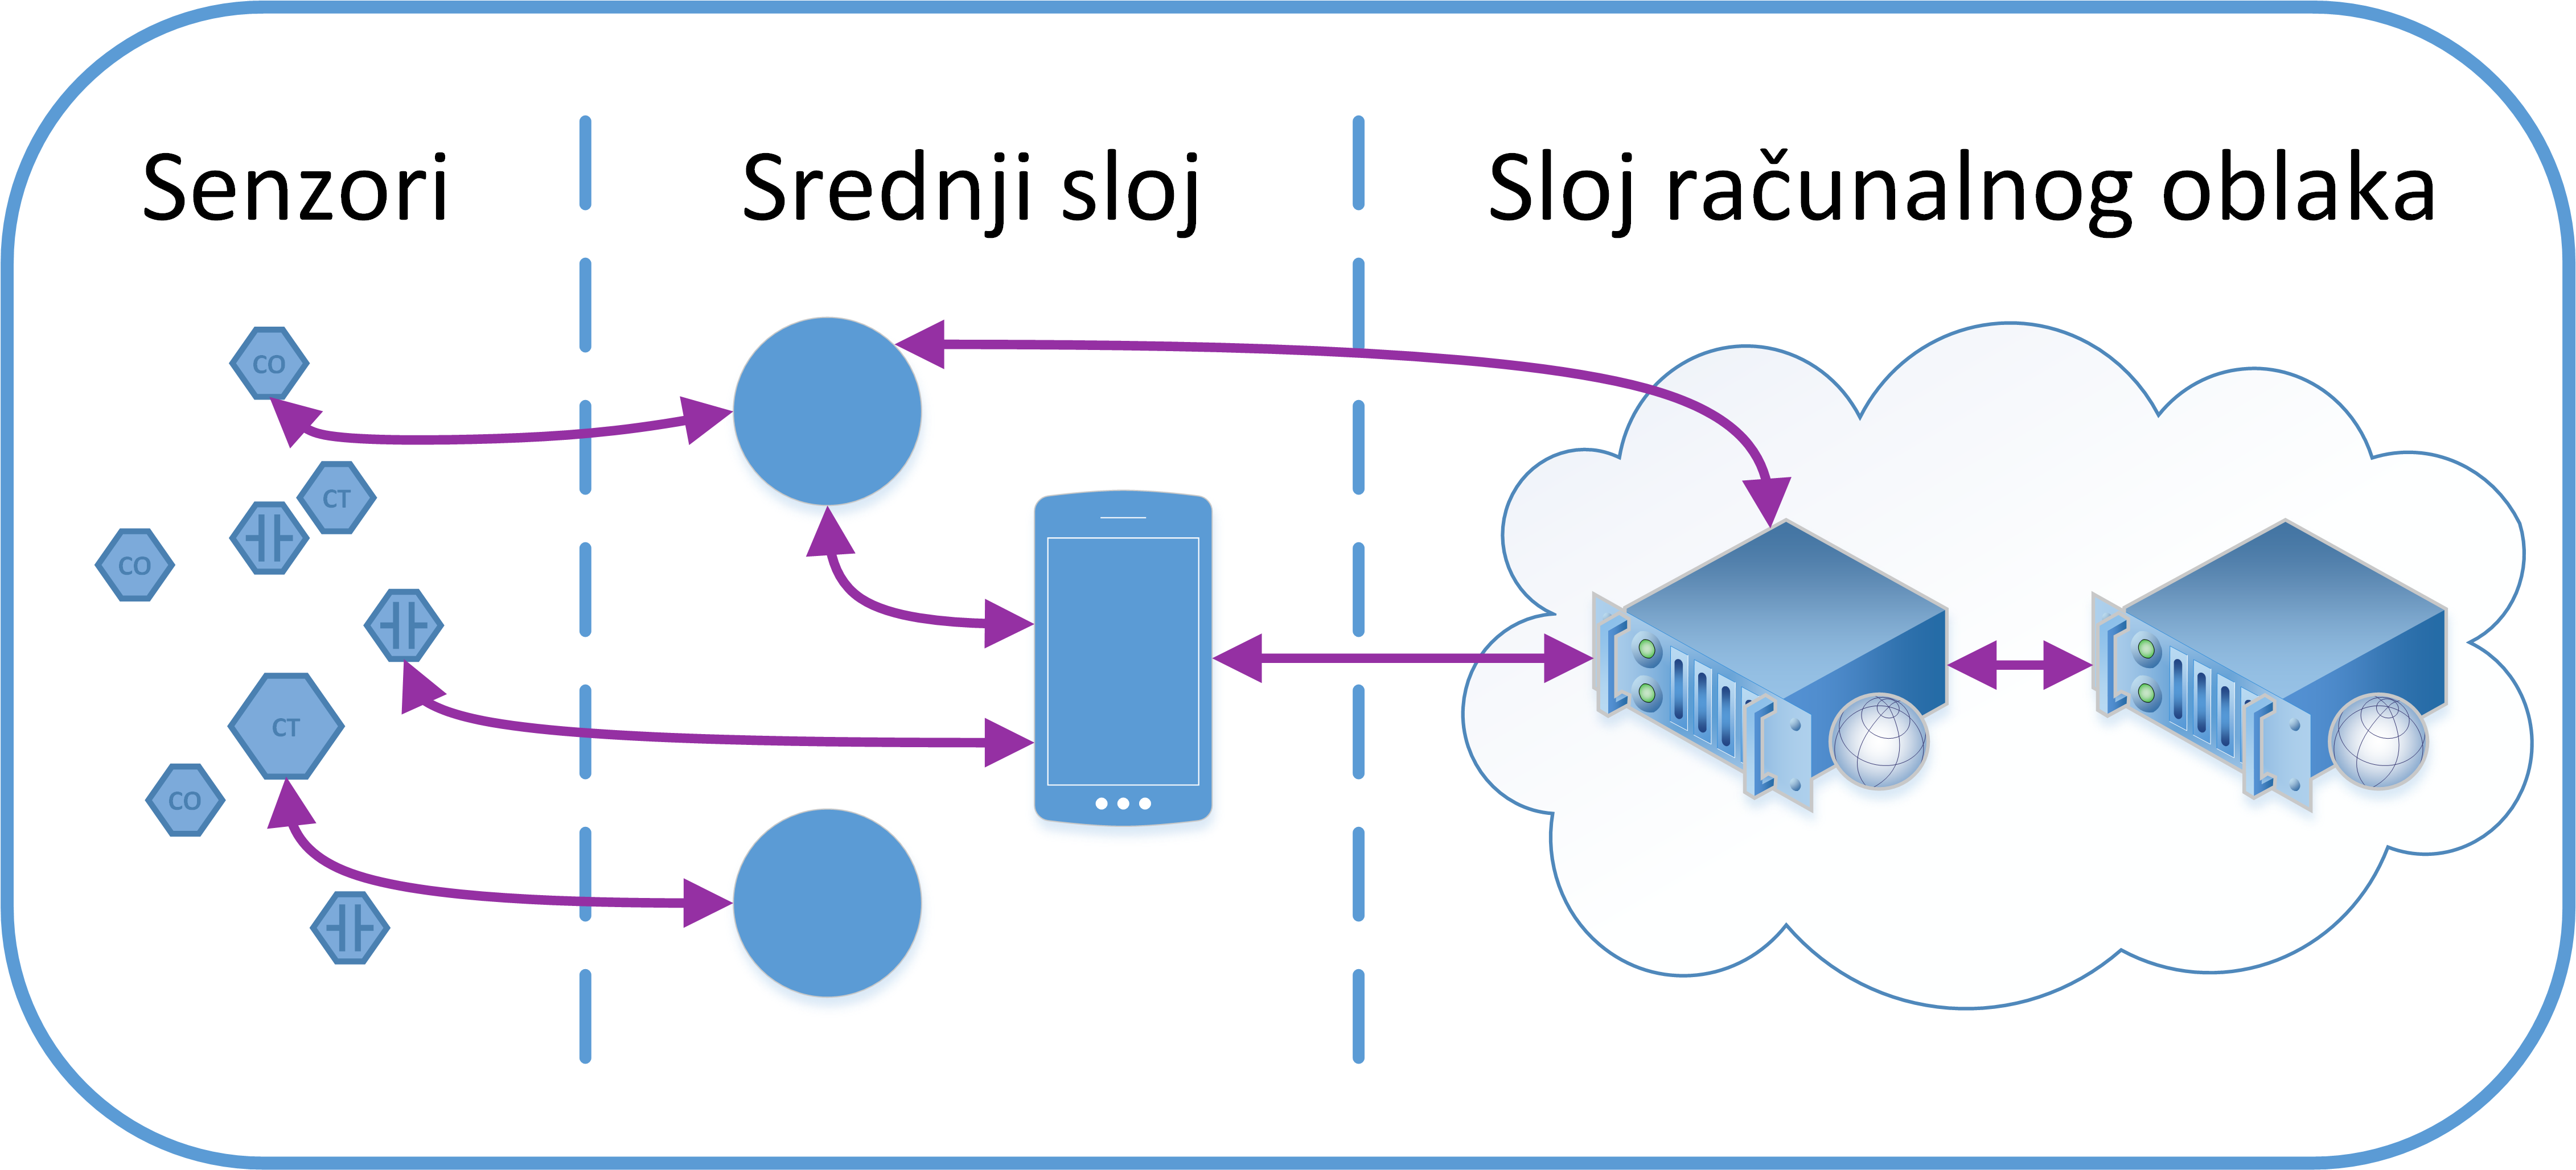
\includegraphics[width=0.6\textwidth]{iot_independent}
    \caption{Slojevita arhitektura Interneta stvari}
    \label{fig:iot1}
\end{figure}

U radu \cite{Kapadia:2009:opportunistic} prepoznati su sigurnosni
zahtjevi za okolinu Interneta stvari. Prilagodljiva sigurna
komunikacija omogućuje rješavanje problema zaštite podataka na različitim
slojevima arhitekture Interneta stvari \cite{zhang:2011:architecture}. Uz to
prepoznaje se i važnost manje zahtjevnih načina zaštite podataka za uređaje
senzorskog sloja \cite{Suo} kako bi se povećao broj sigurnih mjerenja tih
uređaja. 

% vim: spell spelllang=hr

\chapter{Protokol za sigurno dogovaranje kriptografskih algoritama}
\label{ch:model}

U ovom poglavlju opisan je novi protokol za sigurno dogovaranje
kriptografskih algoritama neovisan o komunikacijskom sloju, u daljnjem tekstu
ACAP (engl. \emph{Agile Cryptographic Agreement Protocol}). 
Osnovni zahtjevi na dizajn protokola ACAP su sljedeći:
\begin{itemize}
    \item sigurna razmjena kriptografskih ključeva,
    \item prilagodljivi dogovor kriptografskih algoritama,
    \item jednostavna arhitektura koja omogućava formalnu verifikaciju,
    \item neovisnost o komunikacijskom sloju i uređaju i
    \item učinkovita komunikacija s malim brojem poruka.
\end{itemize}

Protokol služi za komunikaciju između dvije strane (klijenta i poslužitelja) i
omogućava sigurno dogovaranje svih potrebnih preduvjeta kako bi se ostvarila buduća
sigurna komunikacija između te dvije strane gdje je klijent strana koja
započinje komunikaciju, a poslužitelj druga strana koja očekuje poruku za
početak dogovora. Protokol ACAP omogućuje i dogovor u sklopu paradigme
ravnopravnih čvorova gdje su svi čvorovi istovremeno klijenti i poslužitelji.

Nakon uspješne razmjene poruka obje strane imaju pristup sljedećim
podacima:
\begin{itemize}
    \item Tajnom ključu koji se generira iz zajedničke tajne koja se uspostavlja
	korištenjem protokola Diffie-Hellman \cite{DH}
	i omogućava uspostavljanje principa PFS (engl. \emph{Perfect Forward
	Secrecy}) \cite{krawczyk2011perfect}. Princip PFS omogućava tajnost
	razmjene podataka i u slučaju da se otkrije dugoročna zajednička tajna.
    \item Javnim ključevima koji se koriste za autentifikaciju komunicirajućih
	strana.
    \item Popisu kriptografskih algoritama koji su podržani na obje
	komunicirajuće strane te koji će se koristiti za ostvarivanje potrebnih
	sigurnosnih zahtjeva.
\end{itemize}

Na početku potpoglavlja \ref{sec:oznac} dan je pregled označavanja za sve
kriptografske operacije
koje se koriste za opis protokola. Potom slijedi opis poruka i razmjene poruka s
kojima se ostvaruje komunikacija u protokolu ACAP. Na kraju poglavlja
analizira se sigurnost predloženog protokola i opisuju se sigurnosni mehanizmi
koji su integrirani u protokol.

Protokol ACAP temeljen je na principu \emph{sign-and-mac} (SIGMA) koji je
opisan u poglavlju \ref{sec:sigma}. SIGMA kombinira razmjenu
ključa korištenjem Diffie-Hellman algoritma, digitalni potpis i algoritam HMAC
za zaštitu dogovora tako da
onemogućuje napadača da uspostavi napad čovjek u sredini. Protokol JFK, koji
je opisan u potpoglavlju \ref{sec:jfk}, također koristi princip SIGMA, što
objašnjava sličnost prve dvije poruke protokola ACAP s ovim protokolom. Dogovor
algoritama koji će se koristiti za osiguravanje komunikacije sličan je onom
koji je definiran u transportnom dijelu protokola SSH.

\section{Označavanje kriptografskih operacija}
\label{sec:oznac}

Za opis protokola koristi se standardni način označavanja kriptografskih
operacija. Oznaka $X$
predstavlja jednu stranu u komunikaciji, a oznaka $x$ predstavlja tajnu
komponentu Diffie-Hellman razmjene na odgovarajućoj strani. Klijent se označava
oznakom $I$ (od
engl. \emph{initiator}, započinjatelj), a poslužitelj oznakom $R$ (od
engl. \emph{responder}, odgovaratelj):

{
\renewcommand{\arraystretch}{1.40}
\begin{tabular}{p{1.0cm} p{13.5cm}}
$g^x	$ & javni dio Diffie-Hellman (DH) razmjene ključeva, uz specifikaciju DH
	    grupe koja se želi koristiti za komunikaciju, \\

$N_X	$ & jedinstvena privremena vrijednost (engl. \emph{nonce}) koja se koristi za
	    jedan dogovor, \\

$K	$ & ključ sjednice, rezultat je KDF operacije nad dijeljenom
	    tajnom (dijeljena tajna se računa iz $(g^x, y)$ ili $(g^y, x)$,
	    ovisno o komunikacijskoj strani, gdje su $x$ i $y$ tajni dijelovi
	    DH razmjene) i \emph{nonce} vrijednosti obje strane,

	    $K = KDF (g^{xy},N_I,N_R) $, \\

$PK_X	$ & javni ključ (ili digitalni certifikat), \\

$S_X\{\}$ & digitalni potpis s tajnim (privatnim) ključem koji se može
	    provjeriti s odgovarajućim javnim ključem $PK_X$,\\

$H_K\{\}$ & HMAC operacija uz korištenje ključa sjednice K, \\

$L_X	$ & popis podržanih kriptografskih algoritama, podijeljen u kategorije, \\

$L_{IR} $ & dogovoreni kriptografski algoritmi između klijenta ($I$) i poslužitelja ($R$)
	    tijekom ACAP razmjene, \\

$K_{IR} $ & tajni ključ koji je dogovoren između klijenta ($I$) i poslužitelja
	    ($R$), \\

$E_X	$ & poruka koja sadrži podatke o grešci koja se dogodila tijekom
	    komunikacije (koristi se samo u porukama ABORT). \\
\end{tabular}
}

\section{Poruke i tok komunikacije}
\label{sec:poruke}

Standardni tok komunikacije u protokolu ACAP prikazan je na
slici~\ref{msc}. U njemu je prikazano računanje i distribucija svih parametara
koji su potrebni za sigurnu komunikaciju.

\begin{figure}[ht]
\setlength{\instdist}{2.5cm}
\begin{centering}
\begin{msc}[c]{Protokol ACAP}
\declinst{c}{}{Klijent (I)}
\declinst{s}{}{Poslužitelj (R)}

\action*{generiranje $g^i,N_I$}{c}
\nextlevel[2]

\mess{\initi}{c}{s}
\mscmark[br]{$g^i,N_I$}{s}
\nextlevel[2]
\action*{generiranje $g^r,N_R$}{s}
\nextlevel[2]

\action*{$K=KDF(g^{ir},N_I,N_R)$}{s}
\nextlevel[3]

\mess{\initr}{s}{c}
\mscmark[bl]{$g^r,N_R,PK_R$}{c}
\nextlevel[2]

\action*{$K=KDF(g^{ri},N_I,N_R)$}{c}
\nextlevel[3]

\mess{\listi}{c}{s}
\mscmark[br]{$PK_I,L_I$ $$}{s}
\nextlevel[2]

\mess{\listr}{s}{c}
\mscmark[bl]{$L_R$}{c}
\nextlevel[2]

\referencestart{p}{\\$L_{IR},PK_I,PK_R,K_{IR}$}{c}{s}
\nextlevel[3]
\referenceend{p}

\end{msc}
\caption{Grafički prikaz razmjene poruka protokola ACAP}
\label{msc}
\end{centering}
\end{figure}


Protokol ACAP sastoji se od četiri osnovne poruke s pomoću kojih se izmjenjuju
javni ključevi, dogovara zajednička tajna te kriptografski algoritmi koji će se
koristiti za zaštitu daljnje komunikacije. 
Oznake u zagradama korištene u opisu poruka protokola označuju smjer poruke ($I
\rightarrow R$ označuje poruku koju klijent $I$ šalje poslužitelju $R$):

\begin{tabular}{p{3.0cm} p{8.0cm}}
    \initi($I \rightarrow R$): & $g^i, N_I$  \\
    \initr($R \rightarrow I$): & $g^r, N_R, PK_R, S_R\{g^r\}$,
    $H_K\{PK_R, N_I, N_R\}$ \\
    \listi($I \rightarrow R$): & $PK_I, L_I, S_I\{L_I,g^i,g^r\}$,
    $H_K\{PK_I, N_R, N_I\}$ \\
    \listr($R \rightarrow I$): & $L_R, S_R\{L_R,g^i,g^r,N_I,N_R\}$ \\
\end{tabular}
\vspace{5pt}

Klijent pokreće komunikaciju slanjem poruke \initi{}. Ona sadrži 
javni dio Diffie-Hellman razmjene klijenta ($g^i$) uz specifikaciju DH
grupe i klijentov
\emph{nonce} $N_I$. Ako poslužitelj podržava predloženu grupu odgovara
klijentu s porukom \initr{}.

Poruka \initr{} sadrži javni dio DH razmjene poslužitelja $g^r$, javni ključ
$PK_R$ poslužitelja i \emph{nonce} $N_R$. Poruka je zaštićena s pomoću digitalnog
potpisa javnog dijela DH razmjene $S_R\{g^r\}$ i HMAC-a javnog ključa i obje
privremene jedinstvene vrijednosti s ključem sjednice $K$ koji je uspostavljen
kroz DH, $H_K\{PK_R, N_I, N_R\}$.

\listi{} sadrži klijentov javni ključ $PK_I$ i popis podržanih
algoritama $L_I$. Digitalni potpis u $S_I\{L_I,g^i,g^r\}$ štiti popis podržanih
algoritama dok HMAC, koristeći ključ sjednice $K$, štiti klijentov javni ključ
$H_K\{PK_I, N_R, N_I\}$. Zadnja poruka u razmjeni je \listr{}. U toj
poruci prenosi se lista podržanih protokola poslužitelja $L_R$, koja je
zaštićena s digitalnim potpisom $S_R\{g^i,g^r,N_I,N_R,L_R\}$.

Nakon razmjene, klijent i poslužitelj imaju pristup popisu dogovorenih
algoritama $L_{IR}$, međusobnim javnim ključevima i zajedničkoj tajni $K_{IR}$
(poznatoj samo klijentu i poslužitelju).

\subsection{Rukovanje iznimkama}

Tijekom komunikacije moguće su iznimke koje će prouzročiti prekid izmjena
poruka. To je moguće u sljedećim slučajevima:
\begin{itemize}
\item različite Diffie-Hellman grupe u početnoj razmjeni,
\item pogrešan zaštitni sažetak HMAC,
\item pogrešan digitalni potpis ili
\item nepostojanje zajedničkih algoritama za korištenje kod klijenta i
poslužitelja.
\end{itemize}

U svrhu rukovanja iznimkama definiramo poruke ABORT koje su različite za
klijenta i poslužitelja:

\begin{tabular}{p{3.4cm} p{8.0cm}}
    \abortr($R \rightarrow I$): & $E_R, N_I, PK_R, S_R\{N_I, E_R\}$ \\
    \aborti($I \rightarrow R$): & $E_I, N_R, PK_I, S_I\{N_R, E_I\}$ \\
\end{tabular}
\vspace{5pt}

ABORT poruke sadrže kratak opis greške, odgovarajući \emph{nonce}, javni
ključ te digitalni potpis \emph{noncea} i opisa greške.

\section{Kriptografski algoritmi i ključevi za dogovaranje}

Kako bi komunicirajuće strane mogle na siguran način dogovoriti kriptografske
algoritme i ključeve potrebne za zaštitu komunikacije, obje strane u
komunikaciji moraju podržavati nekoliko osnovnih vrsta kriptografskih algoritama
za provedbu dogovora:
\begin{itemize}
    \item postupak razmjene ključeva Diffie-Hellman za dobivanje zajedničke
	tajne $g^{ir}$,
    \item operacija KDF za izračunavanje ključa sjednice $K$ i tajne za zaštitu
	naknadne komunikacije $K_{IR}$ iz zajedničke tajne dobivene DH postupkom
	i \emph{nonceva} $N_I$ i $N_R$,
    \item funkcija kriptografskog sažetka za izračun HMAC operacija s
	ključem sjednice $K$ i
    \item asimetrični algoritam za izračun i provjeru digitalnih potpisa tijekom
	dogovora.
\end{itemize}

Da bi se ostvario dogovor više različitih vrsta asimetričnih algoritama za zaštitu
komunikacije nužno je razmijeniti javne ključeve za sve podržane
asimetrične algoritme i na kraju odabrati ključ koji odgovara dogovorenom
asimetričnom algoritmu.

Za zaštitu komunikacije u prototipu protokola koriste se sljedeći algoritmi:
Diffie-Hellman 1024 MODP grupa \cite{rfc5114}, KDF operacija zasnovana na HMAC
inačici SHA-256 funkcije kriptografskog sažetka (HKDF \cite{rfc5869}), SHA-256
kriptografski sažetak za HMAC operacije i RSA-1536 kao asimetrični algoritam za
digitalne potpise. Uz te algoritme može se koristiti Diffie-Hellman
algoritam zasnovan na eliptičnim krivuljama, kao i ECDSA algoritam za digitalni
potpis (oba algoritma koriste ključeve veličine 256 bita).

\section{Dogovor kriptografskih algoritama}
\label{sec:dogovor}

Popisi podržanih kriptografskih algoritma podijeljeni su u kategorije. Te
kategorije se mogu definirati prema trenutnim potrebama zaštite. Za zapis
popisa koristi se format JSON~\cite{rfc4627}.
Na slici~\ref{fig:alg_list} vidi se primjer s više različitih kategorija i
skupova kriptografskih algoritama.
\begin{figure}[htb]
\begin{small}
\begin{verbatim}
{
    "hash":["SHA-256", "RIPEMD", "SHA-1", "MD5"],
    "secret_key":["AES-CTR_256", "AES-CBC_128", "3DES_192"],
    "public_key":["ECDSA_192", "DSA_2048", "RSA_2048"],
    "cryptographic_suite":[
      "TLS_ECDH_ECDSA_WITH_AES_128_GCM_SHA256",
      "TLS_DHE_PSK_WITH_AES_128_CBC_SHA256",
      "TLS_RSA_WITH_RC4_128_SHA" ]
}
\end{verbatim}
\end{small}
\vspace{-15pt}
\caption{Popisi kriptografskih algoritama i skupova koji se dogovaraju}
\label{fig:alg_list}
\end{figure}


Za dogovor kriptografskih algoritama u programskom ostvarenju koriste se principi iz
protokola SSH \cite{rfc4253}. Ovisno o
namjeni i okruženju u kojem se koristi protokol, moguće je definirati drukčije
algoritme dogovora koji će uzimati dodatne parametre prilikom odluke.
Prilagodba algoritma za dogovor za korištenje u okolini Interneta Stvari
prikazana je u poglavlju \ref{ch:iot}.

Kriptografski algoritmi odabiru se zasebno za svaku vrstu
algoritma: sažetak (\texttt{hash}), kriptografija tajnog ključa
(\texttt{secret\_key}), kriptografija javnog ključa (\texttt{public\_key}) ili
korištenjem skupa kriptografskih algoritama (\texttt{cryptographic suite}). Uz
to, moguć je i dogovor drugih parametara sigurne komunikacije, kao što je način
generiranja tajnih ključeva iz dobivene zajedničke tajne.
U popisu algoritama za kriptografiju javnog i tajnog ključa zadnji dio u imenu
algoritma predstavlja duljinu ključa koji je podržan, npr.
\texttt{AES-CTR\_256} predstavlja algoritam AES koji koristi CTR način
ulančavanja blokova s tajnim ključem duljine 256 bita.

Odabire se prvi algoritam s popisa klijenta koji se ujedno nalazi na popisu
poslužitelja. Primjer dogovora algoritama između klijenta i poslužitelja
prikazan je slikom \ref{fig:neg_lists}. Preduvjet je da svi algoritmi budu
poredani prema sigurnosti algoritma i duljini ključa. Algoritmi mogu biti poredani
i prema zahtjevnosti izračunavanja ukoliko se radi o okruženju s ograničenim
računalnim resursima. Prošireni model dogovora kriptografskih algoritama
za okolinu Interneta stvari prikazan je u poglavlju \ref{sec:iotprilag}.

\begin{figure}
\begin{subfigure}{0.33\linewidth}
\begin{framed}
\begin{small}
\begin{verbatim}
"hash":[
    "SHA-256",
    "RIPEMD",
    "SHA-1"],
"secret_key":[
    "AES-CTR_256",
    "AES-CBC_128",
    "3DES_192"],
"public_key":[
    "RSA_1024",
    "RSA_2048",
    "ECDSA_192"]
\end{verbatim}
\vspace{-15pt}
\end{small}
\end{framed}
\vspace{-10pt}
\caption{Popis algoritama klijenta}
\end{subfigure}
\begin{subfigure}{0.32\linewidth}
\begin{framed}
\begin{small}
\begin{verbatim}
"hash":[
    "SHA3-512",
    "SHA-512",
    "SHA-256"],
"secret_key":[
    "AES-CTR_256",
    "Salsa20_256",
    "AES-CBC_128"],
"public_key":[
    "ECDSA_224",
    "ECDSA_192",
    "RSA_2048"]
\end{verbatim}
\vspace{-15pt}
\end{small}
\end{framed}
\vspace{-10pt}
\caption{Popis algoritama poslužitelja}
\end{subfigure}
\begin{subfigure}{0.33\linewidth}
\begin{framed}
\begin{small}
\begin{verbatim}
"hash":
    "SHA-256",


"secret_key":
    "AES-CTR_256",


"public_key":
    "RSA_2048"


\end{verbatim}
\vspace{-15pt}
\end{small}
\end{framed}
\vspace{-10pt}
\caption{Dogovoreni popis algoritama}
\end{subfigure}
\caption{Primjer ponuđenih i dogovorenih algoritama}
\label{fig:neg_lists}
\end{figure}

Popisi preporuka za korištenje određenih algoritama redovito se izdaju od strane
savjetodavnih agencija za pojedine države i zajednice. Te se preporuke mogu
pronaći na web sjedištu tvrtke BlueKrypt~\footnote{BlueKrypt -- Keylength --
Cryptographic Key Length Recommendation -- \url{http://www.keylength.com/en/}}.

Protokol ACAP ne podržava mogućnost ponovne razmjene popisa
podržanih algoritama, već je potrebno ponoviti cijeli postupak dogovora kako bi
se algoritmi i ključevi osvježili i prilagodili trenutnom stanju komunicirajućih
strana. Nakon uspješnog dogovora ključeva i algoritama, aplikacija
koja se koristi protokolom definira trajanje dogovorenih parametara.
Preporučeni interval dogovora parametara je jedan sat, što je uobičajena
vrijednost trajanja IPsec \emph{Security Association} dogovora
\footnote{Trenutno strongSwan IPsec rješenje koristi preporučeni interval
od jednog sata: \\
\url{https://wiki.strongswan.org/projects/strongswan/wiki/ExpiryRekey}, dok je to kod
Cisco opreme interval od 24 sata:
\url{http://www.cisco.com/c/en/us/td/docs/security/asa/asa95/configuration/vpn/asa-95-vpn-config.pdf}}.
Taj interval može se prilagoditi ovisno o okruženju u kojem se koristi
protokol ACAP.

\section{Analiza sigurnosti i mehanizama protokola ACAP}
\label{sec:sigurnost}

Cilj protokola ACAP je omogućavanje jednostavne integracije i formalne
verifikacije kako bi se mogla jamčiti sigurna komunikacija. Zbog toga je
donekle ograničena količina funkcionalnosti kako bi se smanjila vjerojatnost
pojavljivanja napada na protokol i njegovo programsko ostvarenje.
Jedna od namjerno izostavljenih
funkcionalnosti je podrška za ponovno dogovaranje koje se nastavlja na
prethodni dogovor.  Jedino što se pamti od početnog dogovora su javni ključevi
obje komunicirajuće strane.

Poruke u protokolu sadrže samo podatke koji su nužni da bi se zaštitio dogovor
algoritama i ključeva. Kako bi se spriječili napadi ponavljanjem poruka, u svaku
poruku su uključene \emph{nonce} vrijednosti i javni dijelovi DH
razmjene. U porukama gdje nisu eksplicitno uključene one se koriste za izračun
digitalnih potpisa i HMAC sažetaka.

Princip SIGMA \cite{Krawczyk2003sigma} koristi se za sprječavanje napada
čovjek u sredini jer implicitno povezuje ključ sjednice $K$ (koji je dobiven
iz zajedničke tajne uspostavljene kroz DH razmjenu korištenjem funkcije KDF) s
javnim ključevima komunicirajućih strana $PK_I$ i $PK_R$.

Pregled sigurnosnih mehanizama i razine na kojoj se ostvaruju prikazana je u
tablici \ref{tab:zahtjevi}. Sigurnosni mehanizmi ostvareni na razini
programskog ostvarenja dodatno su objašnjeni u poglavlju \ref{ch:impl}.

\begin{table*}[hbt]
\caption{Pregled sigurnosnih mehanizama protokola ACAP}
\renewcommand{\arraystretch}{1.3}
\label{tab:zahtjevi}
\centering
\small
\begin{tabular}{p{6.4cm} p{3.0cm} p{5.0cm} }
\hline
Sigurnosni mehanizam
    & Razina rješenja
    & Način ostvarivanja
    \\ \hline \hline
Djelomični nedostatak dogovora\newline algoritma u ACAP razmjeni
    & dizajn protokola
    & mali utjecaj i mogućnost\newline dvostrukog dogovora
    \\ \hline
Računalna neovisnost tajnih ključeva
    & ostvarenje
    & ugrađen mehanizam za neovisno izračunavanje ključeva
    \\ \hline
Smanjenje utjecaja DoS napada
    & ostvarenje
    & najzahtjevniji izračuni odvojeni u pozadinski proces
    \\ \hline
Uspostavljanje povjerenja\newline komunicirajućih strana
    & dizajn protokola
    & na razini postojećih rješenja
    \\ \hline
Sprječavanje napada čovjek u sredini
    & dizajn protokola
    & verificirano u sklopu\newline formalne verifikacije
    \\ \hline
Sprječavanje napada ponavljanjem\newline poruka
    & dizajn protokola\newline i ostvarenje
    & verificirano u sklopu\newline formalne verifikacije
    \\ \hline
\end{tabular}
\end{table*}

\subsection{Djelomični nedostatak dogovora algoritama u ACAP razmjeni}
Cjelokupna razmjena sastoji se od samo četiri poruke te se uvijek radi sa svježim
\emph{nonce} vrijednostima. U slučaju da jedan od kriptografskih algoritama
koji se koristi
za razmjenu postane ranjiv, zbog malog broja poruka ne bi bilo moguće
ozbiljno ugroziti razmjenu u sklopu protokola ACAP. Zbog toga se na početku
razmjene izmjenjuje isključivo informacija o Diffie-Hellman grupi kako bi se
osiguralo dogovaranje s trenutno najboljim DH parametrima i dobila zajednička
tajna dovoljne veličine. Trenutno programsko ostvarenje protokola ACAP koristi
najnovije sigurne kriptografske algoritme, kao što su SHA-256
sažetak za HMAC izračune i kriptografija temeljena na eliptičnim krivuljama za
algoritme asimetričnog kriptosustava (DH i digitalno potpisivanje). Važno je
napomenuti da bi uvođenje jednostavnog načina dogovora algoritama za početni
dogovor zahtijevalo još barem jednu poruku na početku komunikacije i
omogućilo više točaka napada. U tom slučaju napadač bi mogao utjecati na razinu
sigurnosti tako da se koristi najslabiji trenutno podržani kriptografski
algoritam. Najbolji način izvedbe dogovora algoritma za provedbu protokola ACAP
je dvostruko korištenje protokola: jednom za dogovor algoritama za razmjenu, a
potom dogovor s novim algoritmima za konačni rezultat.

\subsection{Računalna neovisnost tajnih ključeva}
\label{sec:keys}
Ključni dio principa SIGMA leži u
računalnoj neovisnosti zajedničkih tajni koje se koriste za razmjene poruka. To
se odnosi na ključ sjednice $K$ i tajni ključ koji je rezultat cjelokupne
razmjene. Oba ključa izračunavaju se iz iste zajedničke tajne, uz uvjet da jedan
ključ ne otkriva nikakve podatke o drugom ključu, kako je opisano u
dodatku članka \cite{Krawczyk2003sigma}. Nakon što se završi razmjena protokola
ACAP, komunicirajuće strane dobivaju tajni ključ odgovarajuće duljine
za odabrani algoritam šifriranja  tijekom dogovora koji je računalno neovisan od
tajne koja je dogovorena putem protokola Diffie-Hellman. Kod programskog
ostvarenja protokola važno je da je zajednička tajna
dostupna samo u radnoj memoriji za vrijeme izvođenja dogovora i briše se odmah
nakon
razmjene kako bi se spriječilo otkrivanje podataka o tajni. U protokolu ACAP
računalna neovisnost izvedena je pravilnim korištenjem funkcije KDF za
dobivanjem računalno neovisnih ključeva.

\subsection{Smanjenje utjecaja DoS napada}
\label{sec:dos}
Napadi uskraćivanja usluge (engl.
\emph{Denial of Service, DoS attacks}) imaju za cilj iscrpiti resurse koji su na
raspolaganju određenoj usluzi kako bi se onemogućio pristup toj usluzi, što se
najčešće postiže slanjem velikog broja poruka na određenu uslugu.

Da bi 
poslužitelj stvorio poruku \initr{}, kao odgovor na poruku \initi{}, mora
odraditi
vremenski zahtjevnu operaciju generiranja nasumičnog broja pogodnog za
Diffie-Hellman razmjenu zajedno s izračunom ključa sjednice $K$ te izračunom
digitalnog potpisa i HMAC sažetka. To je računalno najzahtjevnija operacija
cjelokupne razmjene i predstavlja moguću točku napada na protokol.
Napadač bi mogao proizvesti ogromnu količinu lažnih \initi{} poruka koje bi
uzrokovale nedostatak resursa na strani poslužitelja.
Utjecaj takvog napada smanjuje se korištenjem Diffie-Hellman tajne tijekom
kratkog vremenskog perioda i prethodnim izračunom računalno zahtjevnijeg dijela
\initr{} poruke ($g^r, S_R\{g^r\}$). Generiranje zahtjevnijeg dijela poruke u
tom se slučaju obavlja kao pozadinska procedura u sklopu ACAP poslužitelja. Stoga
su jedine operacije koje poslužitelj mora
odraditi prilikom primitka poruke \initr{} izračun ključa sjednice
$K$ i izračun HMAC sažetka s tim ključem ($H_K\{PK_R, N_I, N_R\}$). Sličan
mehanizam koristi se u protokolu JFK \cite{aiello2004jfk}.

\no{
\begin{figure}[ht]
\setlength{\instdist}{4cm}
\begin{centering}
    \begin{msc}[c]{Razmjena \initi{} i \initr{} poruka}
\declinst{c}{}{Klijent (I)}
\declinst{s}{}{Poslužitelj (R)}

\mess{gen $g^r, N_R, S_R(g^{r})$}{s}{s}

\action*{generiranje $g^i,N_I$}{c}
\nextlevel[4]

\mess{$g^i, N_I$}{c}{s}
\nextlevel[1]

\action*{$K=KDF(g^{ir},N_I,N_R)$}{s}
\nextlevel[4]

\mess{$\mathbf{g^r}, \mathbf{N_R}, PK_R, \mathbf{S_R(g^r)}, H_K\{...\}$}{s}{c}

\end{msc}
\caption{Smanjenje utjecaja DoS napada}
\label{msc_dos}
\end{centering}
\end{figure}
}

\subsection{Uspostavljanje povjerenja između komunicirajućih strana}
Uspostavljanje povjerenja (engl. \emph{trust establishment}) između dvije
komunicirajuće strane predstavlja mogućnost da se na određeni način provjeri da
svakoj od komunicirajućih strana pripada adresa s pomoću koje komunicira. To
se u sklopu suvremenih računalnih sustava ostvaruje s pomoću infrastrukture
javnog ključa (engl. \emph{Public Key Infrastructure}, PKI) ili ranijom
distribucijom identifikacijskih podataka. Na taj se način stvara početno
povjerenje (engl. \emph{root of trust}) na kojem se temelji sva buduća
komunikacija.

Protokol ACAP
ne postavlja ograničenja na razmjenu identifikacijskih podataka. Mogu se
razmjenjivati samostalni javni ključevi kao i digitalno potpisani javni ključevi
u obliku certifikata. To ne zahtijeva nikakvu promjenu u porukama \initr{} i
\listi{}. U slučaju korištenja digitalno potpisanih certifikata aplikacija koja
koristi ACAP mogla bi provjeravati valjanost certifikata kako bi se osiguralo
povjerenje između komunicirajućih strana. To omogućava jednaku razinu sigurnosti
kao u protokolima SSL/TLS i IPsec te zahtijeva istu infrastrukturu javnog
ključa koja se trenutno koristi za
osiguravanje povjerenja. Ako se ne koristi PKI, onda je potrebno
odraditi prvu razmjenu protokola u kontroliranim uvjetima kako bi se zapamtili
javni ključevi i ostvarilo početno povjerenje između komunicirajućih strana. Uz
to, javne ključeve je moguće distribuirati drugim kanalom prije početne
razmjene.

\subsection{Sprječavanje napada čovjek u sredini}
U scenariju napada čovjek u
sredini napadač se klijentu u komunikaciji predstavlja kao poslužitelj i
obratno. Pretpostavka protokola ACAP je da se dogovoreni tajni ključ i algoritmi
vežu s javnim ključevima s kojima su ti parametri dogovoreni. Cilj je
onemogućiti napadača da se predstavlja kao vlasnik klijentskog odnosno
poslužiteljskog privatnog ključa, što izravno onemogućuje napadača da utječe na
dogovorene kriptografske algoritme i zajedničku tajnu u slučaju prethodno
uspostavljenog početnog povjerenja.

Pretpostavimo da
napadač pokuša promijeniti poruke u razmjeni kako bi došao do tajnog ključa koji
će dvije strane koristiti za komuniciranje. Ako napadač promijeni poruku \initi{}
($g^i,N_I$) tako da uvede drukčiji DH nasumični broj (npr. $i'$ i
izračunati $g^{i'}$),
mogao bi također izračunati povratnu \initr{} poruku korištenjem drugog para
privatnog i javnog ključa. Uz to bi morao generirati još jedan DH nasumični broj
(npr. $r'$ i izračunati $g^{r'}$) i tada bi poruka \initr{} 
bila oblika ($g^{r'}, N_R, PK_{R'}, S_{R'}\{g^{r'}\},
H_{K'}\{PK_{R'}, N_I, N_R\}$). To bi isto tako vodilo i do promjene ključa
sjednice $K$ u ključ $K'$. Sva naknadna komunikacija nakon te dvije početne
poruke bila bi neuspješna zbog provjere HMAC sažetaka i komunicirajuće strane ne
bi mogle provesti dogovor niti povezati javne ključeve s dogovorenim
kriptografskim algoritmima i promijenjenom zajedničkom tajnom. Dodatno,
otpornost na napade čovjek u sredini dokazana je postupkom formalne
verifikacije koji je prikazan u poglavlju \ref{sec:verif}.

\subsection{Sprječavanje napada ponavljanjem poruka}
\label{sec:replay}
U slučaju sprječavanja napada ponavljanjem poruka cilj napadača
je u jednom trenutku spremiti cjelokupnu razmjenu poruka u dogovoru i kasnije
odraditi identičnu razmjenu poruka kako bi komunicirajuće strane koristile
stariji ključ i kriptografske algoritme. Ovakav napad bi omogućio da se svaki
dogovor poništi tako da se ponovi stariji spremljeni dogovor.

U trenutku kad napadač šalje prethodno zabilježenu poruku, poslužitelj ima novu
vrijednost \emph{noncea} $N_R$. To znači da bi nova vrijednost trebala biti
korištena za izračun HMAC sažetka ($H_K\{PK_I, N_R, N_I\}$) koji je sadržan u
poruci \listi{}. To nije moguće odraditi u pasivnom scenariju slanja prethodno
zabilježenih poruka. U slučaju aktivnog napada napadač bi trebao biti u
mogućnosti promijeniti zabilježene poruke, što je onemogućeno promjenom
Diffie-Hellman vrijednosti za kasnije razmjene. Shodno tome sve provjere HMAC
sažetaka bile bi negativne.

\section{Usporedba protokola ACAP s protokolom za upravljanje prijenosom
podataka u protokolu SSH}

Za dogovor algoritama i ključeva u protokolu za upravljanjem prijenosom podataka
protokola SSH potrebno je šest poruka.
Prve dvije poruke (KEXINIT\textsubscript{C} i
KEXINIT\textsubscript{S}) služe za razmjenu i dogovor algoritama koji će se
koristiti za dogovor ključeva. Dogovaraju se algoritmi za Diffie-Hellman (DH)
razmjenu, algoritmi simetričnog kriptosustava i algoritmi za stvaranje zaštitnog
sažetka HMAC. Nakon dogovora algoritma razmjenjuju se poruke za dogovor
DH zajedničke tajne (KEXDH\_INIT i KEXDH\_REPLY). Poruka KEXDH\_REPLY također
sadrži javni ključ poslužitelja i digitalni potpis razmjene s kojim se
provjerava vjerodostojnost dosadašnje razmjene. Na kraju se razmjenjuju
poruke za dogovor novih ključeva (NEWKEYS\textsubscript{C} i
NEWKEYS\textsubscript{S}) nakon kojih su uspostavljeni novi ključevi za zaštitu
komunikacije. Cjelokupna razmjena poruka prikazana je na slici \ref{msc_ssh}.
Razmjenu je moguće skratiti na pet poruka tako da se poruka
NEWKEYS\textsubscript{S} šalje zajedno s porukom KEXDH\_REPLY.


Protokol za upravljanje prijenosom podataka unutar SSH mogao bi se iskoristiti
za uslugu koju pruža protokol ACAP (dogovor kriptografskih algoritama i
ključeva), ali
pritom je važno uzeti u obzir razlike između ta dva protokola. Razlike protokola
za upravljanje prijenosom podataka u odnosu na protokol ACAP su sljedeće:
\begin{itemize}
    \item veći broj poruka u razmjeni,
    \item razmjena javnog ključa samo za poslužitelj,
    \item manji broj poruka s digitalnim potpisom,
    \item kasnije otkrivanje promjene poruka za dogovor algoritama i
    \item nemogućnost smanjivanja opterećenosti poslužitelja prilikom
	generiranja digitalnog potpisa razmjene.
\end{itemize}

\begin{figure}[ht]
\setlength{\instdist}{2.5cm}
\begin{centering}
\begin{msc}[c]{Protokol SSH za upravljanje prijenosom podataka}
\declinst{c}{}{SSH Klijent (C)}
\declinst{s}{}{SSH Poslužitelj (S)}

\mess{KEXINIT\textsubscript{C}}{c}{s}
\mscmark[br]{$L_C$}{s}
\nextlevel[2]

\mess{KEXINIT\textsubscript{S}}{s}{c}
\mscmark[bl]{$L_S$}{c}
\nextlevel[1.5]

\referencestart{p}{\\$L_{CS}$}{c}{s}
\nextlevel[2]
\referenceend{p}
\nextlevel[0.5]

\action*{generiranje $x, g^x$}{c}
\action*{generiranje $y, g^y$}{s}
\nextlevel[3]

\mess{KEXDH\_INIT}{c}{s}
\mscmark[br]{$g^x$}{s}
\nextlevel[1.5]

\action*{$K=g^{xy}$}{s}
\nextlevel[2]
\action*{$DP=S_S(C, S, KEXINIT_{(S,C)}, PK_S, K)$}{s}
\nextlevel[3.5]

\mess{KEXDH\_REPLY}{s}{c}
\mscmark[bl]{$PK_S,g^y$}{c}
\nextlevel[1.5]
\action*{$K=g^{xy}$}{c}
\nextlevel[2]

\mess{NEWKEYS\textsubscript{C}}{c}{s}
\nextlevel[2]

\mess{NEWKEYS\textsubscript{S}}{s}{c}
\nextlevel[1]

\referencestart{p}{\\$K_{CS}$}{c}{s}
\nextlevel[2]
\referenceend{p}

\end{msc}
\caption{Grafički prikaz razmjene poruka protokola za upravljanje prijenosom
    podataka protokola SSH}
\label{msc_ssh}
\end{centering}
\end{figure}


Kada bi se principi iz protokola za upravljanje prijenosom podataka primijenili
za uslugu koju pruža protokol ACAP tada bi za potpunu razmjenu trebala barem
jedna poruka više. Dodatni problem je što komunicirajuće strane nisu ravnopravne
već se razmjenjuje samo javni ključ poslužitelja i ne postoji autentifikacija
klijenta u sklopu protokola za upravljanje prijenosom podataka. Autentifikacija
klijenta se odrađuje u sklopu protokola za autentifikaciju korisnika protokola
SSH. Kako se digitalni potpis koristi samo kod slanja digitalnog potpisa
razmjene složenost kriptografskih operacija tijekom razmjene je niža nego kod
protokola ACAP, ali isto tako nije moguće autentificirati klijenta.

U slučaju napada čovjek u sredini promjenu početnih poruka KEXINIT bit će moguće
otkriti tek nakon primitka KEXDH\_REPLY poruke koja sadrži digitalni potpis
razmjene. U sklopu protokola ACAP promjenu poruke u razmjeni moguće je
prepoznati prije jer su sve poruke osim prve zaštićene zaštitnom sumom HMAC ili
digitalnim potpisom.  Konačno digitalni potpis razmjene sadrži podatke koje je
poslao klijent, te ga je potrebno generirati u trenutku kad poslužitelj primi i
poruku KEXINIT\textsubscript{C} i KEXDH\_INIT. 
Zbog toga je protokol SSH osjetljiviji na napad uskraćivanja usluge u odnosu na
ACAP.

% vim: spell spelllang=hr

\chapter{Formalna verifikacija modela}
\label{ch:verif}

Ispravnost protokola može se provjeriti formalnom verifikacijom modela protokola
uz zadane preduvjete koje model
mora zadovoljiti. Protokol ACAP je specificiran i formalno verificiran s pomoću
alata Scyther~\cite{cremers2007scyther}. Scyther omogućuje formalnu verifikaciju
modela protokola i sigurnosnih zahtjeva uz korištenje sigurnosnih
primitiva poput sažetaka, simetrične kriptografije i kriptografije javnog ključa.

\comment{dodati kratko poglavlje o načinu na koji scyther verificira protokole}

U ovom poglavlju pojašnjena je sintaksa za specifikaciju modela protokola i
specificiran je model protokola ACAP. U nastavku se prikazuje izvođenje
definiranog modela i analiziraju se rezultati verifikacije.

\section{Značajke jezika SPDL}

Alat Scyther za opis protokola koristi jezik SPDL (\emph{Security Protocol Definition
Language}). U tom jeziku moguće je koristiti sljedeće pojmove:
\begin{itemize}
\item Kriptografske funkcije za standardne kriptografske operacije:
    \begin{itemize}
	\item kriptografski sažetak (\texttt{hashfunction}), 
	\item simetrično šifriranje podataka (\texttt{\{secret\}key})
	\item asimetrično šifriranje podataka (\texttt{\{secret\}pk\{I\}} ili
	    \texttt{\{hash\}sk\{I\}}).
    \end{itemize}
\item Korisnički definirane konstante za definiciju jednosmjernih funkcija
    (\texttt{Function}), jedinstvenih privremenih vrijednosti
    (\texttt{Nonce}) i univerzalnih varijabli (\texttt{Ticket}).
\item Definiciju protokola (\texttt{protocol ime\_protokola}) koja obuhvaća
    uloge (\texttt{role}) komunicirajućih strana. U svakoj
    ulozi definiraju se varijable koje se koriste za komunikaciju zajedno s
    događajima slanja (\texttt{send}) i primanja (\texttt{recv}) poruka koji
    opisuju komunikaciju. Nakon opisa komunikacije slijede definicije
    sigurnosnih zahtjeva na protokol (\texttt{claim}) koje se provjeravaju
    prilikom verifikacije.
\end{itemize}

U idućem poglavlju dan je primjer formalne verifikacije jednostavnog protokola
za uzajamnu autentifikaciju.

\section{Primjer verifikacije jednostavnog protokola}

Za primjer modeliranja i verifikacije jednostavnog protokola odabran je protokol
Needham-Schroeder-Lowe (NSL)~\cite{lowe1996breaking}. Protokol NSL je popravljena
inačica Needham-Schroeder protokola čija je osnovna namjena uzajamna
autentifikacija dvije komunicirajuće strane. Razmjena poruka u protokolu NSL
prikazana je izrazima na slici \ref{fig:nsl_spec}, gdje I predstavlja započinjatelja
(engl. \emph{initiatior}), a R primatelja (engl. \emph{responder}),
$N_X$ su \emph{nonce} vrijednosti, $PK_X$ javni ključevi, dok su uloge $I$ i $R$
identiteti komunicirajućih strana (certifikati ili javni ključevi).

\begin{figure}[htb]
    \begin{center}
\begin{tabular}{p{1.5cm} p{3.0cm}}
    I $\rightarrow$ R: & $(I, N_I)_{PK_R}$\\
    R $\rightarrow$ I: & $(N_I,N_R,R)_{PK_I}$\\
    I $\rightarrow$ R: & $(N_R)_{PK_R}$\\
\end{tabular}
    \end{center}
\vspace{-15pt}
\caption{Opis protokola Needham-Schroeder-Lowe}
\label{fig:nsl_spec}
\end{figure}

U modelu protokola definiraju se dvije uloge: započinjatelj I i primatelj R.
Definicija dvije osnovne uloge protokola NSL prikazana je na slici
\ref{fig:nsl_def}. Uloga \texttt{I} predstavlja klijenta, odnosno započinjatelja
komunikacije (engl. \emph{initiator}), a uloga \texttt{R} predstavlja
poslužitelja, odnosno primatelja (engl. \emph{responder}).

\begin{figure}[htb]
\begin{subfigure}[t]{0.5\linewidth}
\begin{small}
\begin{verbatim}
protocol nsl(I, R) {

  # uloga započinjatelja
  role I { ... }

  # uloga primatelja
  role R { ... }
}
\end{verbatim}
\end{small}
\vspace{-5pt}
\subcaption{Definicija uloga}
\label{fig:nsl_def}
\end{subfigure}
\begin{subfigure}[t]{0.5\linewidth}
\begin{small}
\begin{verbatim}
 role I {
  fresh ni: Nonce; var nr: Nonce;

  send_1(I,R, {I,ni}pk(R));
  recv_2(R,I, {ni,nr,R}pk(I));
  send_3(I,R, {nr}pk(R));
  ...
 }
\end{verbatim}
\end{small}
\vspace{-5pt}
\subcaption{Definicija varijabli i razmjene za ulogu I}
\label{fig:nsl_var_sr}
\end{subfigure}
\label{fig:nsl}
\vspace{-5pt}
\caption{Definicija protokola NSL}
\end{figure}

Na početku definicije svake uloge nalazi se definicija varijabli nužnih za
pojedinu ulogu. Ulogama u primjeru potrebne su samo varijable za \emph{nonce}
vrijednosti. Kod definicije varijabli važno je
napomenuti da li ta uloga stvara vrijednost ili zaprima vrijednost kroz razmjenu
poruka. Kod uloge koja stvara vrijednost navodi se ključna riječ \texttt{fresh},
a kod uloge koja zaprima vrijednost navodi se ključna riječ \texttt{var}.
Deklaracija varijabli za ulogu započinjatelja komunikacije
prikazana je na slici \ref{fig:nsl_var_sr}.

Uz deklaraciju varijabli na slici \ref{fig:nsl_var_sr} prikazana je i razmjena
poruka u protokolu NSL. Razmjena poruka u jeziku SPDL definira se događajima
\texttt{send} i \texttt{recv}. U sklopu tih događaja specificira se
pošiljatelj, primatelj i sadržaj poruke na sljedeći način:
\begin{itemize}
    \item slanje poruke: \texttt{send\_n(pošiljatelj, primatelj, sadržaj)},
    \item primanje poruke: \texttt{recv\_n(pošiljatelj, primatelj, sadržaj)},
\end{itemize}
pri čemu \texttt{n} identificira te događaje i služi za njihovo grupiranje.
Za svaki događaj slanja poruke u jednoj ulozi,
u jednoj od preostalih uloga
mora biti definiran odgovarajući
događaj primanja poruke. U suprotnom slučaju
formalna definicija protokola nije valjana.

Formalna definicija razmjene poruka za protokol NSL na slici
\ref{fig:nsl_var_sr} proizlazi iz opisa protokola na slici
\ref{fig:nsl_spec}.
Posljednji dio u definiciji uloge sadrži uvjete koje formalno modelirani
protokol mora zadovoljavati. Protokol NSL prema definiciji mora zadovoljavati
sljedeće zahtjeve:
\begin{itemize}
    \item Tajnost parametara \emph{nonce}, $N_I$ i $N_R$. U jeziku SPDL to se
	definira s ključnom riječi \texttt{Secret} koja kao argument prima
	parametar čija se tajnost ispituje.
    \item Da su svi događaji definirani unutar uloge uspješno završili.
	Definira se s ključnom riječi
	\texttt{Niagree} koja proizlazi iz izraza \emph{Non-injective agreement}
	\cite{scyther_book}.
    \item Da se događaji slanja unutar jedne uloge moraju izvršiti prije
	odgovarajućeg događaja primanja unutar druge uloge. Time se označava da
	napadač nije u mogućnosti poslati poruku koja bi na neki način
	poremetila razmjenu. Definira se s ključnom riječi \texttt{Nisynch} koja
	označava pojam \emph{Non-injective synchronization} \cite{scyther_book}.
\end{itemize}

Zadovoljavanje određenih zahtjeva definira se s ključnom riječi \texttt{claim}.
Uz ključnu riječ navodi se uloga u kojoj zahtjev mora biti zadovoljen,
definicija zahtjeva i parametar ako je potreban. Formalna definicija zahtjeva za
ulogu započinjatelja I prikazana je na slici \ref{fig:nsl_claims}.

\begin{figure}[htb]
    \centering
\begin{small}
\begin{BVerbatim}
 role I {
  ...
  claim_i1(I,Secret,ni);
  claim_i2(I,Secret,nr);
  claim_i3(I,Niagree);
  claim_i4(I,Nisynch);
 }
\end{BVerbatim}
\end{small}
\vspace{-5pt}
\caption{Definicija zahtjeva za ulogu I protokola NSL}
\label{fig:nsl_claims}
\end{figure}

Cjelokupan model za protokol NSL prikazan je na slici \ref{fig:nsl_def_full} i u
njemu vidljive su razlike između definicija varijabli te događaja primanja
i slanja poruka između uloga započinjatelja I i primatelja R.

Potpuni formalni model protokola provjerava se pomoću alata Scyther i opcije
\emph{characterize}, koja dani model pokreće i provjerava jesu li definirane
uloge uspješno završile definirane događaje slanja i primanja. Potom slijedi
formalna verifikacija specificiranih uvjeta za modelirani protokol. Rezultat
provjere i formalne verifikacije specificiranog modela prikazan je na slici
\ref{fig:nsl_char}. Dijagram toka za protokol NSL prikazan je na slici
\ref{fig:char_nsl}.

\begin{figure}[H]
    \begin{subfigure}{0.58\textwidth}
\begin{small}
\begin{verbatim}
protocol nsl(I,R) {
 role I {
  fresh ni: Nonce; var nr: Nonce;

  send_1(I,R,{I,ni}pk(R));
  recv_2(R,I,{ni,nr,R}pk(I));
  send_3(I,R,{nr}pk(R));

  claim_i1(I,Secret,ni); claim_i2(I,Secret,nr);
  claim_i3(I,Niagree); claim_i4(I,Nisynch);
 }
 role R {
  var ni: Nonce; fresh nr: Nonce;

  recv_1(I,R,{I,ni}pk(R));
  send_2(R,I,{ni,nr,R}pk(I));
  recv_3(I,R,{nr}pk(R));

  claim_r1(R,Secret,ni); claim_r2(R,Secret,nr);
  claim_r3(R,Niagree); claim_r4(R,Nisynch);
 }
}
\end{verbatim}
\end{small}
\caption{SPDL model protokola NSL}
\label{fig:nsl_def_full}
\end{subfigure}
\begin{subfigure}{0.428\textwidth}
\begin{centering}
    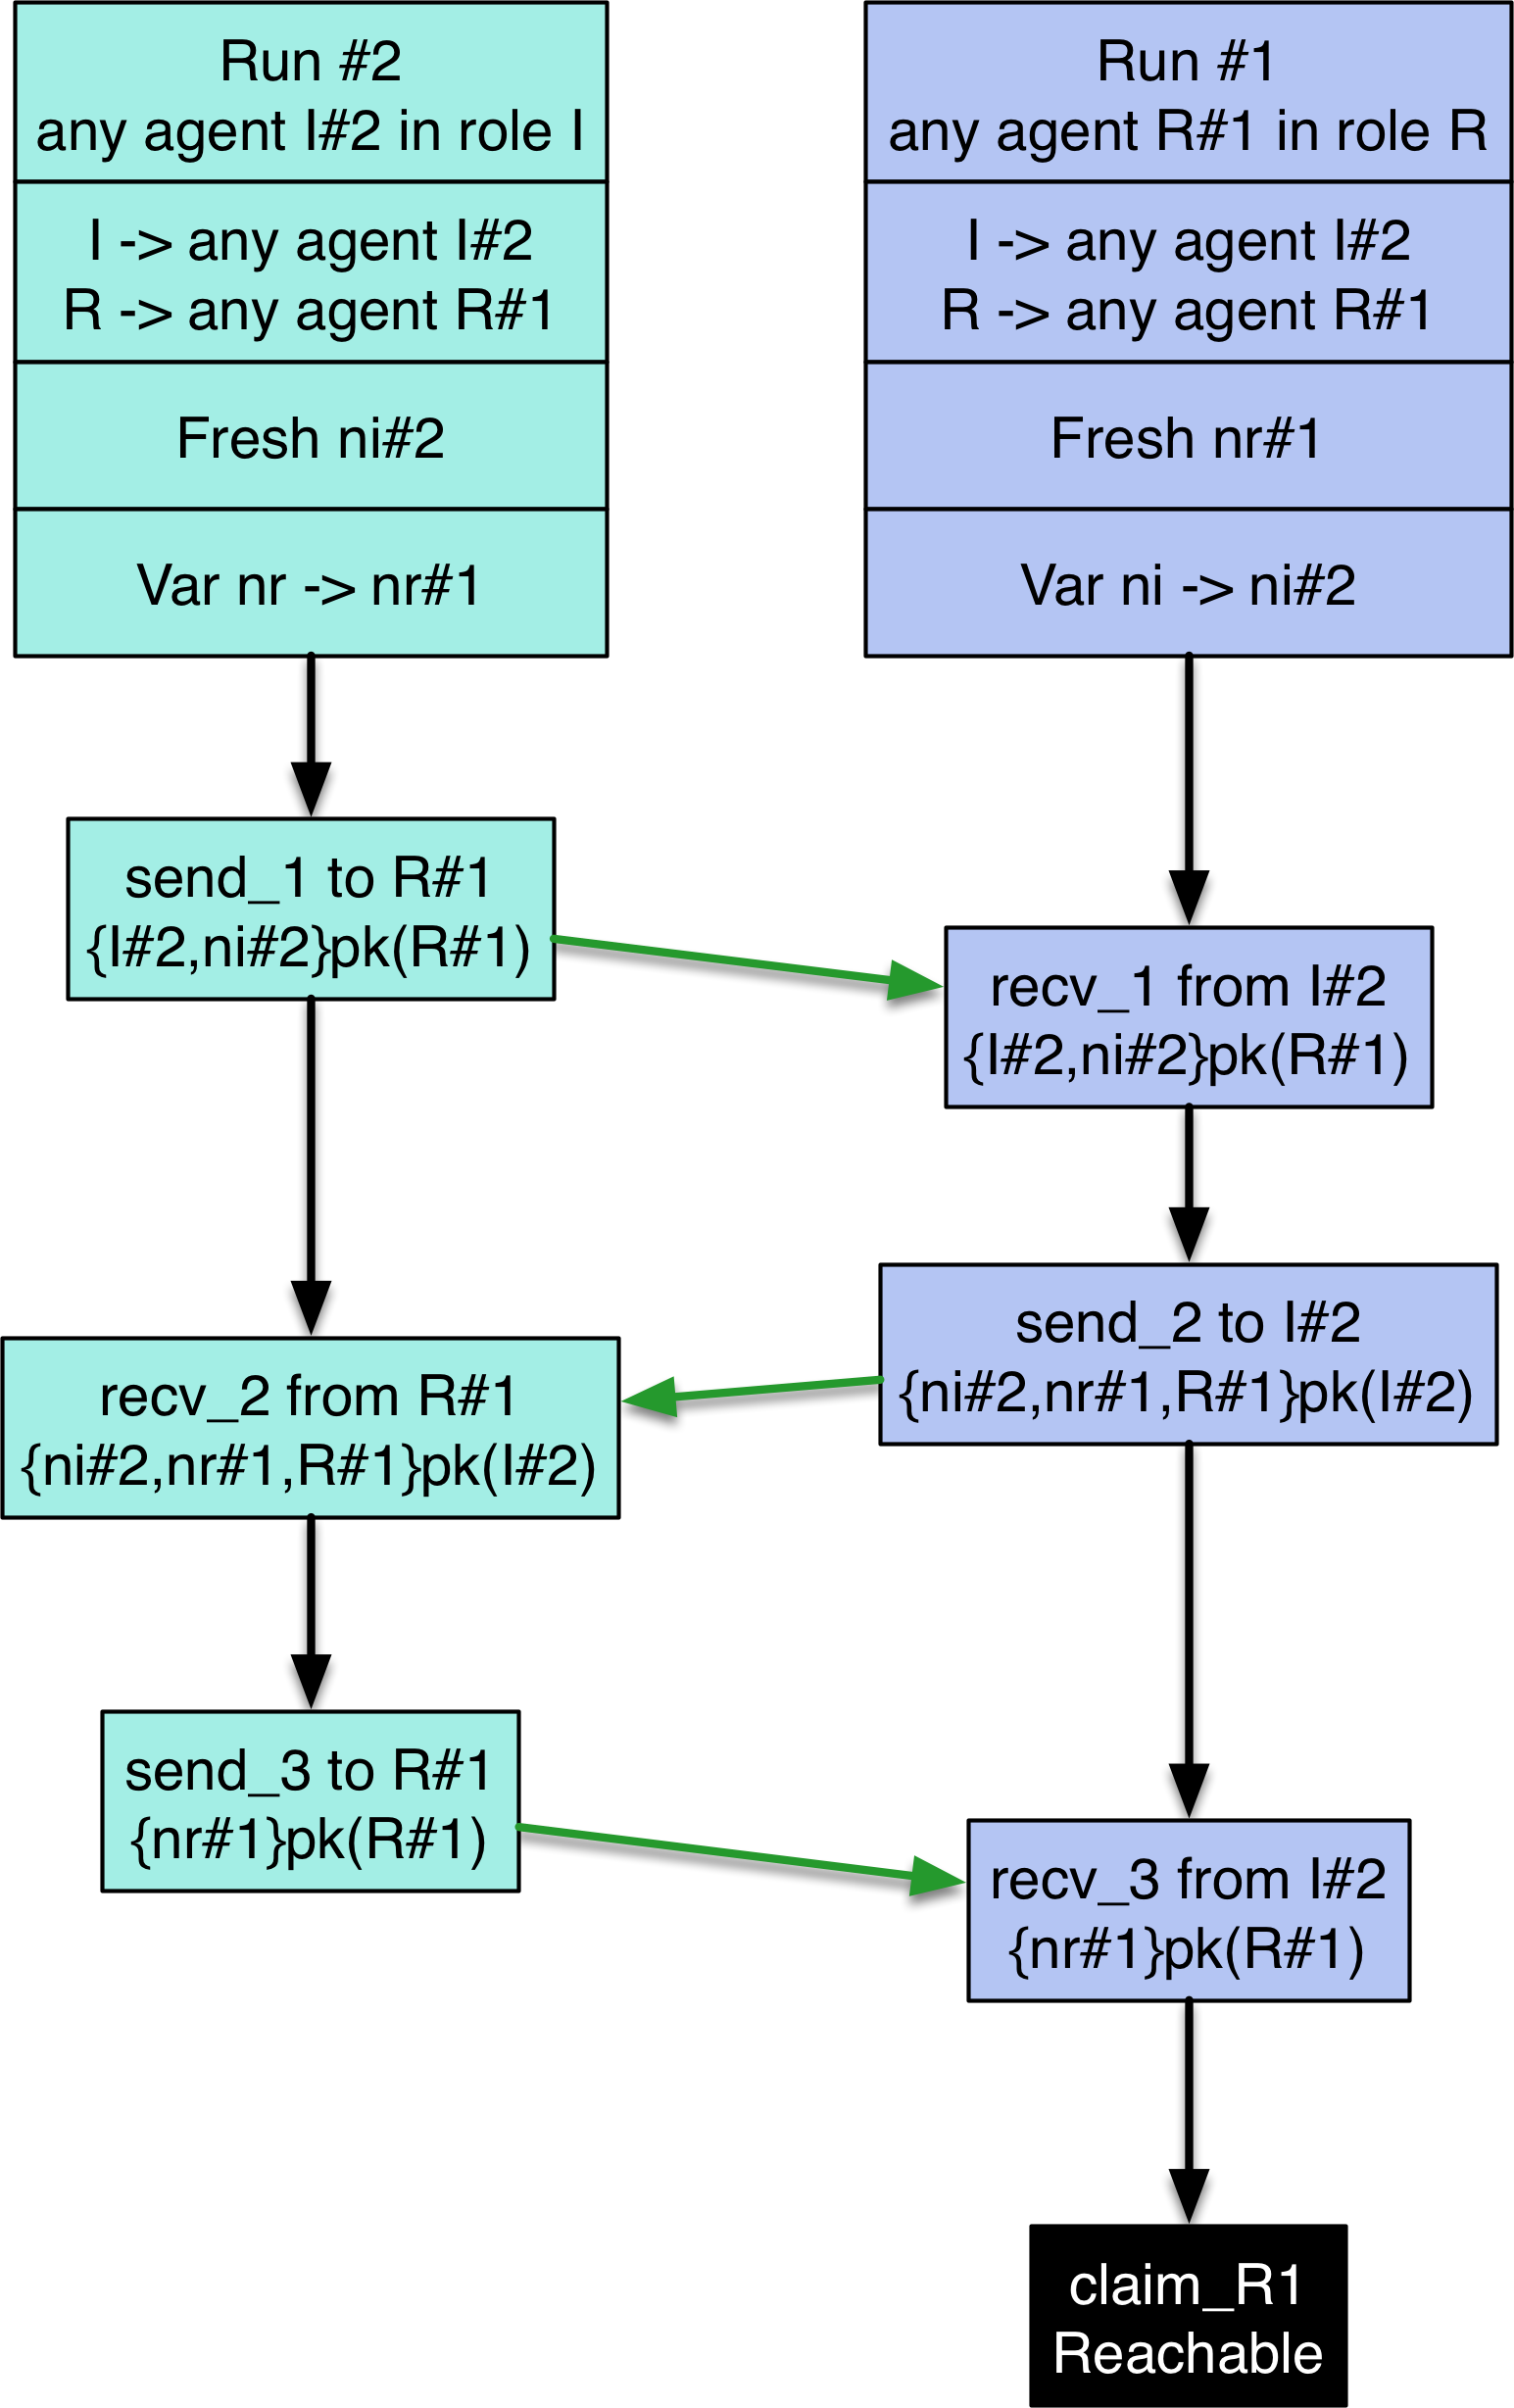
\includegraphics[width=0.95\textwidth]{unt2.png}
    \vspace{9pt}
    \caption{Dijagram toka za protokol NSL}
    \label{fig:char_nsl}
\end{centering}
\end{subfigure}
\caption{SPDL model i dijagram toka za protokol Needham-Schroeder-Lowe}
\end{figure}

\begin{figure}[htb]
\begin{framed}
\begin{small}
\begin{verbatim}
$ scyther-linux -c nsl.spdl 
claim   nsl,I   Reachable_I1    -       Ok      [exactly 1 variant]
claim   nsl,R   Reachable_R1    -       Ok      [exactly 1 variant]
$ scyther-linux nsl.spdl 
claim   nsl,I   Secret_i1       ni      Ok      [proof of correctness]
claim   nsl,I   Secret_i2       nr      Ok      [proof of correctness]
claim   nsl,I   Niagree_i3      -       Ok      [proof of correctness]
claim   nsl,I   Nisynch_i4      -       Ok      [proof of correctness]
claim   nsl,R   Secret_r1       ni      Ok      [proof of correctness]
claim   nsl,R   Secret_r2       nr      Ok      [proof of correctness]
claim   nsl,R   Niagree_r3      -       Ok      [proof of correctness]
claim   nsl,R   Nisynch_r4      -       Ok      [proof of correctness]
\end{verbatim}
\end{small}
\vspace{-15pt}
\end{framed}
\caption{Rezultati provjere i verifikacije modela protokola NSL}
\label{fig:nsl_char}
\end{figure}

\begin{figure}[H]
\end{figure}


\section{Model predloženog protokola ACAP}

Opis protokola ACAP korištenjem SPDL-a sastoji se od glavnog protokola
(\texttt{protocol acap\{I, R\}}) i pomoćnog protokola (\texttt{protocol
@executability \{DH, O\}}), koji se koristi za operacije vezane uz
Diffie-Hellman razmjenu ključeva.

Glavni protokol ACAP sastoji se od dvije glavne uloge \texttt{I} i \texttt{R}
isto kao i protokol Needham-Schreoder-Lowe. U sklopu uloga definiraju se
varijable koje su specifične za protokol ACAP.

Svakoj ulozi potreban je sljedeći niz varijabli:
\begin{itemize}
    \item eksponent za Diffie-Hellman dogovor ključeva,
    \item nasumične vrijednosti za jednokratno korištenje (engl. \emph{nonce})
	za obje strane,
    \item univerzalna varijabla za zaprimanje javnog dijela Diffie-Hellman
	razmjene,
    \item dvije varijable koje sadrže popise algoritama.
\end{itemize}
Deklaracije varijabli za obje uloge prikazane su na slici \ref{fig:var_def}. 

\begin{figure}[htb]
\begin{small}
\begin{verbatim}
protocol acap(I,R) {
  role I {
    # stvaranje novog DH eksponenta i noncea
    fresh i, Ni: Nonce;
    # varijabla za zaprimanje noncea
    var Nr: Nonce;
    # varijabla za zaprimanje javnog dijela DH razmjene
    var Gr: Ticket;
    # stvaranje novog popisa algoritama
    fresh Li: AlgList;
    # varijabla za zaprimanje popisa algoritama
    var Lr: AlgList;
    ...
  }
  role R {
    fresh r, Nr: Nonce; var Ni: Nonce;
    var Gi: Ticket;
    fresh Lr: AlgList; var Li: AlgList;
    ...
  }
}
\end{verbatim}
\end{small}
\vspace{-15pt}
\caption{Prikaz varijabli za uloge započinjatelja i primatelja}
\label{fig:var_def}
\end{figure}

Nakon definicije varijabli i njihovog stvaranja slijedi tijek razmjene poruka
između komunicirajućih strana. Da bi dvije uloge unutar protokola uspješno
razmijenile poruke nužno je da svaki događaj slanja poruke ima odgovarajući
događaj primanja poruke s druge strane. Na slici \ref{fig:i_msgs} prikazani su
događaji slanja i primanja na strani započinjatelja dok je na slici
\ref{fig:r_msgs} prikazano isto za ulogu primatelja.

\begin{figure}[htb]
\begin{small}
\begin{verbatim}
  role I {
    ...
    send_1( I, R, g(i), Ni);
    recv_!2( R, I, Gr, Nr, R, {h(Gr)}sk(R), MAC(h(Gr,i), R, Ni, Nr) );
    send_!3( I, R, I, Li, {h(Li, g(i), Gr)}sk(I), MAC(h(Gr,i), I) );
    recv_4( R, I, Lr, {h(g(i), Gr, Lr)}sk(R) );
    ...
  }
\end{verbatim}
\end{small}
\vspace{-15pt}
\caption{Komunikacija sa strane započinjatelja}
\label{fig:i_msgs}
\end{figure}

\begin{figure}[htb]
\begin{small}
\begin{verbatim}
  role R {
    ...
    recv_1( I, R, Gi, Ni);
    send_!2( R, I, g(r), Nr, R, {h(g(r))}sk(R), MAC(h(Gi,r), R, Ni, Nr) );
    recv_!3( I, R, I, Li, {h(Li, Gi, g(r))}sk(I), MAC(h(Gi,r), I) );
    send_4( R, I, Lr, {h(Gi, g(r), Lr)}sk(R) );
    ...
  }
\end{verbatim}
\end{small}
\vspace{-15pt}
\caption{Komunikacija sa strane primatelja}
\label{fig:r_msgs}
\end{figure}

Prvi događaj slanja (\texttt{send\_1( I, R, g(i), Ni);}) ide od uloge \texttt{I}
prema ulozi \texttt{R} i sadrži parametre definirane za poruku \initi{}.
Odgovarajući događaj
primanja (\texttt{recv\_1( I, R, Gi, Ni);}) definira da poruka dolazi od uloge
\texttt{I}, a prima ju uloga \texttt{R}. Ovakav način pozivanja označava
komunikaciju između uloga \texttt{I} i \texttt{R}.
    
U danom je primjeru vidljivo da događaj \texttt{send\_1} odgovara događaju
\texttt{recv\_1} uz jednakost izraza \texttt{g(i)} i \texttt{Gi}. Isto vrijedi i
za izraze \texttt{send\_4} i \texttt{recv\_4} ako se u obzir uzme i jednakost
\texttt{g(r)} i \texttt{Gr}. Navedene jednakosti su potrebne kako bi
komunicirajuće strane mogle izvesti potrebne operacije.

U modelu je potrebno specificirati i zasebnu ulogu koja će omogućiti razmjenu
poruka definiranu događajima \texttt{send\_!2} i \texttt{recv\_!2} te
\texttt{send\_!3} i \texttt{recv\_!3} koji izravno ne odgovaraju jedan drugome.
Ti događaji uključuju poseban znak \texttt{!} (uskličnik), koji specificira da se
poruka šalje svim ulogama koje su dostupne u sklopu procesa verifikacije, a ne
samo između definiranih primatelja i pošiljatelja. Uloge u procesu verifikacije
obuhvaćaju sve definirane uloge, uključujući i ulogu napadača.
U sljedećem potpoglavlju dan je opis dodatnog protokola za modeliranje
Diffie-Hellman operacija.

\subsection{Modeliranje Diffie-Hellman operacija}

U alatu Scyther v1.1.3, koja je bila dostupna za vrijeme pisanja
disertacije nije podržano izravno korištenje Diffie-Hellman operacija.
Stoga je potrebno napraviti apstrakciju s pomoću integriranih operacija.
Diffie-Hellman (DH) operacije izračunavanja zamijenjene su jednosmjernom
funkcijom. DH operacija definirana izrazom $A = g^a mod p$ zamijenjena je
funkcijom g (\texttt{hashfunction g}) i izrazom \texttt{g(a)}, zbog pretpostavke
da operacija nije
reverzibilna, što vrijedi za tu vrstu potenciranja i računanja ostatka kao i za
funkciju sažetka unutar alata Scyther. Zbog tog svojstva primatelj podataka
poslanu informaciju \texttt{g(i)} prima pomoću univerzalne varijable
\texttt{Ticket Gi}.

Drugi dio DH izračuna odrađuje se s pomoću funkcije sažetka h
(\texttt{hashfunction h}) i rezultat te operacije je zajednička tajna u sklopu
DH razmjene. Izraz $S = (g^a mod p)^b$ istovjetan je izrazu \texttt{h(g(a),b)}.
Potrebno je i definirati da je operacija komutativna kako bi eventualni napadač uz
poznavanje jednog tajnog dijela DH razmjene (\texttt{a} ili \texttt{b}) mogao
doći do razmijenjene tajne. To je izvedeno s pomoću uloge \texttt{DH} u pomoćnom
protokolu (\texttt{@executability}) kojim se postiže jednakost \texttt{h(g(r),i)
= h(g(i),r)}, kako je prikazano na slici \ref{fig:exec_dh}. U toj specifikaciji je
korišten simbol uskličnika kod slanja i primanja kako bi ta jednakost vrijedila
za sve definirane uloge i napadača.

\begin{figure}[htb]
\begin{small}
\begin{verbatim}
protocol @executability (DH, O) {
  role DH {
    # definicija DH eksponenata
    var i, r: Nonce;
    # primi od bilo kojeg pošiljatelja
    recv_!DH1( DH, DH, h(g(r),i) );
    # pošalji bilo kojem primatelju ekvivalentni izraz
    send_!DH2( DH, DH, h(g(i),r) );
  }
  role O { ... }
}
\end{verbatim}
\end{small}
\vspace{-22pt}
\caption{Komutativnost Diffie-Hellman operacije}
\label{fig:exec_dh}
\end{figure}

Pomoćni protokol sadrži još jednu ulogu \texttt{O} koja se koristi za uspješnu
razmjenu poruka \initr{} i \listi{}, koje koriste zajedničku tajnu uspostavljenu
kroz DH za stvaranje zaštitnog HMAC sažetka. Uloga \texttt{O}
prikazana je na slici \ref{fig:exec_o}. Razmjena poruka između uloga \texttt{I}
i \texttt{R} odvija se kroz tu ulogu. Na slici su prikazani događaji
\texttt{send} i \texttt{recv} koji su povezani tom ulogom.

\begin{figure}[H]
\begin{small}
\begin{verbatim}
role O {
  var i, r, Ni, Nr: Nonce;
  var I, R: Agent; var Li: AlgList;
  ### razmjena poruke INITr (R->I) ###
  #send događaj u ulozi R
  #send_!2( R, I, g(r), Nr, R, {h(g(r))}sk(R), MAC(h(  Gi,r), R, Ni, Nr) );
  recv_!01( O, O, g(r), Nr, R, {h(g(r))}sk(R), MAC(h(g(i),r), R, Ni, Nr) );
  send_!02( O, O, g(r), Nr, R, {h(g(r))}sk(R), MAC(h(g(r),i), R, Ni, Nr) );
  #recv događaj u ulozi I
  #recv_!2( R, I,   Gr, Nr, R, {h(  Gr)}sk(R), MAC(h(  Gr,i), R, Ni, Nr) );
  ### razmjena poruke LISTi (I->R) ###
  #send događaj u ulozi I
  #send_!3( I, R, I, Li, {h(Li, g(i),   Gr)}sk(I), MAC(h(  Gr,i), I) );
  recv_!03( O, O, I, Li, {h(Li, g(i), g(r))}sk(I), MAC(h(g(r),i), I) );
  send_!04( O, O, I, Li, {h(Li, g(i), g(r))}sk(I), MAC(h(g(i),r), I) );
  #recv događaj u ulozi I
  #recv_!3( I, R, I, Li, {h(Li,   Gi, g(r))}sk(I), MAC(h(  Gi,r), I) );
}
\end{verbatim}
\end{small}
\vspace{-22pt}
\caption{Razmjena poruka \initr{} i \listi{} definirana u ulozi \texttt{O}}
\label{fig:exec_o}
\end{figure}

\section{Formalna verifikacija modela}
\label{sec:verif}
Prvi korak provjere ispravnosti modela je provjera
uspješnog završetka komunikacije s obje strane.
Alat Scyther nakon uspješne provjere generira dijagram toka za
specificirani model. Dijagram toka za model protokola ACAP prikazan je na slici
\ref{fig:characterize}. 

\begin{figure}[H]
\begin{centering}
    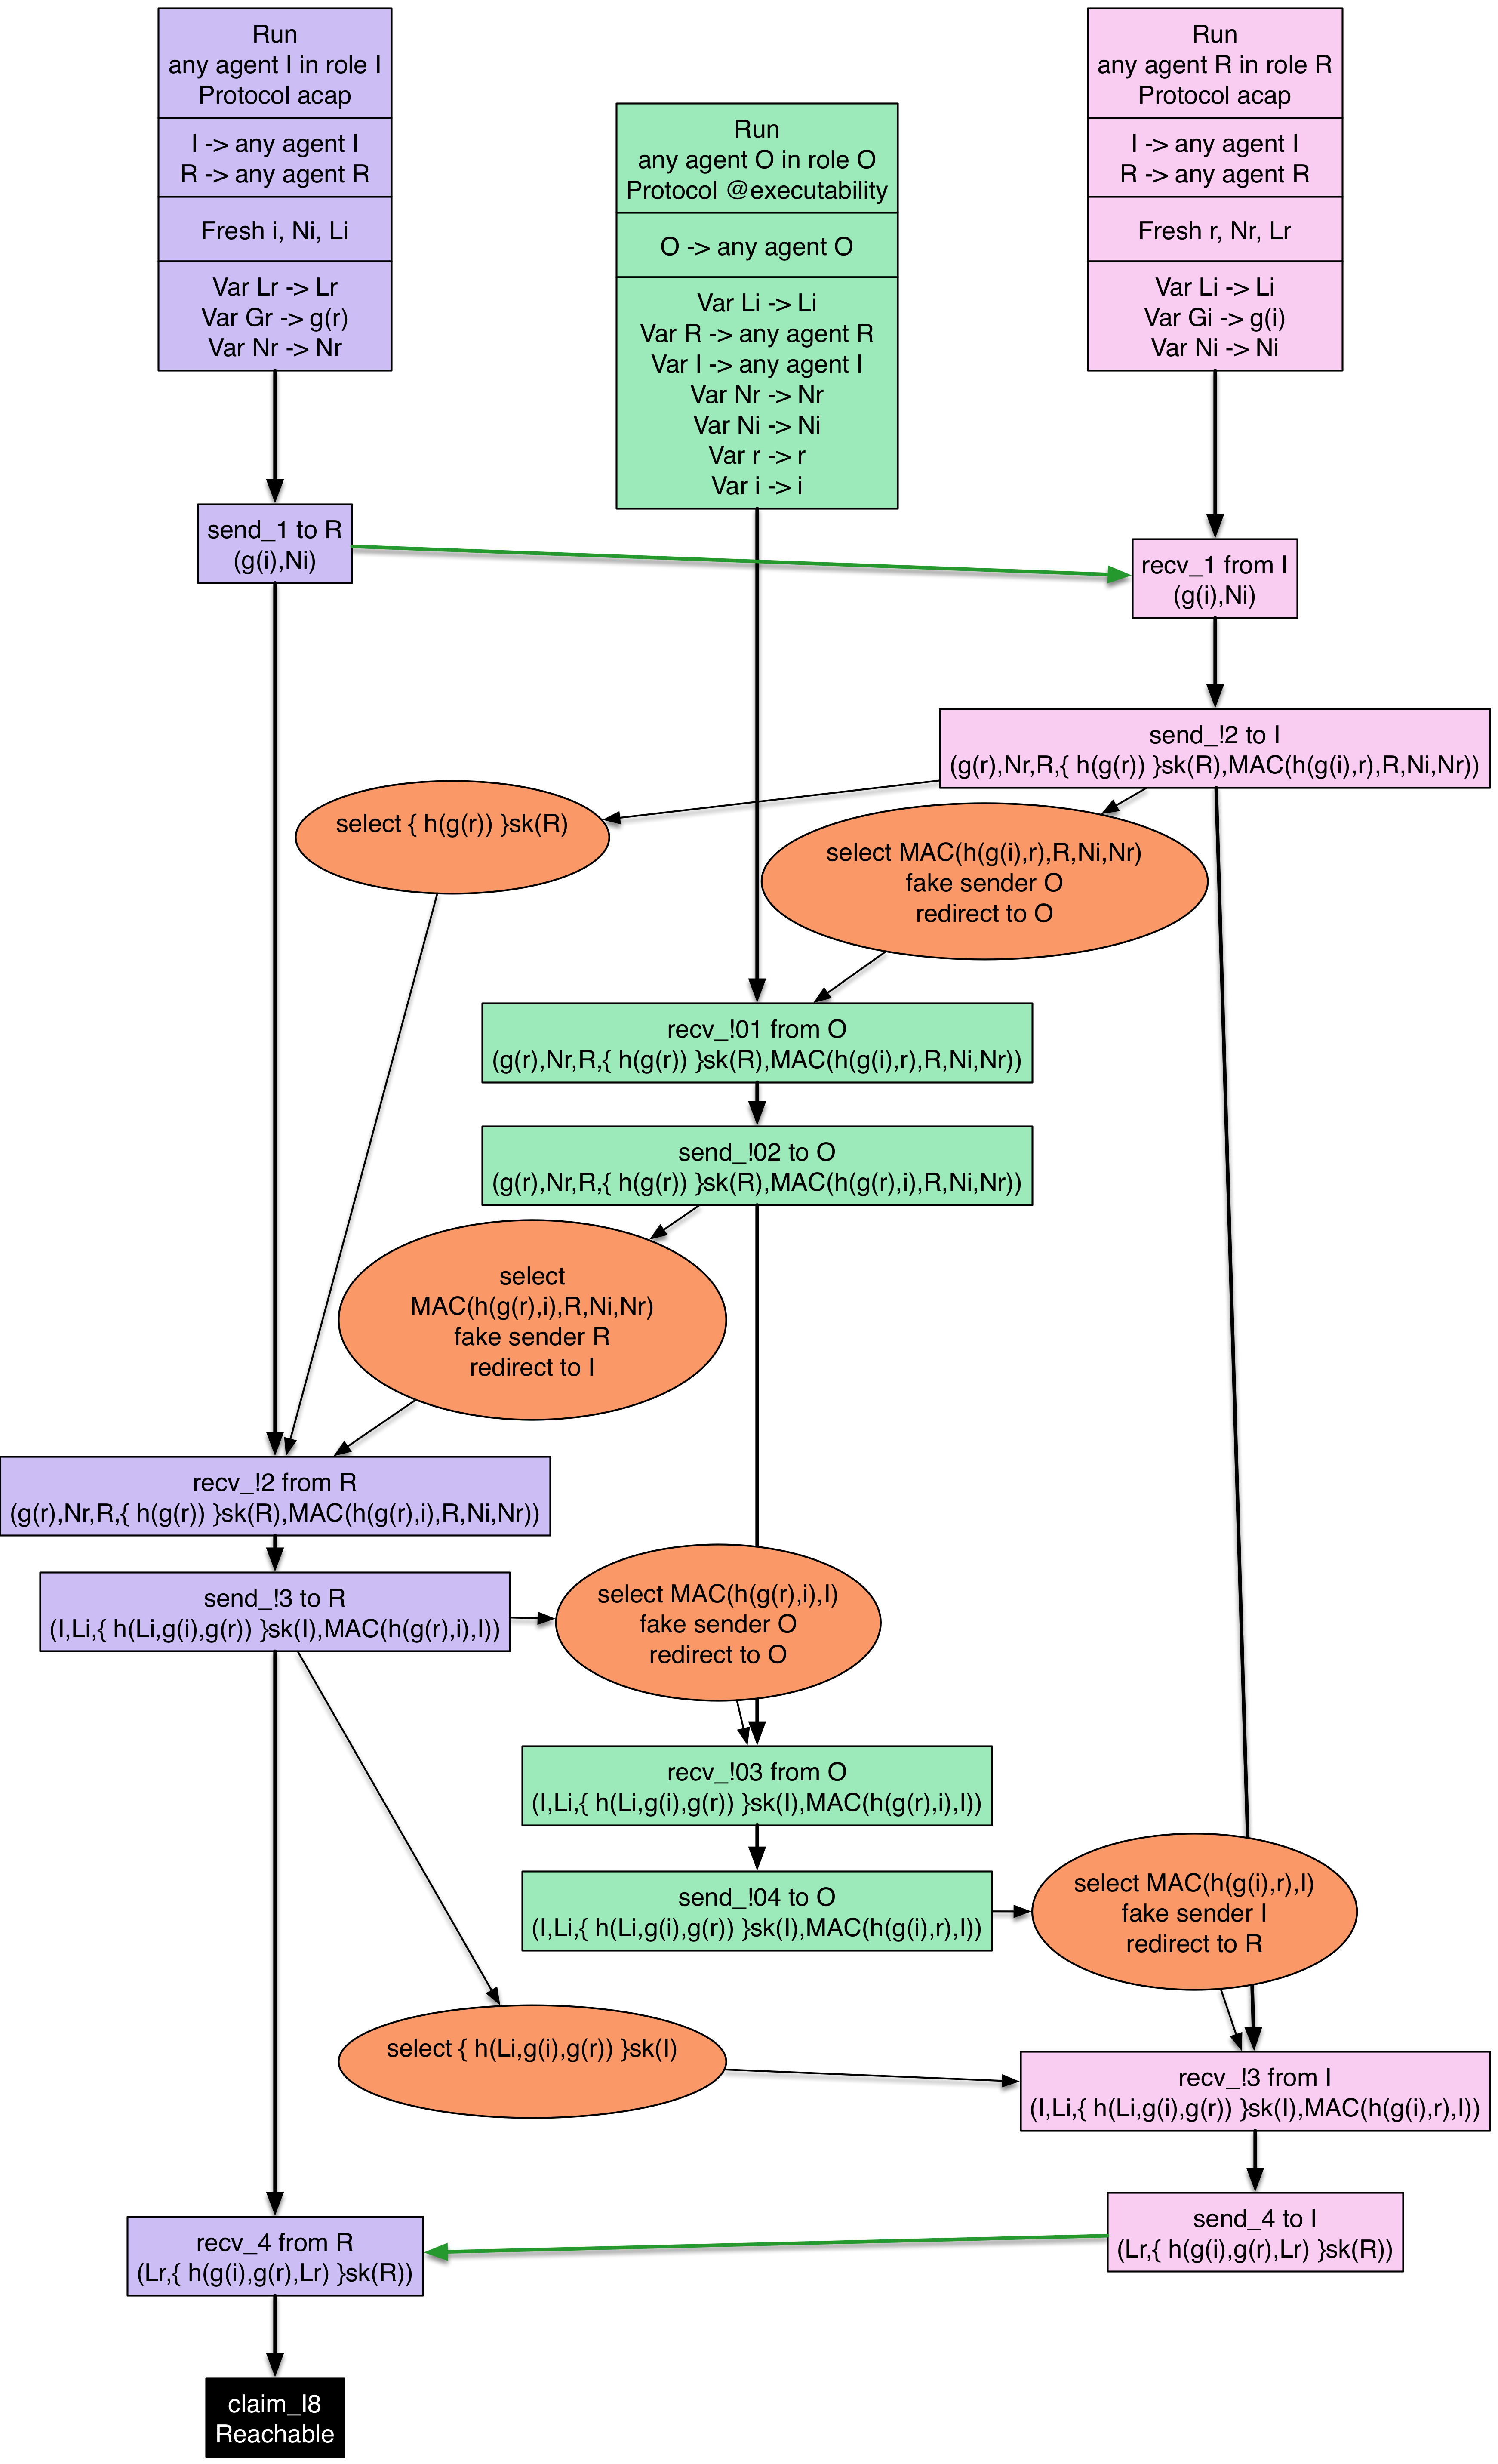
\includegraphics[width=0.75\textwidth]{graf}
    \caption{Dijagram toka za protokol ACAP}
    \label{fig:characterize}
\end{centering}
\end{figure}

Na slici se vidi da su za jednu uspješnu razmjenu
poruka potrebne tri uloge: uloga započinjatelja (\texttt{Role I}) i uloga
primatelja (\texttt{Role R}) u sklopu glavnog protokola i dodatna uloga za
upravljanje DH razmjenom (\texttt{Role O}) u sklopu pomoćnog protokola.

\subsection{Definicija sigurnosnih zahtjeva}

Nakon definiranja poruka i tijeka komunikacije, za svaku ulogu u modelu potrebno
je
odrediti sigurnosne zahtjeve koji trebaju biti zadovoljeni. Sigurnosni zahtjevi
za modelirani protokol su sljedeći:
\begin{itemize}
    \item Javni dijelovi DH razmjene moraju ostati nepromijenjeni za vrijeme
	razmjene kako bi obje strane imale istu zajedničku tajnu za vrijeme
	komunikacije. To se provjerava s pomoću sigurnosnog zahtjeva
	\texttt{claim} s ključnim riječima \texttt{Running} i \texttt{Commit}.
    \item Zajednička tajna ni u jednom trenutku tijekom razmjene ne smije doći do
	uloge napadača. Ta tvrdnja se provjerava koristeći ključnu riječ
	\texttt{SKR} (engl. \emph{Session Key Reveal}) koja označava otkrivanje ključa
	trenutne sjednice.
    \item Napadač ne smije imati nikakav utjecaj na razmjenu poruka, što
	predstavlja otpornost protokola na napade ponavljanja i napade s
	napadačem u sredini (\emph{man in the middle}). Sigurnosni zahtjev
	postavlja se s ključnom riječi \texttt{Nisynch} koja predstavlja pojam ne
	injektivne sinkronizacije (engl. \emph{Non-injective synchronization})
	\cite{scyther_book}.
\end{itemize}

Definirani sigurnosni zahtjevi prikazani su na slici \ref{fig:claims}.

\begin{figure}[htb]
\begin{small}
\begin{verbatim}
role R {
  recv_1( I, R, Gi, Ni);
  # početak praćenja javnih dijelova DH razmjene
  claim_R1( R, Running, I, g(r), Gi);
  send_!2( ... ); recv_!3( ... ); send_4( ... );

  # provjera istovjetnosti početnih i krajnjih vrijednosti
  claim_R2( R, Commit, I, g(r), Gi);
  # zahtjev tajnosti nad zajedničkom tajnom
  claim_R3( R, SKR, KDF(h(Gi,r)) );
  # zahtjev da napadač nije u mogućnosti utjecati na komunikaciju
  claim_R4( R, Nisynch );
}
\end{verbatim}
\end{small}
\vspace{-15pt}
\caption{Definicija sigurnosnih zahtjeva za modelirani protokol}
\label{fig:claims}
\end{figure}
\vspace{-10pt}

\subsection{Rezultati formalne verifikacije}

Verificirani model protokola ACAP nalazi se u dodatku \ref{app:model}.
Na adresi \url{http://public.tel.fer.hr/acap} nalazi se potpuni model i
rezultati verifikacije uz programsko ostvarenje i primjer izvođenja.
Prilikom pokretanja
verifikacije moguće je odrediti broj paralelnih uloga koje će se izvoditi u
pokušaju napada na protokol. Moguće je verificirati i uz neograničen broj
paralelnih uloga, što u potpunosti dokazuje istinitost definiranih sigurnosnih
zahtjeva. Model protokola ACAP verificiran je uz neograničen broj paralelnih
uloga kod testiranja i pokazano je da su svi definirani sigurnosni zahtjevi
zadovoljeni.  
Rezultati verifikacije s alatom Scyther prikazani su na slici
\ref{fig:verif_res}.
Zahtjevi \texttt{I2} i \texttt{R2} pokazuju da ne dolazi do promjene parametara
DH razmjene,
zahtjevi \texttt{I3} i \texttt{R3} pokazuju da zajednička tajna nije otkrivena,
a zahtjevi \texttt{I4} i \texttt{R4} da napadač ne može utjecati na razmjenu
poruka.

\begin{figure}[ht]
\begin{centering}
\begin{framed}
\begin{small}
\begin{verbatim}
$ scyther-linux acap.spdl
claim   acap,I  Commit_I2       (R,g(i),Gr)     Ok  [no attack within bounds]
claim   acap,I  SKR_I3  KDF(h(Gr,i))    Ok      [no attack within bounds]
claim   acap,I  Nisynch_I4      -       Ok      [no attack within bounds]
claim   acap,R  Commit_R2       (I,g(r),Gi)     Ok  [no attack within bounds]
claim   acap,R  SKR_R3  KDF(h(Gi,r))    Ok      [no attack within bounds]
claim   acap,R  Nisynch_R4      -       Ok      [no attack within bounds]
\end{verbatim}
\end{small}
\vspace{-15pt}
\end{framed}
\vspace{-15pt}
\caption{Rezultati verifikacije protokola s alatom Scyther}
\label{fig:verif_res}
\end{centering}
\end{figure}
\vspace{-10pt}

Proces formalne verifikacije posebno je zahtjevan zbog zasebnog modeliranja
Diffie-Hellman operacija koje prouzrokuju veći broj stanja za provjeru nego što
je potrebno. Zahtjevnost se očituje u količini vremena i resursa koji su
potrebni za verifikaciju protokola. Što je veći broj paralelnih uloga u
verifikaciji to verifikacija traje dulje i veći su zahtjevi na radnu memoriju
(RAM) u sustavu.
Formalna verifikacija izvodila se na 6 jezgara procesora Intel Xeon E5-2680
(frekvencije 2.70 Ghz) s 40 GB radne memorije. Trajanje verifikacije
prikazano je u tablici \ref{tab:verif_dur}. Verifikacija se izvodila paralelno
na svih 6 jezgara kako bi se skratilo vrijeme izvođenja verifikacije, ali to je
ujedno i povećalo zahtjeve za radnom memorijom.

\begin{table}[htb]
\caption{Trajanje formalne verifikacije ovisno o broju paralelnih uloga}
\renewcommand{\arraystretch}{1.25}
\label{tab:verif_dur}
\centering
\small
\begin{tabular}{ c  c }
\toprule
Broj uloga & Trajanje verifikacije (min)
    \\ \midrule
%    3 & 0.2
%    \\ \hline
    4 & 2.3 
    \\ \hline
    5 & 13.0
    \\ \hline
    6 & 52.0
    \\ \hline
    7 & 174.0
    \\ \hline
    8 & 457.0
    \\ \hline
    9 & 877.0
    \\ \hline
    10 & 1255.0
    \\ \hline
    neograničen & 1532.0
    \\ \bottomrule
\end{tabular}
\end{table}

Prema dobivenim vrijednostima trajanja verifikacije može se zaključiti kako se
povećavanjem broja uloga značajno povećava broj stanja koje je potrebno
provjeriti, što iziskuje veću količinu vremena. Može se primijetiti da su
zadnje dvije verifikacije slične po trajanju, što upućuje da je verifikacija s
10 uloga došla blizu maksimalnog broja stanja kojeg je moguće postići sa
specificiranim modelom protokola.


% vim: spell spelllang=hr

\chapter{Primjena protokola za sigurno dogovaranje u okolini Interneta stvari}
\label{ch:iot}

Okolina Interneta stvari predstavlja mnoštvo uređaja različitih mogućnosti koji
su povezani putem Interneta i služe za pružanje raznih usluga, a temelji se na
vjerodostojnom prikupljanju podataka i pouzdanom upravljanju uređajima unutar
okoline.

Uređaji koji komuniciraju u okolini Interneta stvari često raspolažu ograničenim
mogućnostima. Temeljne mogućnosti uređaja Interneta stvari su:
\begin{itemize}
    \item vrsta i trenutna razina izvora napajanja,
    \item propusnost i kvaliteta mrežne povezanosti i
    \item računalna snaga na raspolaganju.
\end{itemize}

Uređaji u okolini Interneta stvari moraju biti u mogućnosti međusobno sigurno
komunicirati i pružati određenu razinu usluge. To se postiže s pomoću
sigurne komunikacije. Sigurna komunikacija zasniva se na prilagodljivom
dogovoru kriptografskih algoritama i potrebnih ključeva, koji je izveden u
sklopu
predloženog protokola ACAP. Uz protokol se koriste dodatne operacije zaštite
koje koriste rezultate protokola ACAP (dogovorene kriptografske ključeve i
algoritme) kao ulaz za zaštitu podataka ovisno o potrebnoj razini zaštite.

\section{Primjene sigurne komunikacije u okolini Interneta stvari}
\label{sec:scenarios}

Okolina Interneta stvari može se definirati kao slojevita arhitektura koja povezuje
razne uređaje kroz različite mrežne okoline. Cjelokupna arhitektura prikazana je
kroz par ključnih scenarija na slici \ref{fig:iot}, a temelji se na arhitekturi
predstavljenoj u \cite{perera2014context}. Cjelokupna arhitektura sastoji se od
tri osnovna sloja:

\begin{itemize}
\item \textit{Senzorski sloj} predstavlja izvor podataka cijele arhitekture, a
    čine ga uređaji ograničenih računalnih sposobnosti koji prikupljaju podatke
    iz okoline ili obavljaju jednostavne poslove.
\item \textit{Srednji sloj} se koristi za prikupljanje podataka iz senzorskog
    sloja i njihovo prosljeđivanje u gornji sloj računalnog oblaka. Uređaji na
    ovom sloju raspolažu s više resursa i mogu obavljati filtriranje i
    grupiranje podataka srednjeg sloja prije prosljeđivanja.
\item \textit{Sloj računalnog oblaka} predstavlja sloj usluge na kojem se
    obrađuju i skladište podaci koji se prikupljaju u senzorskom sloju, a
    filtriraju u srednjem sloju. Podaci obrađeni na ovom sloju koriste se za
    pronalaženje novih informacija na temelju kojih se upravlja ostatkom
    arhitekture u cilju ostvarivanja kompleksnih usluga upravljanja
    arhitekturom.
\end{itemize}

Osnovne primjene sigurne komunikacije prikazane su na slici \ref{fig:iot}, a
dijele se u četiri osnovne kategorije. Zaštita komunikacije ključna je za
sigurnost cijele platforme kako bi se omogućila provjera autentičnosti
izvora podataka i zaštitila komunikacija između uređaja koja predstavlja temelj
cjelokupne okoline Interneta stvari.

\begin{figure}
    \captionsetup[subfigure]{aboveskip=4pt,belowskip=4pt}
    \centering
    \begin{subfigure}[b]{0.49\textwidth}
        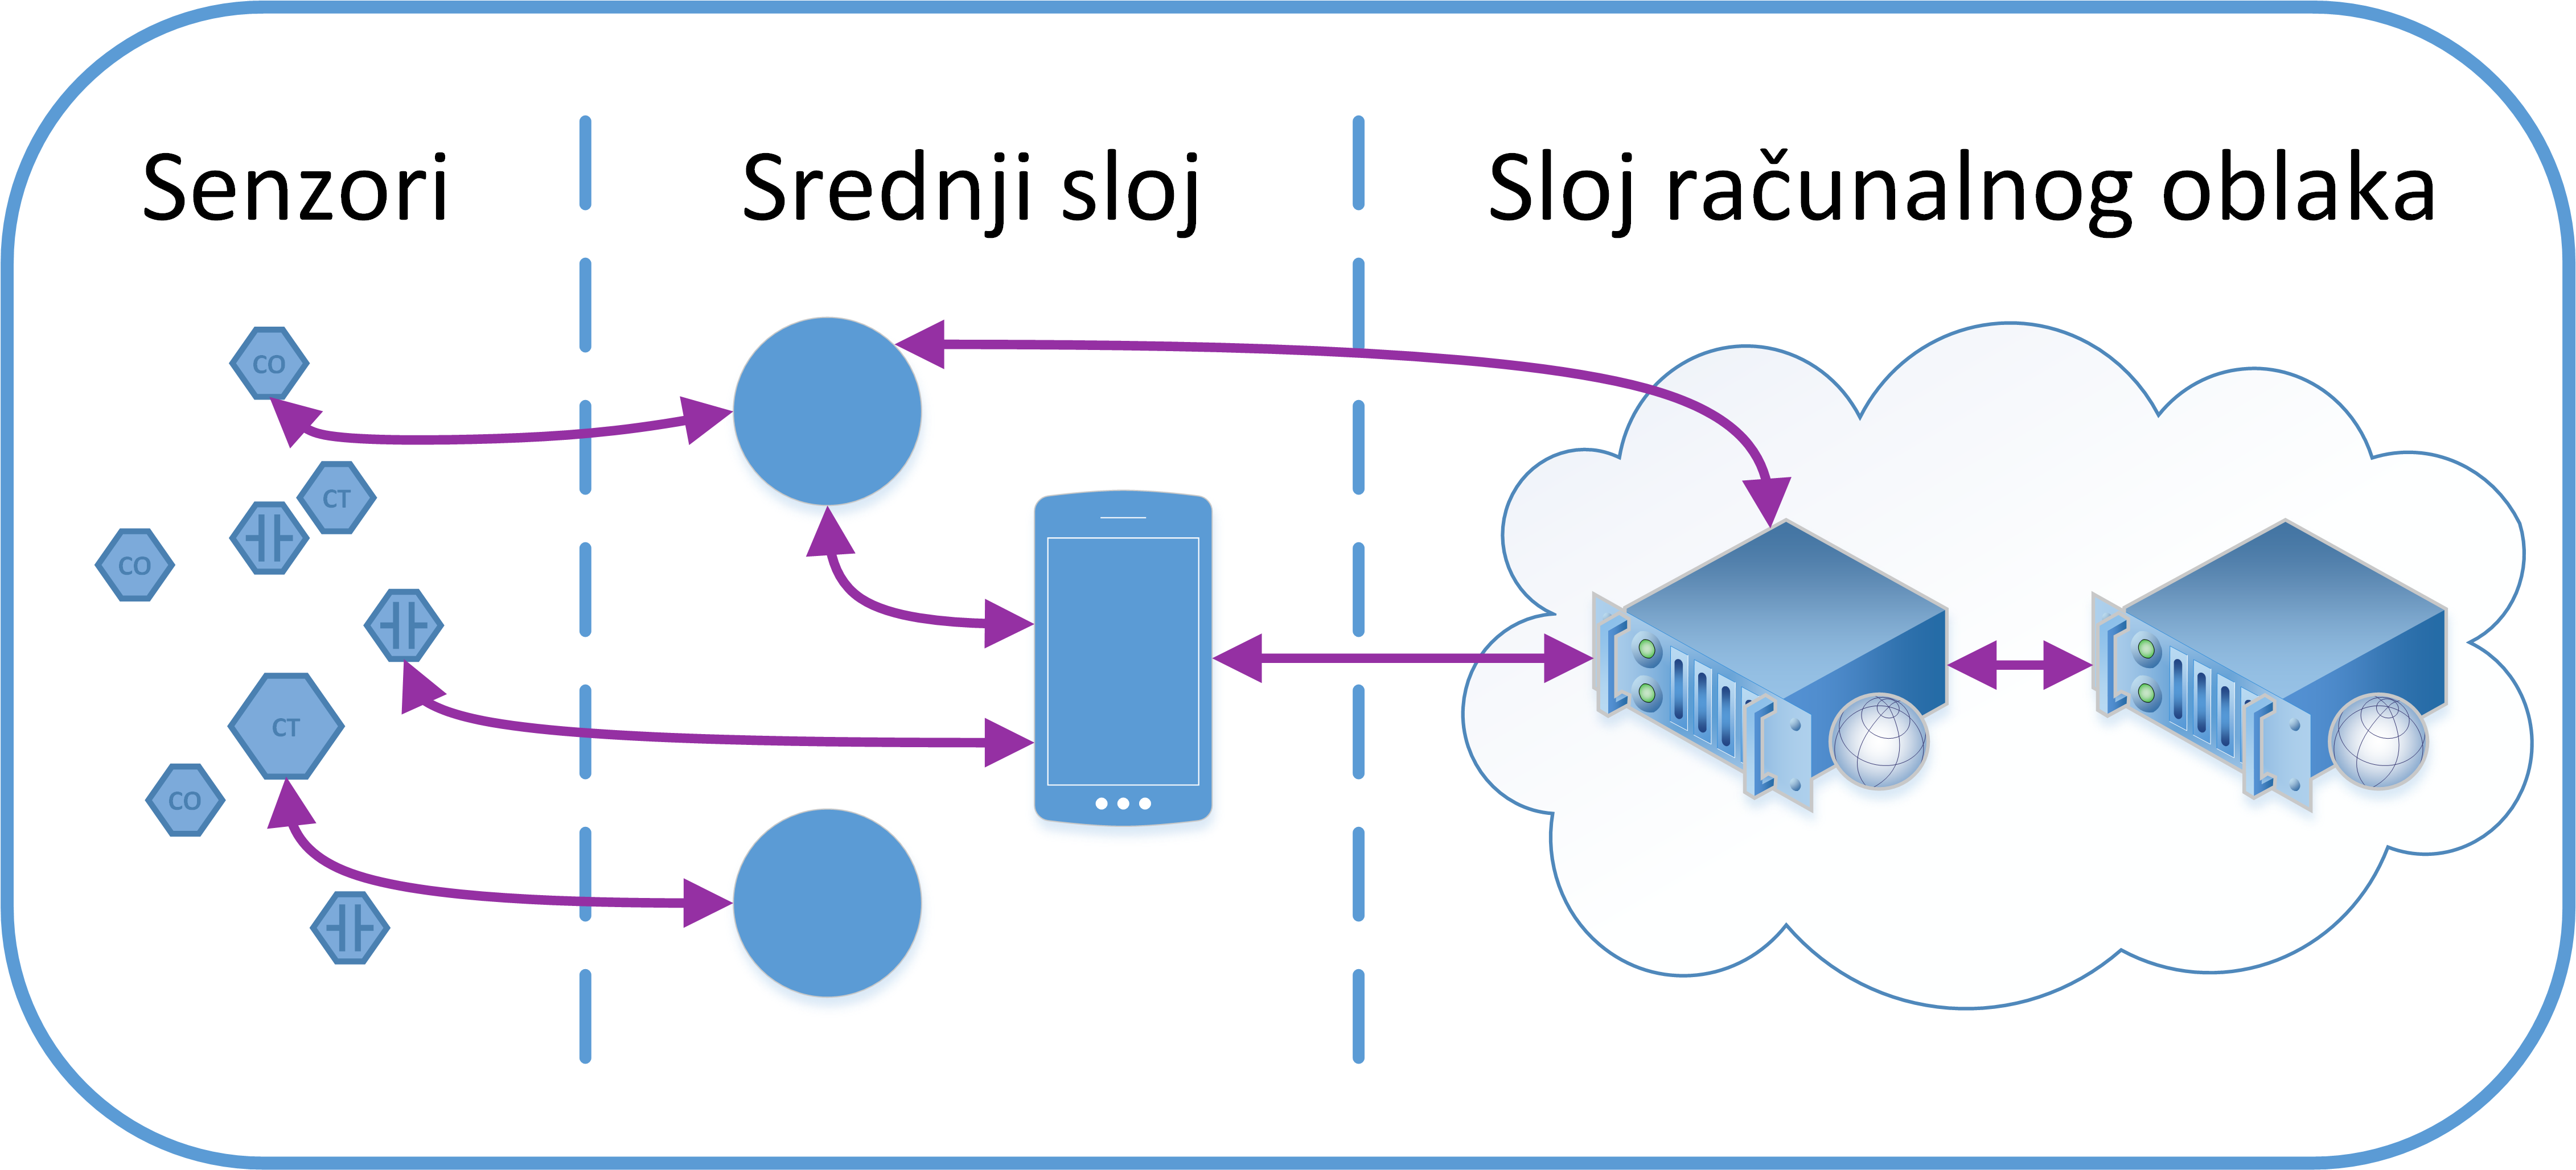
\includegraphics[width=\textwidth]{iot_independent}
        \caption{Arhitektura neovisna o platformi}
	\label{fig:independent}
    \end{subfigure}
    \begin{subfigure}[b]{0.49\textwidth}
        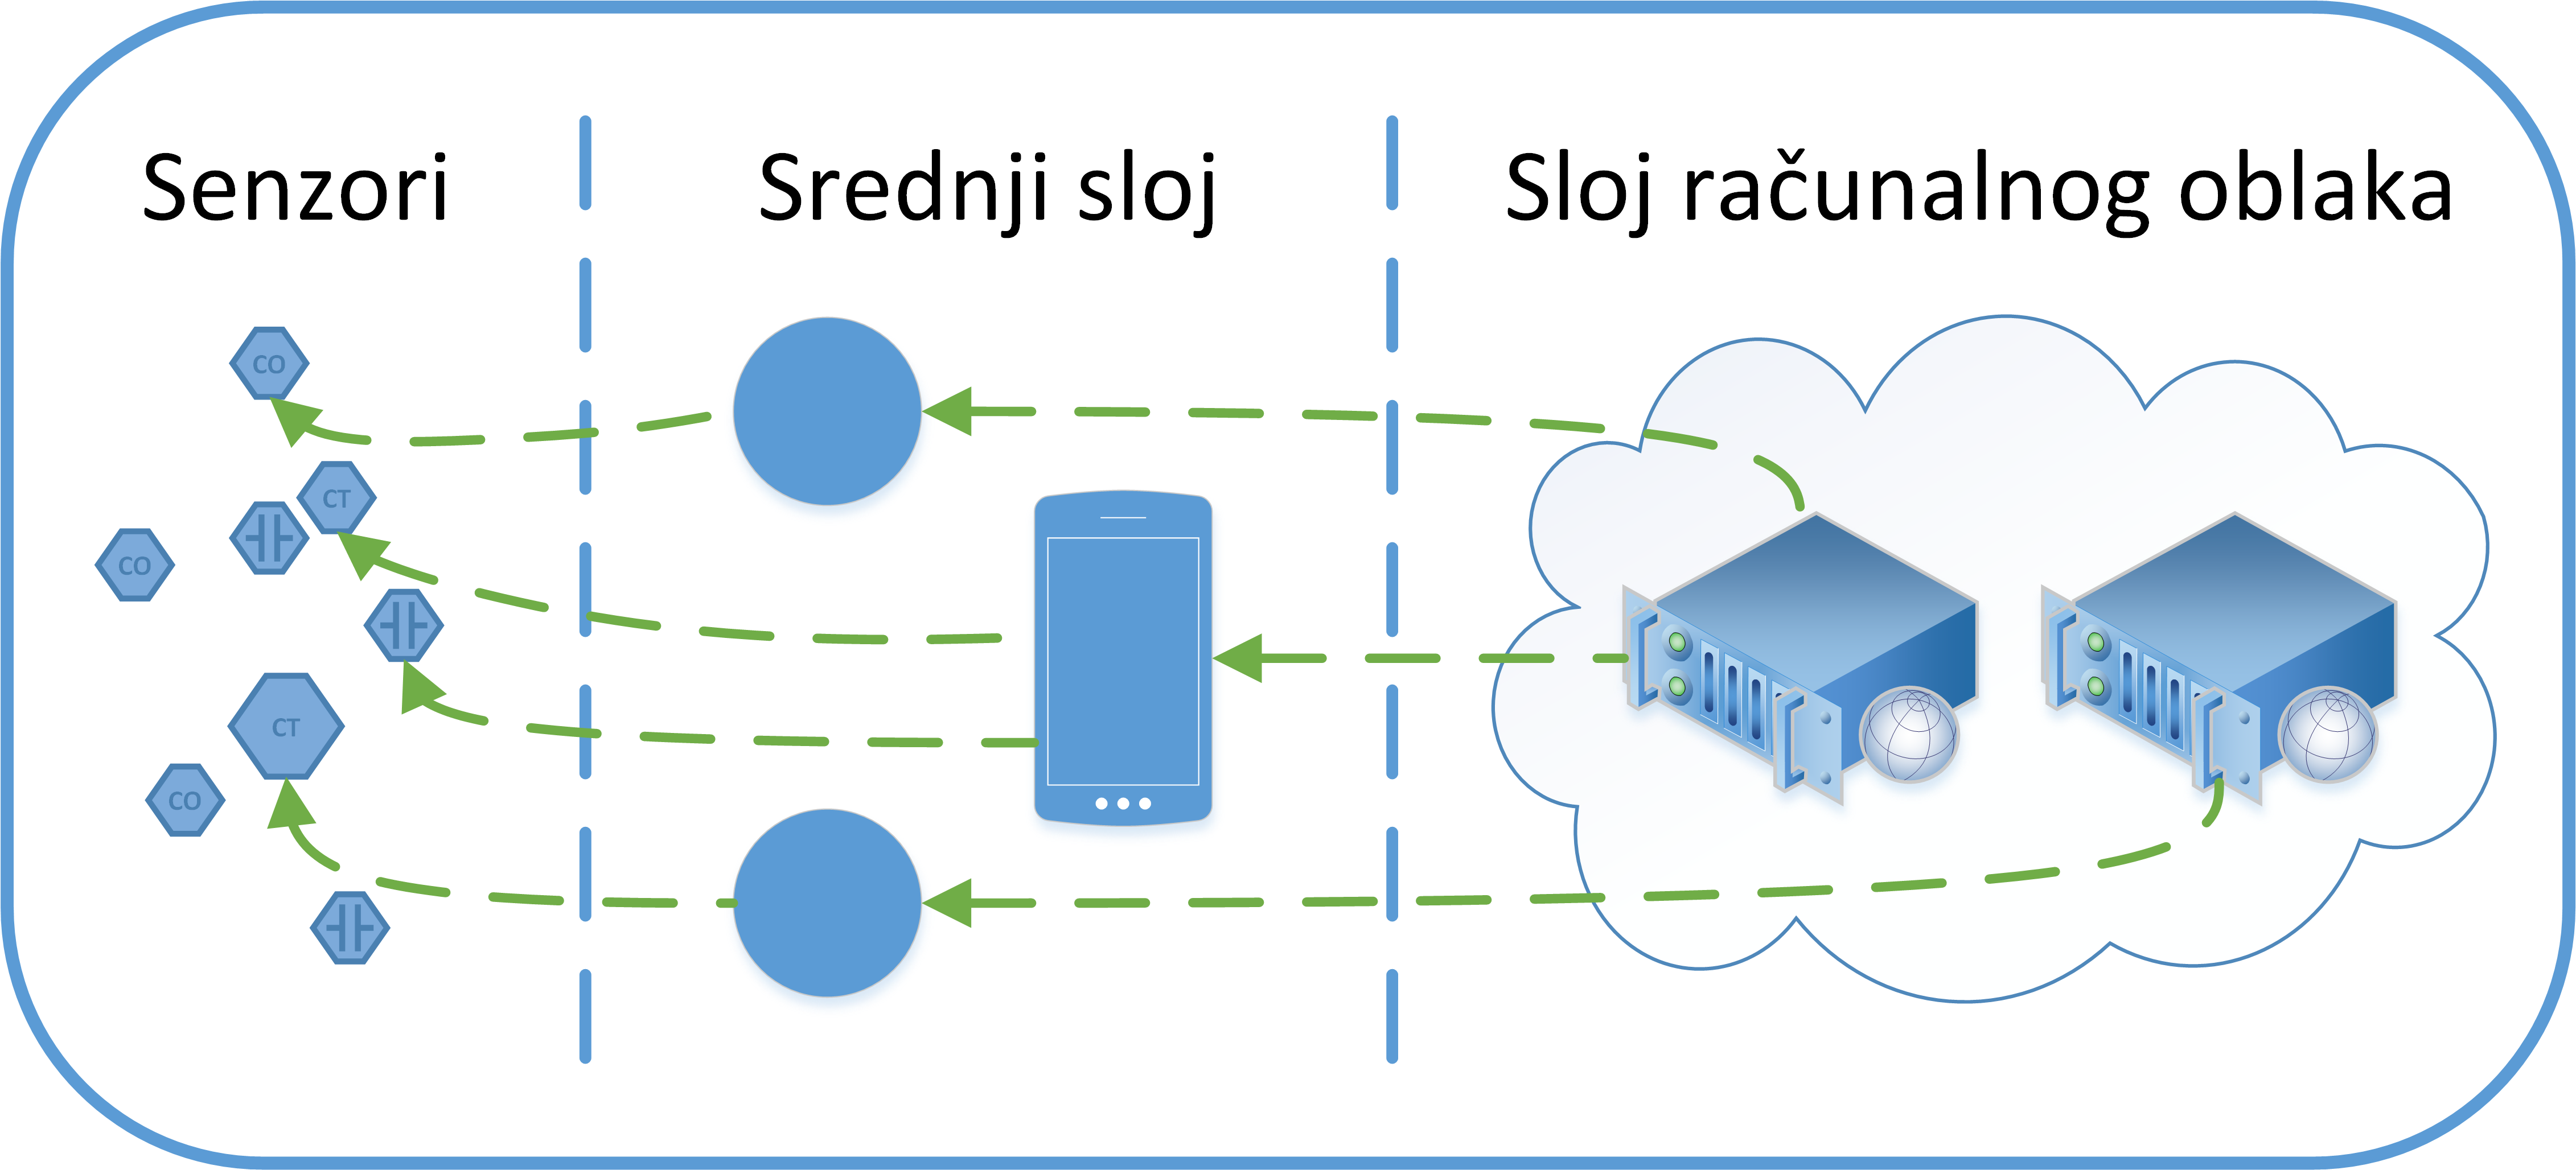
\includegraphics[width=\textwidth]{iot_authenticated}
        \caption{Autentificirano upravljanje uređajima}
	\label{fig:management}
    \end{subfigure}
    \begin{subfigure}[b]{0.49\textwidth}
        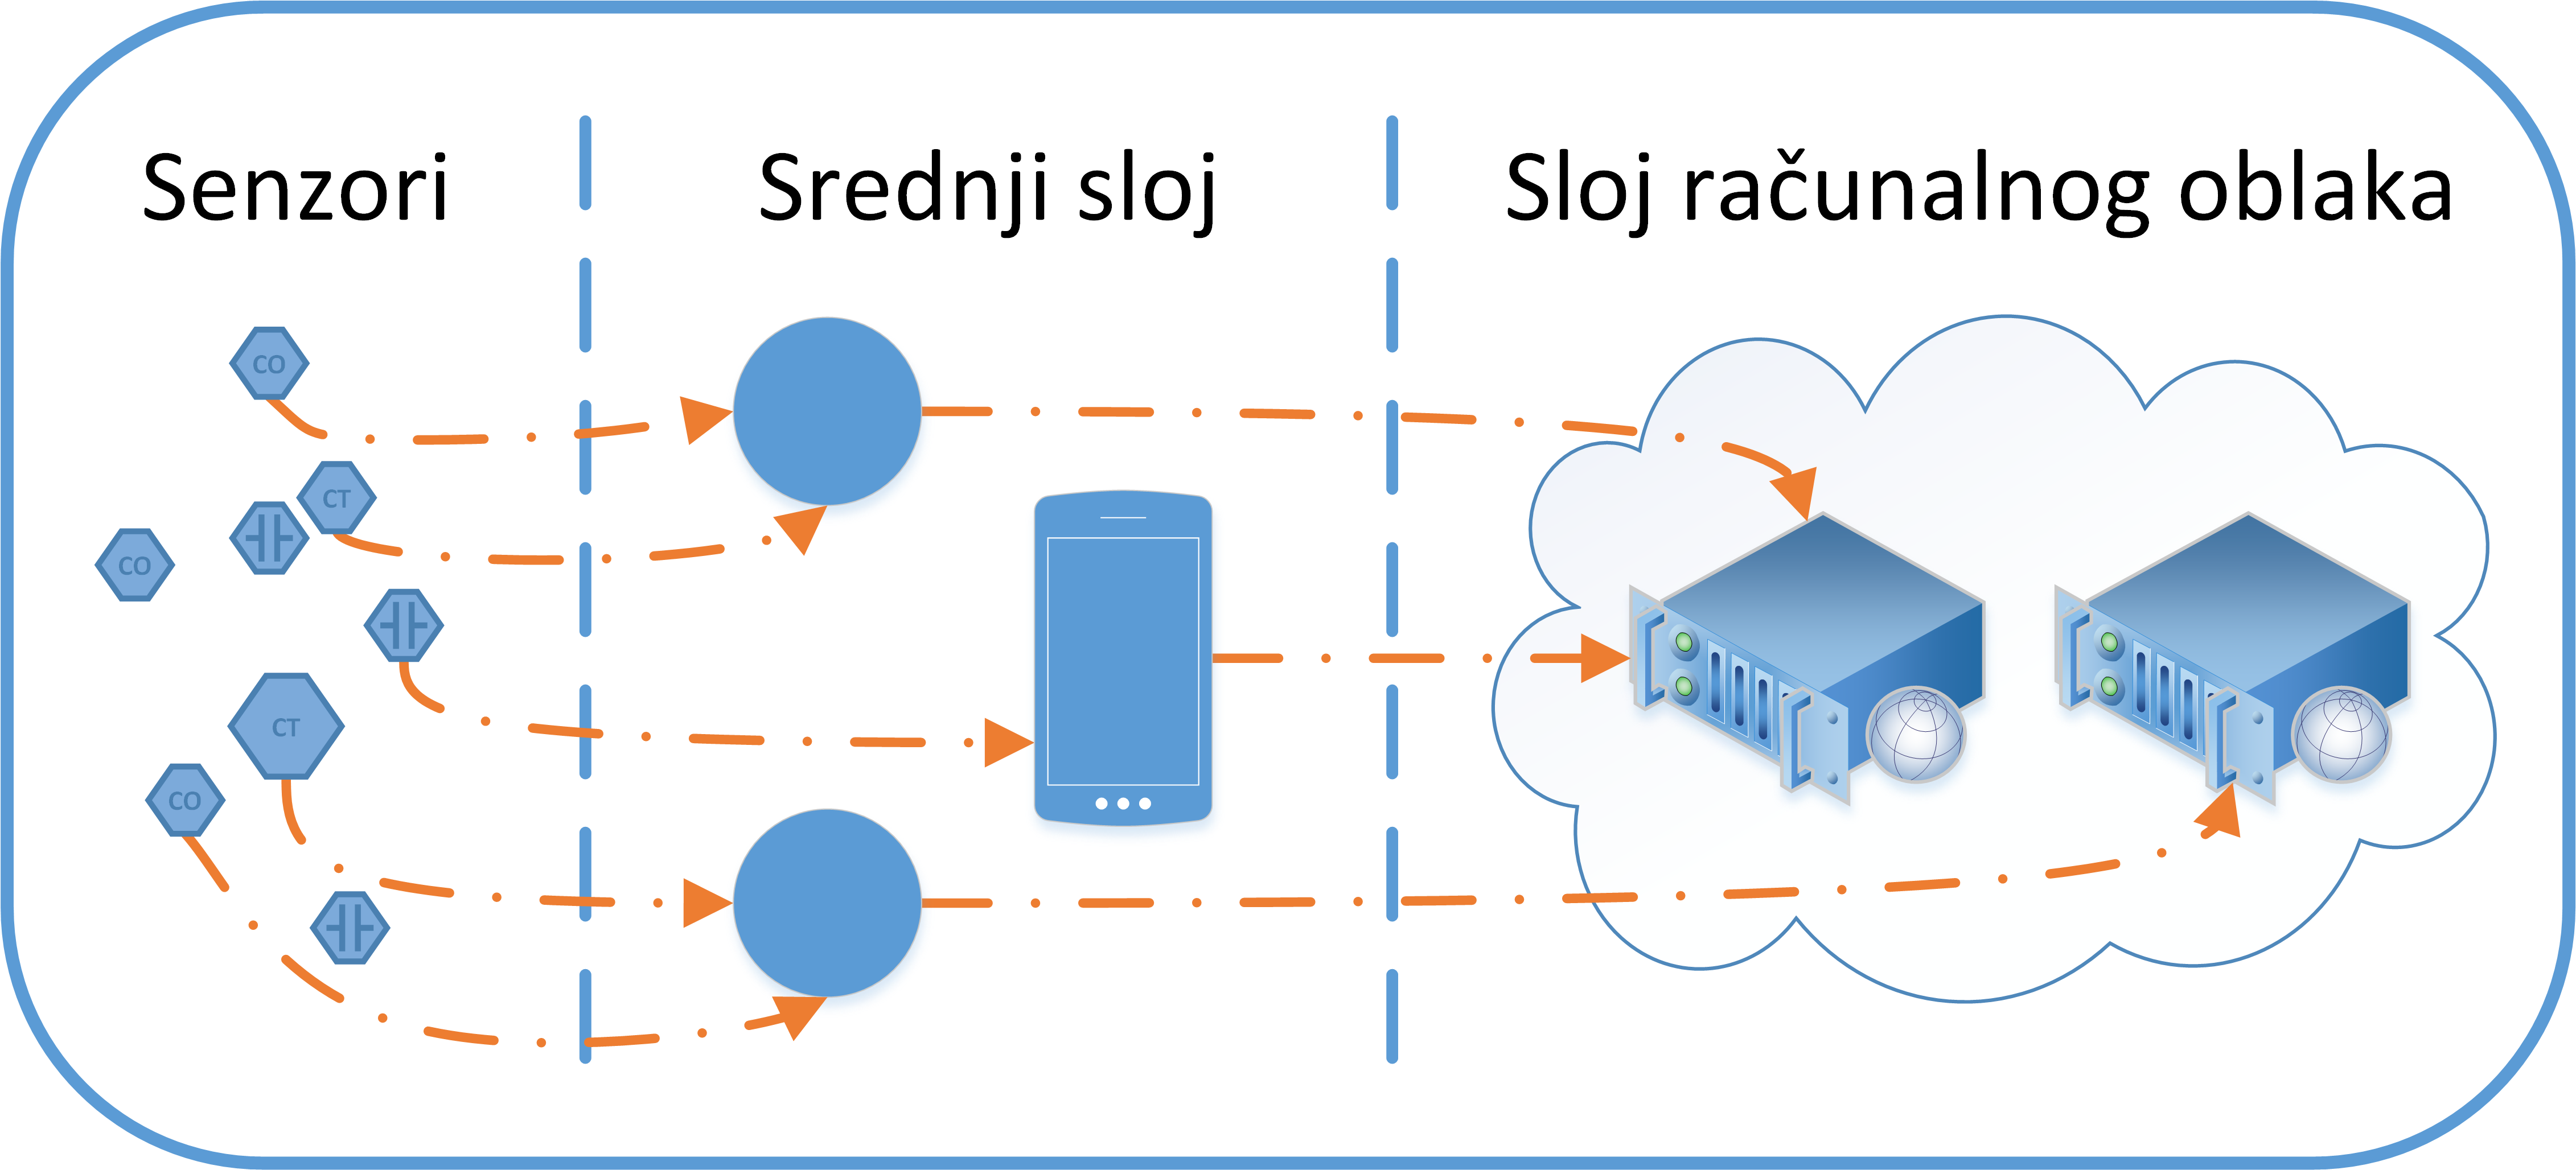
\includegraphics[width=\textwidth]{iot_reliable}
        \caption{Pouzdano prikupljanje podataka}
	\label{fig:reliable}
    \end{subfigure}
    \begin{subfigure}[b]{0.49\textwidth}
        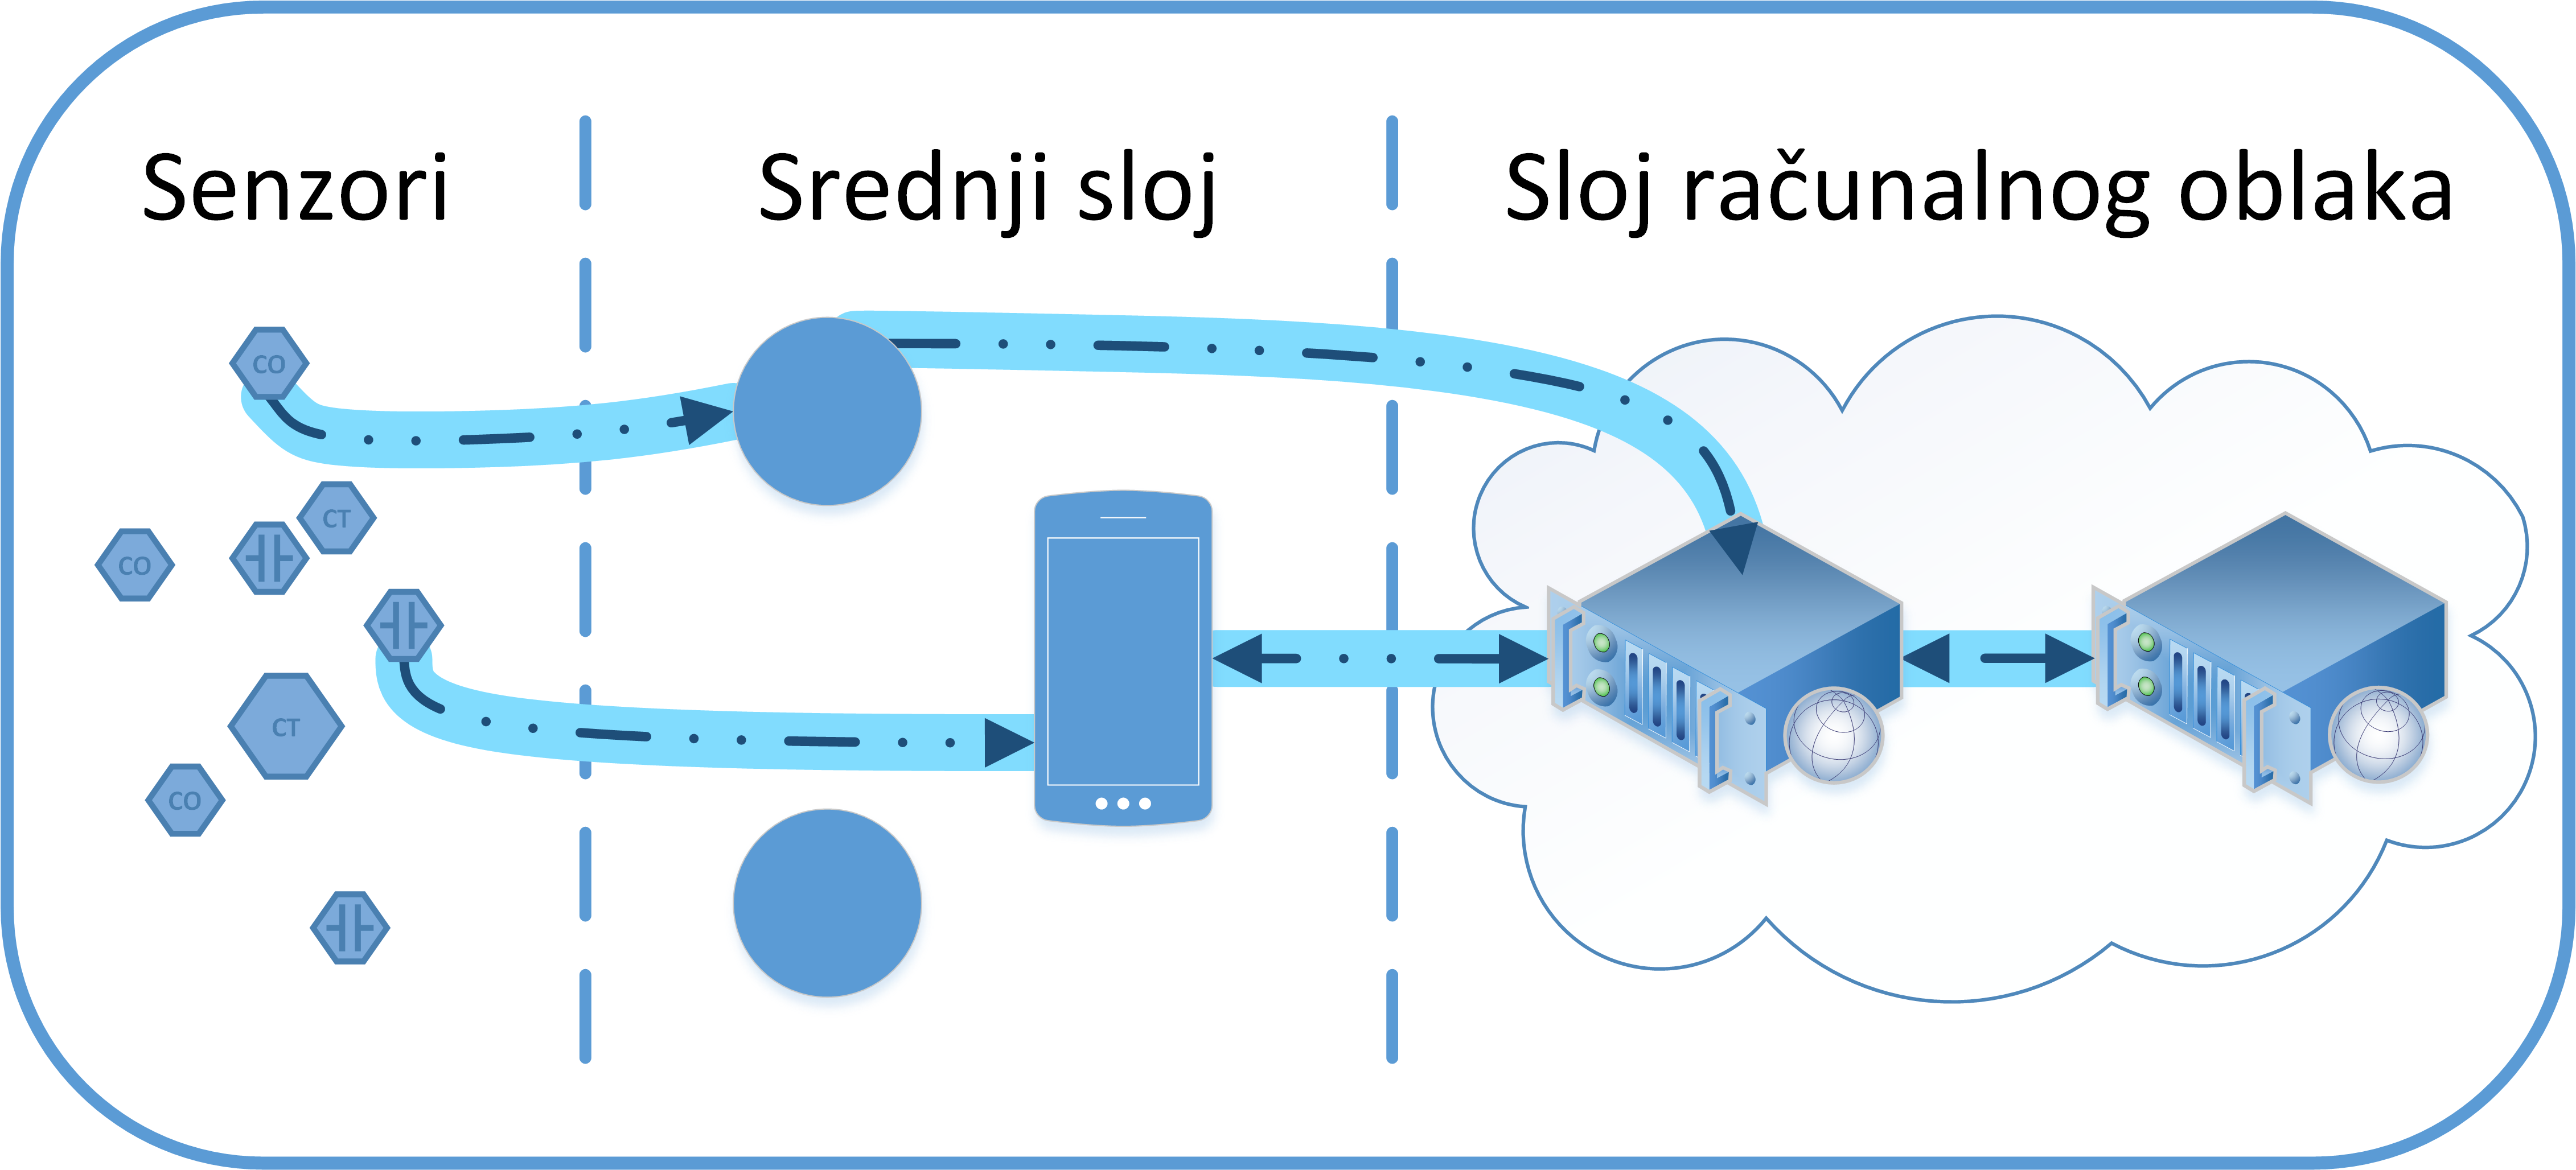
\includegraphics[width=\textwidth]{iot_sensitive}
        \caption{Zaštita osjetljivih podataka}
	\label{fig:sensitive}
    \end{subfigure}
    \caption{Primjene sigurne komunikacije u okolini Interneta stvari}
    \label{fig:iot}
\end{figure}

\subsection{Arhitektura neovisna o platformi} 
Neovisnost o platformi i uređajima u okolini Interneta stvari omogućena
je kroz uporabu prilagodljivog protokola ACAP za dogovor ključeva i algoritama koji
će se koristiti za zaštitu komunikacije. Protokol ACAP omogućuje dogovor u
oportunističkom mrežnom okruženju koje je karakteristično za Internet stvari i
podržava mogućnost dinamičke promjene kriptografskih algoritama i duljine
ključeva kako bi se ostvarila sigurnija komunikacija u slučaju ranjivosti ili
smanjilo opterećenje sustava u slučaju nedostatka resursa. Poruke u sustavu
mogu se razmjenjivati između dva uređaja ili biti proslijeđene od senzorskog
sloja sve do sloja računalnog oblaka, kako je prikazano na slici
\ref{fig:independent}. 

\subsection{Autentificirano upravljanje uređajima}
Svi uređaji, neovisno o sloju na kojem se nalaze, moraju imati sposobnost
autentifikacije kako bi se omogućilo pravilno upravljanje cijelog sustava
temeljenog na Internetu stvari. Upravljačke poruke obično dolaze iz sloja
računalnog oblaka i služe za prilagodbu uređaja u nižim slojevima arhitekture.
Tijek upravljačkih poruka prikazan je na slici \ref{fig:management}.
Autentifikacija upravljačkih poruka omogućava se tako da pošiljatelj
digitalno potpisuje poruke kako bi primatelj mogao provjeriti izvor poruke i
njenu cjelovitost. Digitalni potpis je računalno zahtjevna operacija i koristi
se samo za upravljačke poruke kako bi se uštedjelo na računalnim resursima.
Upravljačke poruke se, između ostalog, mogu koristiti za mijenjanje frekvencije
očitanja određenih senzora ili za slanje ažuriranja prema uređajima nižih
slojeva.

\subsection{Pouzdano prikupljanje podataka}
Uobičajeno je da se podaci prosljeđuju od izvora u nižim slojevima prema višim
slojevima. Tijekom prijenosa tih podataka napadač ima mogućnost presretanja
podataka i prosljeđivanja krivih mjerenja prema uređajima viših slojeva. To se
sprječava korištenjem HMAC zaštitne sume nad podacima koji se prosljeđuju. Time
je osigurana cjelovitost razmijenjenih poruka i omogućena pouzdanost
arhitekture. Pouzdani tok podataka za ovaj scenarij prikazan je na slici
\ref{fig:reliable}. Korištenje HMAC zaštitne sume umjesto digitalnog potpisa
omogućava značajno smanjenje složenosti operacija bez smanjivanja potrebne
razine sigurnosti (oba postupka omogućuju ostvarivanje sigurnosnog zahtjeva
cjelovitosti podataka). S obzirom na to da uređaji u sklopu senzorskog sloja imaju
pristup ograničenom izvoru napajanja, cilj je uštedjeti na potrošnji energije
prilikom zaštite podataka.
HMAC zaštita koristi se za prikupljanje podataka koji nisu osjetljivi (npr.
mjerenja kvalitete zraka ili vode), ali bi trebali biti vjerodostojni kako bi se
pružala kvalitetna usluga.

\subsection{Zaštita osjetljivih podataka}
U određenim scenarijima prikupljeni podaci mogu biti osjetljive prirode i
trebaju se zaštiti tako da sprječavaju curenje podataka kao što je prikazano
na slici \ref{fig:sensitive}. Potreba za zaštitom podataka može se pojaviti u
komunikaciji između svih slojeva u sklopu arhitekture. Iako senzori najčešće
prikupljaju neosjetljive podatke, određene primjene, poput sustava za
praćenje tjelesnog zdravlja, ne bi smjele dozvoljavati uvid u izmjerene podatke.
Isto tako, određene korporativne primjene zahtijevaju da svi podaci unutar
arhitekture budu tajni kako se ne bi otkrivali osjetljivi podaci o korisnicima
sustava. Zaštita osjetljivih podataka postiže se simetričnom kriptografijom,
odnosno šifriranjem podataka na izvoru i dešifriranjem na odredištu korištenjem
prethodno razmijenjenog tajnog ključa.

\section{Model sigurne komunikacije u okolini Interneta stvari}

Model sigurne komunikacije u okolini Interneta stvari definiran je kao šestorka
$S_{IoT}$:

\begin{equation}
    S_{IoT}=\{D,K,L,C,A,O\},
\end{equation}

gdje je $D$ skup svih uređaja (engl. \emph{devices}), $K$ skup svih parova
ključeva (privatnog i odgovarajućeg javnog ključa)
svih uređaja, $L$ je skup svih komunikacijskih slojeva (engl.
\emph{communication layers}) na kojem uređaji mogu komunicirati, $C$ skup svih
mogućnosti uređaja (engl. \emph{capabilities}), $A$ je skup kriptografskih
algoritama koje uređaji mogu koristiti i $O$ je skup operacija
s kojima se ostvaruje sigurna komunikacija između uređaja.

Za potrebe ovog modela razlikujemo tri različite vrste kriptografskih
algoritama u sklopu skupa $A=\{A^h,A^s,A^p\}$: algoritme kriptografskog sažetka
$A^h$, simetrične algoritme $A^s$ i asimetrične algoritme $A^p$.

Uređaj $D_i$ u modelu je označen sa svojim skupom podržanih
komunikacijskih slojeva $L_i$, skupom hardverskih mogućnosti $C_i$, skupom
podržanih kriptografskih algoritama $A_i$ i skupom parova javnih i privatnih
ključeva $K_i$:
\begin{equation}
    D_i \in D:\{D_i=\{L_i,C_i,A_i,K_i\},\ L_i \subseteq L,\ C_i \subset C,\ A_i 
    \subseteq A,\ K_i \subset K\},
\end{equation}
gdje je $A_i=\{A^h_i,A^s_i,A^p_i\}$ takav da vrijedi $A^h_i\subseteq A^h$,
$A^s_i\subseteq A^s$ i $A^p_i\subseteq A^p$.

Svaki par ključeva $k(a^p_i)\in K_i$ stvara se tako da odgovara asimetričnom
algoritmu $a^p_i\in A^p_i$. Par ključeva $k(a^p_i)$ 
sadrži privatni ključ $pri(a^p_i)$
i njemu odgovarajući javni ključ $pub(a^p_i)$:
\begin{equation}
    k(a^p_i)=\{pri(a^p_i), pub(a^p_i)\}.
\end{equation}

Skup javnih ključeva za svaki uređaj mora se prebaciti na drugi uređaj prilikom
uspostave sigurne komunikacije.
Skup javnih ključeva $PK_i$ za uređaj $D_i$ definiran je kao: 
\begin{equation}
PK_i=\{pub(a^p_i)\in k(a^p_i):k(a^p_i)\in K_i\}.
\end{equation}

U predloženom modelu, dva uređaja $D_i$ i $D_j$ mogu komunicirati samo
ako imaju zajednički komunikacijski sloj na kojem mogu komunicirati, odnosno ako
vrijedi sljedeće: $L_i \cap L_j \neq \emptyset$.
Komunikacijski sloj definira vrstu sučelja i mrežne protokole koji se mogu
koristiti za razmjenu podataka između uređaja (npr. WLAN, Ethernet, IP, TCP,
UDP). 

\no{
Note that a typical device from the perceptual 
tier has a wireless interface (e.g. Bluetooth or Zigbee) for interaction with a 
intermediate tier device, while the latter device uses a high speed communication 
interface (e.g. WLAN or Ethernet) to communicate with the cloud tier.
}

Za ostvarivanje sigurne komunikacije između uređaja u predloženom modelu
definira se skup operacija $O$ koji se sastoji od šest operacija namijenjenih
sigurnoj komunikaciji koje se koriste za dogovor algoritama i ključeva,
osiguravanje cjelovitosti podataka, autentifikaciju i tajnost podataka.
\begin{equation}
    O=\{dogovor, \mathit{potpis}, \mathit{provjera\_potpisa}, hmac, \mathit{sifriranje}, \mathit{desifriranje}\}
\end{equation}

Operacija dogovora kriptografskih algoritama i zajedničke tajne
(\textit{dogovor}) je preduvjet za daljnju sigurnu komunikaciju između
klijenta (započinjatelja) $D_i$ i poslužitelja (odgovaratelja) $D_j$ i mora biti
provedena prije svih drugih
operacija. Ova operacija dogovora predstavlja protokol ACAP koji služi za
dogovor oko preduvjeta sigurne komunikacije. Rezultat operacije je trojka
kriptografskih algoritama ($\widetilde{A}_{ij}$) koja se može koristiti na oba
uređaja, zajednička tajna ($S_{ij}$) koju se može koristiti za stvaranje novih
tajnih ključeva za zaštitu podataka i javni ključ svakog uređaja:
\begin{equation}
	dogovor:(D_i,D_j)\longmapsto\{\widetilde{A}_{ij},S_{ij},pub(a^p_i),pub(a^p_j)\},
	\label{eq:agreement}
\end{equation}
gdje vrijedi da je
$\widetilde{A}_{ij}=\{\widetilde{A}^h_{ij},\widetilde{A}^s_{ij},\widetilde{A}^p_{ij}\}$
takav da je $\widetilde{A}^h_{ij}\in A^h_{i}\cap A^h_{j}$,
$\widetilde{A}^s_{ij}\in A^s_{i}\cap A^s_{j}$ i $\widetilde{A}^p_{ij}\in
A^p_{i}\cap A^p_{j}$. 

Drugim riječima, dogovoreni algoritmi kriptografskog sažetka, simetrične i
asimetrične kriptografije moraju biti podržani na oba uređaja.
Javni ključevi $pub(a^p_i)$ i $pub(a^p_j)$ odgovaraju dogovorenom algoritmu
asimetrične kriptografije $\widetilde{A}^p_{ij}$ tako da vrijedi
$a^p_i=a^p_j=\widetilde{A}^p_{ij}$. Do zajedničke tajne $S_{ij}$ dolazi se s
pomoću Diffie-Hellman izračuna opisanog u poglavlju \ref{sec:dh}.


U modelu definirane su sljedeće sigurne komunikacijske operacije koje se
mogu izvoditi samo nakon uspješne operacije dogovora:
\begin{itemize}  
    \item Zaštita cjelovitosti podataka uz neporecivost (\textit{potpis}) u obliku
	digitalnog potpisa za podatke koje se razmjenjuju između pošiljatelja
	$D_i$ i primatelja $D_j$:
	\begin{equation}
	    \mathit{potpis}:[podaci,\widetilde{A}^h_{ij},\widetilde{A}^p_{ij},pri(a^p_i)]\longmapsto\{\mathit{digitalni\_potpis}\}.
	    \label{eq:sign}
	\end{equation}
	    
	Digitalni potpis računa se iz podataka kroz izračun
	kriptografskog sažetka dogovorenim algoritmom $\widetilde{A}^h_{ij}$ te
	asimetričnom operacijom potpisivanja korištenjem algoritma
	$a^p_i=\widetilde{A}^p_{ij}$ i odgovarajućeg privatnog ključa
	$pri(a^p_i)$. Uređaj $D_j$ po primitku podataka provjerava valjanost
	digitalnog potpisa korištenjem operacije $provjera\_potpisa$:
	\begin{equation}
	    \mathit{provjera\_potpisa}:[\{podaci,\mathit{potpis}\},\widetilde{A}^h_{ij},\widetilde{A}^p_{ij},pub(a^p_i)]\longmapsto~[ispravan,neispravan]
	\end{equation}
	Primatelj $D_j$ provjerava dobiveni digitalni potpis tako
	da uspoređuje rezultat kriptografskog sažetka s algoritmom
	$\widetilde{A}^h_{ij}$ nad dobivenim podacima,
	s dešifriranim kriptografskim sažetkom iz digitalnog potpisa
	algoritmom $a^p_j=\widetilde{A}^p_{ij}$ i odgovarajućim
	javnim ključem $pub(a^p_i)$. Ako se sažeci podudaraju potpis je
	ispravan, u suprotnom potpis je neispravan.

    \item Autentifikacija podataka i zaštita cjelovitosti algoritmom HMAC
	(\textit{hmac}) koristi se kao jednostavniji mehanizam zaštite koji
	zahtijeva manje resursa od digitalnog potpisa. Operacija \emph{hmac}
	prilikom slanja podataka $data$ između pošiljatelja $D_i$ i primatelja
	$D_j$ definirana je na sljedeći način:
	\begin{equation}
	    hmac:(podaci,\widetilde{A}^h_{ij},S_{ij})\longmapsto\{za\breve{s}titna\_suma\}
	    \label{eq:hmac}
	\end{equation}
	
	Zaštitna suma se računa korištenjem dogovorenog algoritma kriptografskog
	sažetka $\widetilde{A}^h_{ij}$ s dogovorenom zajedničkom tajnom $S_{ij}$
	nad podacima koji se šalju.
	Primatelj $D_j$ uspoređuje dobivenu zaštitnu sumu sa zaštitnom sumom
	izračunatom nad dobivenim podacima s istim ključem. Provjera zaštitne
	sume je uspješna ako se primljena i izračunata zaštitna suma podudaraju.
	
    \item Tajnost podataka korištenjem operacija \textit{sifriranje} i
	\textit{desifriranje} za podatke razmijenjene između pošiljatelja $D_i$
	i primatelja $D_j$. Operacija šifriranja koristi prethodno dogovoreni
	algoritam simetrične kriptografije $\widetilde{A}^s_{ij}$ i zajedničku
	tajnu $S_{ij}$ nad podacima:
	\begin{equation}
	    \mathit{sifriranje}:(podaci,\widetilde{A}^s_{ij},S_{ij})\longmapsto~\mathit{tajni\_podaci}
	\end{equation}
	Izvorni podaci se izračunavaju s operacijom dešifriranja uz korištenje
	istog algoritma i zajedničke tajne:
	\begin{equation}
	    \mathit{desifriranje}:(\mathit{tajni\_podaci},\widetilde{A}^s_{ij},S_{ij})\longmapsto~podaci
	\end{equation}
\end{itemize}

Predstavljeni model sigurne komunikacije je minimalan skup objekata i operacija
koje su potrebne za sigurnu komunikaciju između svih uređaja unutar okoline
Interneta stvari neovisno o njihovim mogućnostima.

\section{Prilagodljivost modela sigurne komunikacije}
\label{sec:iotprilag}

Predloženi model je prilagodljiv jer podržava različite načine dogovora
korištenih algoritama ovisno o trenutnim mogućnostima uređaja $D_i$ i $D_j$. Za
odabir algoritama koristi se poopćenje procedure koja je definirana u poglavlju
\ref{sec:dogovor}, a temeljeno je na protokolu SSH \ref{sec:ssh}. Protokol SSH
uzima u
obzir samo redoslijed algoritama u popisu, odnosno pretpostavlja da će
algoritmi biti poredani po sigurnosti ili brzini izvođenja. Osnovni
nedostatak tog pristupa je nemogućnost dinamičke promjene uvjeta odabira.

\no{Predložena procedura je poopćena inačica postupka koji se koristi u sklopu protokola SSH prikazanog u poglavlju \ref{sec:ssh}. Protokol SSH pretpostavlja najvišu razinu sigurnosti i ne uzima u obzir računalne sposobnosti komunicirajućih strana. Ukoliko je kriptografski algoritam implementiran, on će se koristiti neovisno o mogućem utjecaju na brzinu obrade zaštićenih podataka.}

Za područje Interneta stvari prikladan je unaprijeđeni algoritam dogovora koji je
prikazan u algoritmu \ref{alg:agreement2}, a omogućuje dinamičko
odlučivanje oko algoritma koji će se koristiti ovisno o trenutnim sposobnostima
komunicirajućih strana.
Osnova za vrednovanje algoritama leži u odlučivanju koji je algoritam
primjereniji za upotrebu ovisno o uvjetima u kojima se odvija sigurna
komunikacija. Vrijednost algoritma može biti povezana izravno s mjerljivim
mogućnostima komunicirajućih uređaja, poput računalne moći, propusnosti
komunikacije ili pristupa izvoru napajanja.

\begin{algorithm}
\caption{Procedura za dogovor kriptografskih algoritama}
\label{alg:agreement2}
\begin{algorithmic}[1]
    \Procedure{Crypto\textendash Agreement}{$C_i$, $C_j$, $A_i$, $A_j$, $rsig$}\
    \For{svaka $vrsta \in \{h,s,p\}$}
    \For{svaki $a^{vrsta} \in (A^{vrsta}_i \cap A^{vrsta}_j)$}
    \If{($\widetilde{A}^{vrsta}_{ij} == \varnothing$) \textbf{or} 
    $(score(a^{vrsta},C_i,C_j,rsig) > score(\widetilde{A}^{vrsta}_{ij},C_i,C_j, rsig))$}
		\State $\widetilde{A}^{vrsta}_{ij}$ = $a^{vrsta}$
		\State \textbf{break}
	    \EndIf
	\EndFor
	\If{$\widetilde{A}^{vrsta}_{ij} == \varnothing$}
	\State \Return $\varnothing$ \Comment Dogovor je neuspješan jer nema zajedničkih algoritama.
	\EndIf
    \EndFor
    \State \Return 
    $\widetilde{A}_{ij}=\{\widetilde{A}^{h}_{ij},\widetilde{A}^{s}_{ij},\widetilde{A}^{a}_{ij}\}$
\EndProcedure
\end{algorithmic}
\end{algorithm}

Algoritam uzima u obzir mogućnosti klijenta i poslužitelja $C_i$ i $C_j$ te
potrebnu razinu sigurnosti $rsig$ kako bi iz popisa podržanih algoritama
$A_i$ i $A_j$ odabrao prikladne algoritme ovisno o trenutnim mogućnostima (linija 1).

Procedura dogovora prolazi kroz sve vrste algoritama koje su potrebne za
osiguravanje daljnje komunikacije (hash - $h$ , simetrični - $s$, asimetrični - $p$)
(linija 2-12) i za svaku vrstu odabire algoritam $a^{vrsta}$ iz presjeka
algoritama obje strane ($A^{vrsta}_i \cap A^{vrsta}_j$). Odabire se algoritam
koji ima najveću
vrijednost u odnosu na ostale algoritme (linije 3-8). Vrijednost pojedinog
algoritma određuje
se s pomoću funkcije za računanje vrijednosti $score(a^{vrsta},C_i,C_j,rsig)$
(linija 4). Konačno, procedura vraća n-torku odabranih algoritama (linija 13)
ili prazan skup (linija 10) koji predstavlja neuspješan dogovor. Predložena
procedura za dogovor je ostvarena uz pretpostavku da je razina sigurnosti
najvažniji parametar. U tom slučaju se ova procedura može poistovjetiti s
procedurom za odabir u protokolu SSH.

Prilikom postavljanja cjelokupne okoline za sigurnu komunikaciju potrebno je
izmjeriti podatke o mogućnostima uređaja koji sudjeluju u komunikaciji i prema
tome odrediti parametre za funkciju vrednovanja $score$.
Funkcija $score$ za vrednovanje algoritama omogućuje fleksibilno definiranje
vrijednosti ovisno o pojedinoj primjeni. U okolini Interneta stvari važno je
uzeti u obzir trenutne mogućnosti uređaja i prema tome odrediti koji je
algoritam najbolji, a koji najgori u danom trenutku. Ukupna vrijednost algoritma
$a$, koja je definirana izrazom $score(a,C_i,C_j,rsig)$, zapravo je
kombinacija vrijednosti u više dimenzija. Osnovne dimenzije dolaze od trenutno
zahtjevane razine sigurnosti $rsig$, računalne zahtjevnosti algoritma $ac$
(engl. \emph{algorithm complexity}) i trenutnih mogućnosti oba uređaja koje
obuhvaćaju trenutnu razinu napajanja $bp$ (engl. \emph{battery power}),
propusnosti komunikacijske veze $bw$ (engl. \emph{bandwidth}) i računalne snage
uređaja $pp$ (engl. \emph{processing power}):
\vspace{-10pt}
\begin{multline}
    score(a,C_i,C_j,rsig)=\\f[w_{0}\cdot rsig, w_{1}\cdot ac(a), 
	w_{2}\cdot min(bp_i,bp_j), 
    w_{3}\cdot min(bw_i,bw_j), w_{4}\cdot min(pp_i,pp_j)],
\end{multline}
gdje su $C_i$ i $C_j$ redom definirani kao $\{bp_i,bw_i,pp_i\}$ i
$\{bp_j,bw_j,pp_j\}$. Različite težine $w_x$ ukazuju na relativnu važnost
i definiraju doprinos određene dimenzije u odnosu na cjelokupnu vrijednost
algoritma. Odnosi težina se određuju na temelju trenutne primjene i okoline u
kojoj je sustav postavljen. Prioritet se daje uređaju koji trenutno ima manju
razinu mogućnosti (funkcija $\min$).

\subsection{Prilagodbe odabira algoritma}

Funkcija za vrednovanje $score$ omogućuje prilagodljivost procedure za dogovor
na razne uvjete komunikacije ovisno o namjeni i ograničenjima sustava.
Primjerice:
\begin{itemize}
    \item Ako se radi o sustavu koji prikuplja i obrađuje velike količine
	podataka, najveća težina će se postaviti na propusnost komunikacijske
	veze $bw_x$ i na računalnu zahtjevnost algoritma $ac_x$ kako se podaci
	mogli sigurno prikupljati zavodoljavajućom brzinom.
    \item U slučaju postavljanja sustava za dugoročno prikupljanje, težina će
	biti postavljena na trenutnu razinu napajanja $bw_x$.
    \item Kod postavljanja sustava s visokim zahtjevima na sigurnost, težina će
	se postaviti na razinu sigurnosti komunikacije $rsig$, a drugi ključni
	parametar će biti računalna snaga uređaja $pp_x$.
\end{itemize}

Prilikom specifikacije funkcije vrednovanja važno je odrediti što je prioritet
kod postavljanja sustava. U slučaju da imamo sustav za prikupljanje podataka o
temperaturi na određenom području, važno je odrediti kroz koji će se period
prikupljati očitanja i procijeniti trošak obrade pojedinog mjerenja koji
uključuje mjerenje, zaštitu podataka i slanje podataka. Različiti algoritmi
će imati različitu zahtjevnost, odnosno potrošnju električne energije. Stoga je
važno pravilno izmjeriti težinu pojedinog algoritma za uređaj koji se postavlja
i definirati računalne zahtjevnosti za svaki algoritam.

Ako se za vrijeme rada sustava promijene zahtjevi na sigurnost ili se postave
drukčiji prioriteti na težinu određenih parametara, moguće je s viših slojeva
ažurirati težine tih parametara i prilagoditi sustav trenutnim potrebama. Na taj
način bi se mogla smanjiti učestalost očitanja kako bi se uštedjela energija
potrebna za omogućavanje tajnosti očitanih podataka.

Prilikom komunikacije dva uređaja s različitih slojeva, prioritet kod izračunavanja
funkcije vrednovanja daje se uređaju koji se nalazi na nižem sloju arhitekture.
Na taj se način štede resursi u nižim slojevima arhitekture kako bi se
prikupljanje podataka obavilo na što efikasniji način.

% vim: spell spelllang=hr

\chapter{Programsko ostvarenje protokola ACAP}
\label{ch:impl}

Programsko ostvarenje ACAP izvedeno je u programskom jeziku Python 3 koji
koristi dodatne biblioteke za kriptografiju
(pycrypto\footnote{https://www.dlitz.net/software/pycrypto/} i
cryptography\footnote{https://cryptography.io/en/latest/}) i biblioteku za
prepoznavanje mrežnih sučelja za
potrebe rada na sloju Ethernet
(netifaces\footnote{https://pypi.python.org/pypi/netifaces}). Programsko
ostvarenje podržava
pokretanje aplikacije u klijentskom i poslužiteljskom načinu rada i kao rezultat
vraća sljedeće podatke:
\begin{itemize}
\item popis dogovorenih algoritama razvrstanih u kategorije,
\item tajni ključ koji se može koristiti za osiguravanje tajnosti korištenjem
simetričnih algoritama šifriranja i dešifriranja ili osiguravanje
cjelovitosti korištenjem algoritma HMAC i
\item javni ključ druge strane koji se može koristiti za provjeru identiteta i
osiguravanje cjelovitosti korištenjem digitalnog potpisa.
\end{itemize}

U ovom poglavlju objašnjen je način rada ostvarenja protokola
ACAP kroz pokretanje na različitim mrežnim slojevima i prikaz strukture poruka.
Nakon toga dana je analiza performansi uz mjerenja koja prikazuju složenost
kriptografskih operacija. Na kraju poglavlja prikazani su ugrađeni sigurnosni
mehanizmi. Aktualna verzija programskog ostvarenja uz upute za instalaciju može se
dohvatiti sa sljedeće poveznice:
\begin{center}
    \url{http://public.tel.fer.hr/acap}
\end{center}

\section{Arhitektura programskog ostvarenja i načini integracije}
Protokol ACAP sastoji se od sljedećih sastavnih dijelova:
\begin{itemize}
    \item izračun i provjera kriptografskih algoritama,
    \item obrada poruka,
    \item komunikacija neovisna o sloju,
    \item dogovor kriptografskih algoritama i
    \item komunikacija s vanjskim aplikacijama.
\end{itemize}

Cjelokupna arhitektura programskog ostvarenja prikazana je na slici \ref{fig:impl}.
Nakon što protokol ACAP zaprimi zahtjev za dogovorom kriptografskih algoritama
kroz sustav za komunikaciju s vanjskim aplikacijama, pokreće se proces dogovora
algoritama i ključeva prema ACAP poslužitelju na drugoj strani. U dogovoru se
međusobno izmjenjuju sustavi za izračun i provjeru kriptografskih algoritama,
obradu poruka te slanje i primanje paketa. Na kraju dogovora
pokreće se sustav za dogovor algoritma koji daje popis dogovorenih algoritama,
na temelju kojih se generira dogovorena duljina kriptografskog ključa uz pomoć
funkcije za generiranje nasumičnih vrijednosti. Na kraju
se popis dogovorenih algoritama zajedno s kriptografskim ključevima šalje
aplikaciji koja je pokrenula dogovor. Nakon ACAP razmjene pozivajuća aplikacija
može sigurno komunicirati korištenjem dogovorenih algoritama i ključeva.

\begin{figure}[htb]
    \centering
    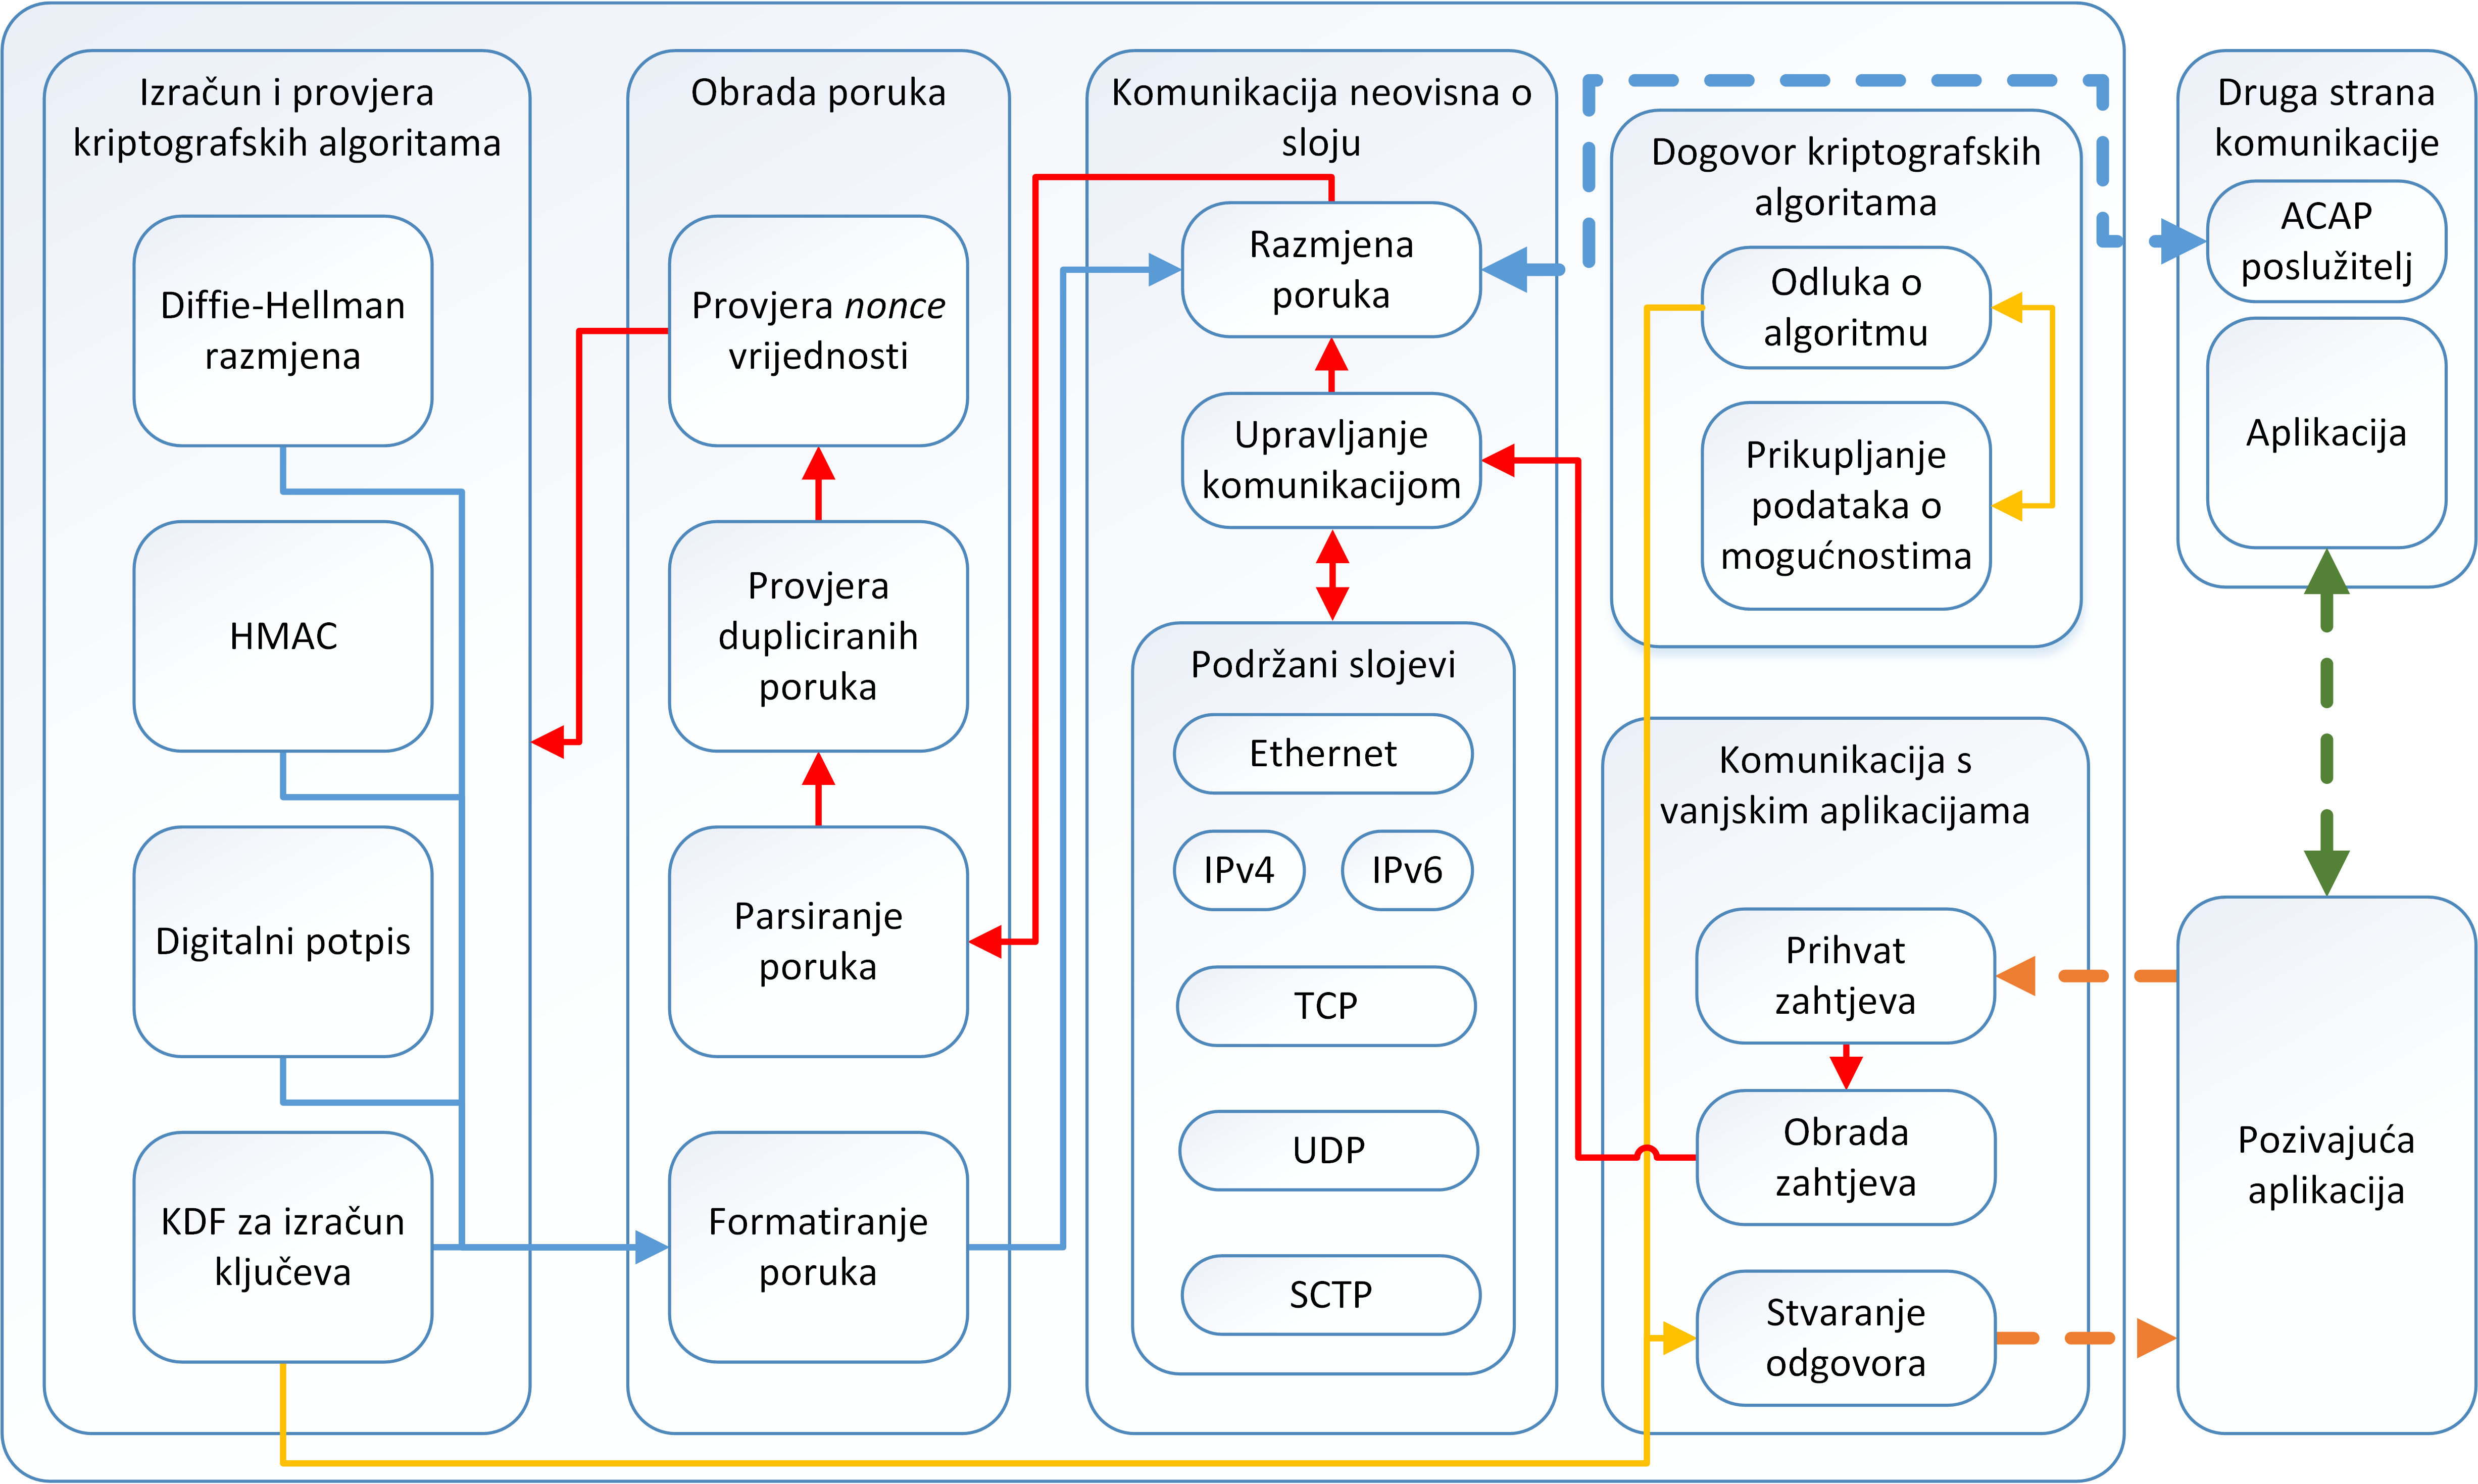
\includegraphics[width=0.98\textwidth]{arhitektura}
    \caption{Arhitektura programskog ostvarenja protokola ACAP}
    \label{fig:impl}
\end{figure}

Programsko ostvarenje protokola ACAP izravno podržava primjenu u sklopu modela
klijent-poslužitelj.
Primjena u mrežama ravnopravnih čvorova
postiže se pokretanjem poslužitelja na svim čvorovima u mreži te se dogovor
algoritama i ključeva odvija u parovima čvorova. Na taj način omogućeno je da
komunikacija između svaka dva čvora u mreži dobije razinu zaštite komunikacije
koja je primjerena mogućnostima tih čvorova. Grupni dogovor ključeva i
algoritama između ravnopravnih čvorova nije omogućen jer bi to nužno smanjivalo
razinu sigurnosti na mogućnosti najslabijeg čvora i omogućilo napadaču
razne napade na sigurnost samog protokola.

\section{Mogućnosti programskog ostvarenja}
Prilikom pokretanja ostvarenja moguće je specificirati hoće li se pokrenuti
poslužiteljska ili klijentska instanca protokola. U slučaju klijentske strane
potrebno je definirati adresu poslužitelja. Nadalje, može se specificirati koji
se protokol želi koristiti za prijenos poruka. Moguće je odabrati između
protokola TCP, SCTP, UDP, IP i Ethernet. Dodatno, za protokole TCP,
SCTP, UDP i IP moguće je koristiti protokol IP verzije 4 i protokol IP verzije 6.
Pretpostavljene opcije prilikom pokretanja su korištenje protokola TCP s IPv4
adresama za transport, korištenje standardnog Diffie-Hellman postupka i
algoritma RSA za digitalno potpisivanje.

Za osnovno pokretanje potrebno je definirati želi li se pokrenuti poslužitelj
ili klijent. Za pokretanje poslužitelja koristi se opcija "\texttt{-S}", a za
pokretanje klijenta opcija "\texttt{-C}". Potrebno je definirati popis podržanih
algoritama s opcijom "\texttt{-a}", u suprotnom će se popis algoritama
automatski dohvatiti iz trenutno dostupnih kriptografskih algoritama u sustavu.
Nužno je još definirati privatni ključ s pomoću opcije "\texttt{-k}", koja uzima
datoteku s RSA privatnim ključem veličine barem 768 okteta. Iz tog
privatnog ključa dobiva se javni ključ koji služi za identifikaciju tijekom
razmjene. Rezultati uspješne razmjene prikazani su na slikama
\ref{fig:acap_client} i \ref{fig:acap_server}.

Na slici \ref{fig:acap_client} vidi se skraćeni ispis pokretanja klijenta kojemu
je potrebno dodatno definirati adresu poslužitelja na koju će se spojiti
("\texttt{-h 10.0.0.20}"). Nakon
razmjene poruka klijent dobiva javni ključ poslužitelja, popis
dogovorenih algoritama i dijeljenu zajedničku tajnu. Na kraju ispisa prikazano
je ukupno trajanje dogovora od početka razmjene. Potpuni ispis klijenta sa svim
ključevima moguće je vidjeti u dodatku \ref{app:cli_impl}.

\begin{figure}[htb]
\begin{footnotesize}
\begin{verbatim}
$ ./acap.py -C -a client.json -k private_key_client -h 10.0.0.20
INFO - Server public key: -----BEGIN PUBLIC KEY-----
MIGfMA0GCSqGSIb3DQEBAQUAA4GNADCBiQKBgQCTYB3xU17CS5AGxKbWraxuGOYb
7sff8AAjjiwXrdBr6jqJ5zSHtR/bKxsRNPMNvzihVI1Taa7/CQy3EIRKkLeG4I7M
USeStpBfvQlpAK+lmyUE3haXVUNgPpALdXUpn+IaB+TDHuWl19z9dPDkSDLzQzga
pVwSgXpEZDUInwKK4QIDAQAB  -----END PUBLIC KEY-----
INFO - Client negotiated: 
{  "hash": {
        "algorithm": "SHA-256",
        "timestamp": "2015-11-22 14:59" },
    "public_key": {
        "algorithm": "RSA_2048",
        "timestamp": "2015-11-22 14:59" },
    "secret_key": {
        "algorithm": "AES-CTR_256",
        "timestamp": "2015-11-22 14:59" } }
INFO - Shared secret key (256 bit): bb:66:cc:98:10:fd:b7:a0:73:9b:9e:35:49:11:
43:7e:e5:28:3d:b3:69:5e:e2:69:4c:c9:a8:11:6d:d5:57:9a
INFO - TOTAL duration: 119820
\end{verbatim}
\end{footnotesize}
\vspace{-15pt}
\caption{Primjer pokretanja ACAP klijenta}
\label{fig:acap_client}
\end{figure}

Na slici \ref{fig:acap_server} prikazan je skraćeni ispis sa strane
poslužitelja.
Jedina značajna razlika vidljiva je u prvoj liniji koja označava da
su osvježene vrijednosti Diffie-Hellman eksponenta i poslužiteljski \emph{nonce}
("\texttt{Refreshed DH and Nonce...}"). Taj se proces kod poslužitelja odvija u
pozadini i služi za smanjenje utjecaja DoS napada na protokol ACAP na način
opisan u poglavlju \ref{sec:sigurnost}. Potpuni prikaz poslužitelja sa svim
ključevima prikazan je u dodatku \ref{app:serv_impl}.

\begin{figure}[htb]
\begin{footnotesize}
\begin{verbatim}
$ ./acap.py -S -a server.json -k private_key_server
Refreshed DH and Nonce...
INFO - Client public key: -----BEGIN PUBLIC KEY-----
MIGfMA0GCSqGSIb3DQEBAQUAA4GNADCBiQKBgQC4TDSclGnCkXgP0C8mt889rBRl
iFoXBtOlG4VF1XxhxursgU+Es2PCqRUYT28ZqdNrq2CAyuIT33G5CXCwg8x/CBh2
qmFJ43NpauGg13b2LFNSg3j8UxxwGSGIvKvxOmaGnSJByepogXkWuY0bL5mR0n0l
JPH/imO5V2+Jox951QIDAQAB  -----END PUBLIC KEY-----
INFO - Server negotiated: 
{   "hash": {
        "algorithm": "SHA-256",
        "timestamp": "2015-11-22 14:59" },
    "public_key": {
        "algorithm": "RSA_2048",
        "timestamp": "2015-11-22 14:59" },
    "secret_key": {
        "algorithm": "AES-CTR_256",
        "timestamp": "2015-11-22 14:59" } }
INFO - Shared secret key (256 bit): bb:66:cc:98:10:fd:b7:a0:73:9b:9e:35:49:11
:43:7e:e5:28:3d:b3:69:5e:e2:69:4c:c9:a8:11:6d:d5:57:9a
INFO - TOTAL duration: 17757
\end{verbatim}
\end{footnotesize}
\vspace{-15pt}
\caption{Primjer pokretanja ACAP poslužitelja}
\label{fig:acap_server}
\end{figure}

Prilikom pokretanja moguće je odabrati kriptografske algoritme koji se
zasnivaju na korištenju eliptičkih krivulja. To se radi s pomoću opcije
"\texttt{-E}" koja specificira da se umjesto standardnog Diffie-Hellman postupka
koristi ECDH (engl. \emph{Elliptic Curve Diffie-Hellman}) te da se umjesto
algoritma RSA koristi algoritam ECDSA za digitalno potpisivanje. Tada se
umjesto privatnog RSA ključa mora specificirati ECDSA privatni ključ.

\comment{lokalna baza s rezultatom dogovora, prvo implementirati, pa onda prikazati}

\section{Struktura poruka}

Poruke koje se razmjenjuju u protokolu ACAP prikazane su u poglavlju
\ref{sec:poruke}. S obzirom na to da su osnovni dijelovi tih poruka varijabilne
duljine, prije svakog od tih dijelova dodano je polje koje označava duljinu
parametra. Bitovni zapis poruke \initi{} prikazan je na slici \ref{fig:initi_fmt}. Za
definiranje svih duljina koriste se dva okteta koja sadrže duljinu polja
izraženu u broju okteta. Formati ostalih poruka nalaze se u dodatku
\ref{app:formats}.

\begin{figure}[htb]
    \centering
\begin{bytefield}[bitwidth=0.75em]{32}
\bitheader{0,7,15,23,31} \\
\bitbox{16}{\colorbox{blue!30}{Duljina poruke}} & \bitbox{8}{\colorbox{red!30}{Tip=0}} & \bitbox{8}{\colorbox{yellow!30}{Duljina DH}} \\
\bitbox{8}{\colorbox{yellow!30}{Duljina DH}} & \bitbox[lr]{24}{} \\
\wordbox[lr]{2}{\colorbox{orange!30}{Klijentov Diffie-Hellman javni dio} \\ $\vdots$} \\
\bitbox{16}{\colorbox{green!30}{Duljina \emph{noncea}}} & \bitbox[lrt]{16}{} \\
\wordbox[lrb]{2}{\colorbox{purple!30}{Klijentov \emph{nonce}} \\ $\vdots$}
\end{bytefield}
\caption{Bitovni zapis poruke \initi{}}
\label{fig:initi_fmt}
\end{figure}

Na slici \ref{fig:initi_bits} dan je bitovni prikaz jedne poruke \initi{} koji je
obojan u skladu s bitovnim zapisom iz slike \ref{fig:initi_fmt} kako bi se lakše
identificirala polja poruke. Na početku se nalazi duljina poruke u oktetima
(\texttt{0x0091}=145), potom je naveden tip poruke (\texttt{0x00}), a zatim
duljina DH javnog dijela klijenta (\texttt{0x0080}=128) i vrijednost DH javnog
dijela. Na samom kraju poruke
zapisana je duljina klijentovog \emph{noncea} (\texttt{0x000c}=12) i vrijednost
\emph{noncea}.
Cjelokupna duljina poruke jednaka je zbroju duljina svih navedenih dijelova
($1+2+128+2+12=145$).

\begin{figure}[htb]
\begin{center}
\begin{minipage}{0.6\linewidth}
\begin{footnotesize}
\begin{monoblock}
\noindent 0x00:\colorbox{blue!30}{00 91}\colorbox{red!30}{00}\colorbox{yellow!30}{00 80}\colorbox{orange!30}{27 2d d0 e9 6a f9 d7 37 2e a1 c8} \\
0x10:\colorbox{orange!30}{6c 23 0a c9 44 98 13 c6 ed 27 fc ac b8 3c 91 dc} \\
0x20:\colorbox{orange!30}{82 4a 1d f0 af 47 5a 87 63 42 24 0b e4 2b e1 0f} \\
0x30:\colorbox{orange!30}{e0 1f fa 54 c6 14 5d 4f bf 13 c6 76 70 5f 65 06} \\
0x40:\colorbox{orange!30}{8d 74 c6 1f 9f 1f 00 dd 71 55 65 d3 09 44 da 59} \\
0x50:\colorbox{orange!30}{cf 37 74 e1 f1 b3 38 55 38 51 20 b9 25 c8 68 b0} \\
0x60:\colorbox{orange!30}{03 cd e0 dd 97 34 ab 99 3e 75 36 c2 8f 78 fd b9} \\
0x70:\colorbox{orange!30}{9e a5 7e df bc ee ea 50 d0 f0 8e ce 4d 02 e8 75} \\
0x80:\colorbox{orange!30}{b5 9b 5e 62 d7}\colorbox{green!30}{00 0c}\colorbox{purple!30}{c7 48 6b 13 6f d8 16 e0 00} \\
0x90:\colorbox{purple!30}{15 ce 6b}
\end{monoblock}
\end{footnotesize}
\end{minipage}
\vspace{-20pt}
\end{center}
\caption{Bitovni prikaz primjera poruke \initi{}}
\label{fig:initi_bits}
\end{figure}

Formati poruka i njihov bitovni zapis u potpunosti je neovisan o transportnom
protokolu. Transportni protokol određuje isključivo kako će se popunjavati
zaglavlja i na koji će se način protokol ACAP razlikovati da bi se mogao
obrađivati neovisno o drugom prometu.

\section{Korištenje protokola na različitim komunikacijskim slojevima}

Kako bi se mogli koristiti različiti komunikacijski protokoli za prijenos
podataka uvedeni su posebni mehanizmi. Ti se mehanizmi dijele u dvije osnovne
skupine: mehanizmi kod pouzdanog prijenosa podataka i mehanizmi kod nepouzdanog
prijenosa podataka.

Pouzdani prijenos podataka obuhvaća prije svega protokol TCP~\cite{rfc793}. S
obzirom na to da protokol TCP za prijenos koristi tokove podataka, a protokol ACAP
komunikaciju porukama, svakoj poruci potrebno je dodati duljinu poruke
kako bi se mogla izdvojiti iz toka podataka.

Nepouzdani prijenos podataka odnosi se na prijenos s pomoću protokola
UDP~\cite{rfc768}, IPv4~\cite{rfc791}, IPv6~\cite{rfc2460} Ethernet (IEEE 802.3)
i sličnim. Prijenos s
pomoću tih protokola odvija se porukama. Kako se radi o nepouzdanom prijenosu,
potrebno je detektirati gubitak poruka i obaviti ponovno slanje poruke u slučaju
gubitka. Taj problem se rješava na sličan način kao kod protokola
DTLS~\cite{rfc6347}, korištenjem brojila (\emph{expire timer}). Brojilo počinje
odbrojavati nakon što se pošalje poruka. Ako brojilo odbroji do kraja i ne primi
povratnu poruku, ponovno šalje istu poruku. Ako se poruka izgubi tri puta
uzastopno, dogovor se prekida. Uz to, potrebno je riješiti problem dupliciranja
datagrama na putu do odredišta. To se rješava prepoznavanjem kopija poruka i
njihovim odbacivanjem u okviru određenog vremenskog prozora. Za svaku dolaznu
poruku računa se kriptografski sažetak i uspoređuje se sa sažecima prijašnjih
poruka. Ako sažetak postoji u privremenoj bazi sažetaka poruka se odbacuje, a u
suprotnom se sažetak poruke sprema u privremenu bazu sažetaka.

Kod korištenja datagramskog prijenosa podataka potrebno je obratiti pozornost na
to da poruka svojom veličinom ne prijeđe veličinu određenu najmanjom vrijednošću
MTU-a (\emph{Maximum Transmission Unit}) na putu do odredišta~\cite{rfc1191}.
Kod korištenja protokola UDP i IP to je nužno da bi se spriječila fragmentacija
datagrama u više paketa što bi povećalo mogućnost gubitka paketa. Protokolom
ACAP moguće je poslati pakete proizvoljne veličine, ali u slučaju korištenja
protokola Ethernet kao transportnog protokola, najveća veličina okvira može biti
1500 okteta, kako bi se izbjegla nekompatibilnost s postojećim mrežama.

\subsection{Protokol Ethernet}
Komunikacija na sloju podatkovne poveznice protokolom Ethernet specificira se
korištenjem opcije "\texttt{-e}" uz specifikaciju mrežnog sučelja preko kojeg se
želi komunicirati. Primjeri poziva za klijenta i poslužitelja:
\begin{footnotesize}
\begin{verbatim}
# ./acap.py -C -a client.json -k private_key_client -e eth0 -h 00:01:29:f0:83:a4
# ./acap.py -S -a server.json -k private_key_server -e eth0
\end{verbatim}
\end{footnotesize}

Ethernet zaglavlje za slanje poruke \initi{} bit će definirano na sljedeći
način: \\
\begin{footnotesize}
\begin{monoblock}
\noindent 0x00:\colorbox{blue!30}{00 01 29 f0 83 a4}\colorbox{yellow!30}{74 d0 2b 93 24 f8}\colorbox{orange!30}{08 13}
\end{monoblock}
\end{footnotesize}

Prve dvije vrijednosti označavaju redom MAC adrese poslužitelja i
klijenta, a zadnja vrijednost specificira identifikator protokola ACAP
(\texttt{0x0813}) na Ethernet sloju. Podaci koje prenosi Protokol Ethernet za
poruku \initi{} formatirani su kao na slici \ref{fig:initi_fmt}.

\subsection{Protokoli IP}
Ako se podaci u sklopu razmjene poruka prenose protokolom IP ili višim, moguće je
odabrati želi li se koristiti protokol IPv4 ili IPv6. Pretpostavljena opcija je
korištenje protokola IPv4 ("\texttt{-4}"), a korištenje protokola IPv6 definira
se korištenjem opcije "\texttt{-6}". Primjeri poziva za
klijenta i za poslužitelja za protokol IPv4:
\begin{footnotesize}
\begin{verbatim}
# ./acap.py -C -a client.json -k private_key_client -i 10.0.0.21
# ./acap.py -S -a server.json -k private_key_server -i
\end{verbatim}
\end{footnotesize}

IPv4 zaglavlje za slanje početne poruke definirano je na sljedeći način:
\begin{figure}[H]
\begin{footnotesize}
\begin{monoblock}
\noindent 0x00:\colorbox{blue!30}{4}5 00 00 a7 d6 8d 40 00 40\colorbox{yellow!30}{b7}4e ea\colorbox{orange!30}{0a 00 00 14} \\
0x10:\colorbox{purple!30}{0a 00 00 15}
\end{monoblock}
\end{footnotesize}
\vspace{-10pt}
\end{figure}

Prva naznačena vrijednost predstavlja verziju protokola IP (\texttt{4}), a druga
vrijednost je identifikator protokola ACAP kojeg prenosi protokol IPv4
(\texttt{0xb7}=183). Posljednje dvije vrijednosti su IP adrese klijenta
(\texttt{0x0a 0x00 0x00 0x14=10.0.0.20}) i poslužitelja (\texttt{0x0a 0x00 0x00
0x15=10.0.0.21}).

Primjeri poziva za klijenta i poslužitelja za protokol IPv6:
\begin{footnotesize}
\begin{verbatim}
# ./acap.py -C -a client.json -k private_key_client -6 -i -h fc00::21
# ./acap.py -S -a server.json -k private_key_server -6 -i
\end{verbatim}
\end{footnotesize}

Za dani primjer poziva IPv6 zaglavlje će biti sljedeće:

\begin{figure}[H]
\begin{footnotesize}
\begin{monoblock}
\noindent 0x00:\colorbox{blue!30}{6}0 00 00 00 00 93\colorbox{yellow!30}{b7} 40\colorbox{orange!30}{fc 00 00 00 00 00 00 00} \\
0x10:\colorbox{orange!30}{00 00 00 00 00 00 00 20}\colorbox{purple!30}{fc 00 00 00 00 00 00 00} \\
0x20:\colorbox{purple!30}{00 00 00 00 00 00 00 21}
\end{monoblock}
\end{footnotesize}
\vspace{-10pt}
\end{figure}

Prva obojana vrijednost je verzija protokola IP (\texttt{6}), a druga vrijednost
je identifikator protokola ACAP (\texttt{0xb7}=183). Posljednje dvije
vrijednosti su IP adrese klijenta (\texttt{fc00::20}) i poslužitelja
(\texttt{fc00::21}).

\subsection{Transportni protokoli}

U programskom ostvarenju trenutno su podržana tri transportna protokola: TCP, UDP i
SCTP. Kod sva tri protokola poslužitelji slušaju na vratima 13000 za dogovor
putem protokola ACAP.
Pretpostavljena vrijednost je korištenje protokola TCP ("\texttt{-t}").
Korištenje protokola UDP definira se opcijom "\texttt{-u}", a korištenje
protokola SCTP opcijom "\texttt{-s}". Definiranje adrese klijenta ovisi o tome
koristi li se protokol IPv4 ili IPv6.

Za cjelokupnu razmjenu protokolu TCP potrebno je 12 IP paketa, protokolu UDP 4
paketa, a protokolu SCTP 13 paketa. Zbog početnih kontrolnih poruka koje su
nužne za uspostavu veze kod protokola TCP i SCTP te  veće složenosti zaglavlja
prikazano je samo zaglavlje prilikom korištenja protokola UDP. Zaglavlje kod
korištenja protokola UDP za prvu poruku je sljedeće:
\begin{figure}[h]
\begin{footnotesize}
\begin{monoblock}
\noindent 0x00:\colorbox{blue!30}{b8 d2}\colorbox{yellow!30}{32 c8}00 9b fe ae
\end{monoblock}
\end{footnotesize}
\vspace{-10pt}
\end{figure}

Prva obojana vrijednost označava odlazna vrata koja se automatski dodjeljuju od
strane operacijskog sustava (\texttt{0xb8d2}=47314), a druga vrijednost označava
vrata na kojima sluša ACAP poslužitelj (\texttt{0x32c8}=13000).

\section{Mjerenje performansi protokola u emuliranoj mrežnoj okolini}

Mjerenje performansi protokola izvedeno je u emuliranoj mrežnoj okolini IMUNES.
Emulirana mrežna okolina predstavlja mrežnu okolinu koja se izvodi na jednom ili
više računala u stvarnom vremenu i uz standardan način obrade paketa.
IMUNES\footnote{http://www.imunes.net} je
mrežni emulator koji može na vrlo efikasan način izvršavati emulirane mrežne
okoline od 100 i više mrežnih uređaja na jednom računalu
\cite{salopek2014network}. Paketi se u
IMUNES emuliranoj mrežnoj okolini obrađuju na način na koji je to definirano u
sklopu FreeBSD ili Linux jezgre operacijskog sustava. U toj emuliranoj
mrežnoj okolini moguće je definirati razne smetnje na poveznicama između čvorova
kako bi se lakše ispitala robusnost programskog ostvarenja.

Za potrebe testiranja i mjerenja protokola ACAP koristi se jednostavna emulirana
mrežna topologija koja je prikazana na slici \ref{fig:imunes}. Topologija se
sastoji od dva čvora, jedan za klijenta, a drugi za poslužitelja. Na
poveznici između ta dva čvora moguće je mijenjati propusnost poveznice (engl.
\emph{bandwidth}),
kašnjenje na poveznici (engl. \emph{delay}), greške na poveznici (BER,
engl. \emph{bit-error rate}) i unositi smetnje u obliku
udvostručavanja paketa (engl. \emph{duplicate}). Prozor za promjenu parametara
prikazan je na slici \ref{fig:imunes}, a pokreće se desnim klikom na link i
odabirom opcije \emph{Configure}.

\begin{figure}[h]
    \centering
    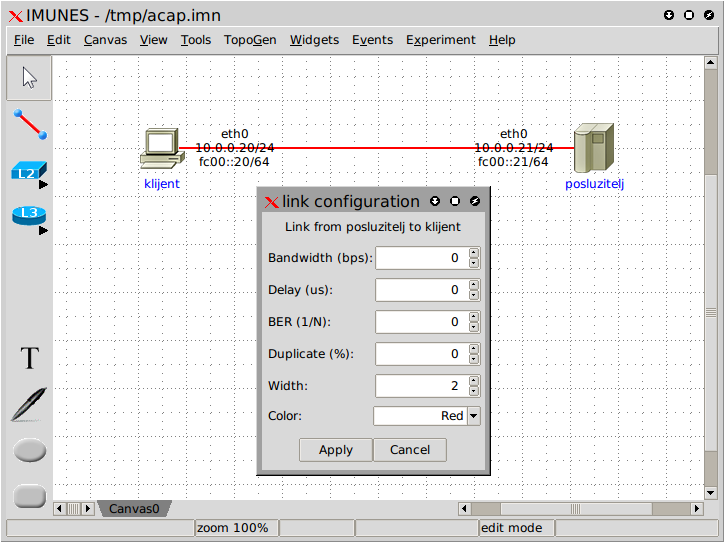
\includegraphics[width=0.82\textwidth]{imunes}
    \caption{Emulirana mrežna topologija za mjerenja u alatu IMUNES}
    \label{fig:imunes}
\end{figure}

Sva opisana mjerenja izvedena su na priloženoj topologiji uz promjenu
parametara na poveznici. Mjerenje kašnjenja izvedeno je u 50 iteracija
te je konačni prosjek prikazan pomoću grafikona i tablica.

\subsection{Utjecaj veličine javnih ključeva na veličinu poruka}

Duljina javnog ključa izravno utječe na veličinu digitalnog potpisa koji se
koristi za zaštitu poruka. S druge strane, duljina ključa povećava razinu
sigurnosti razmjene, ali ujedno i usporava računanje i verifikaciju digitalnih
potpisa. Kako se razvija i napreduje računalna moć tako se javlja potreba za sve
većom razinom sigurnosti. Na slici \ref{fig:key_size} prikazane su veličine
poruka za različite veličine RSA ključeva. Duljine poruka izražene su u
oktetima, dok su duljine ključeva prikazane na standardan način, u bitovima.
Može se zamijetiti kako
poruka \initi{} uopće ne ovisi o veličini javnog ključa jer ne sadrži niti javni
ključ niti digitalni potpis. Poruka \listr{} sadrži samo digitalni potpis, a
poruke \initr{} i \listi{} sadrže i digitalni potpis i javni ključ što je
vidljivo iz slike jer crte koje ih označuju najbrže rastu.

\begin{figure}[h]
    \centering
    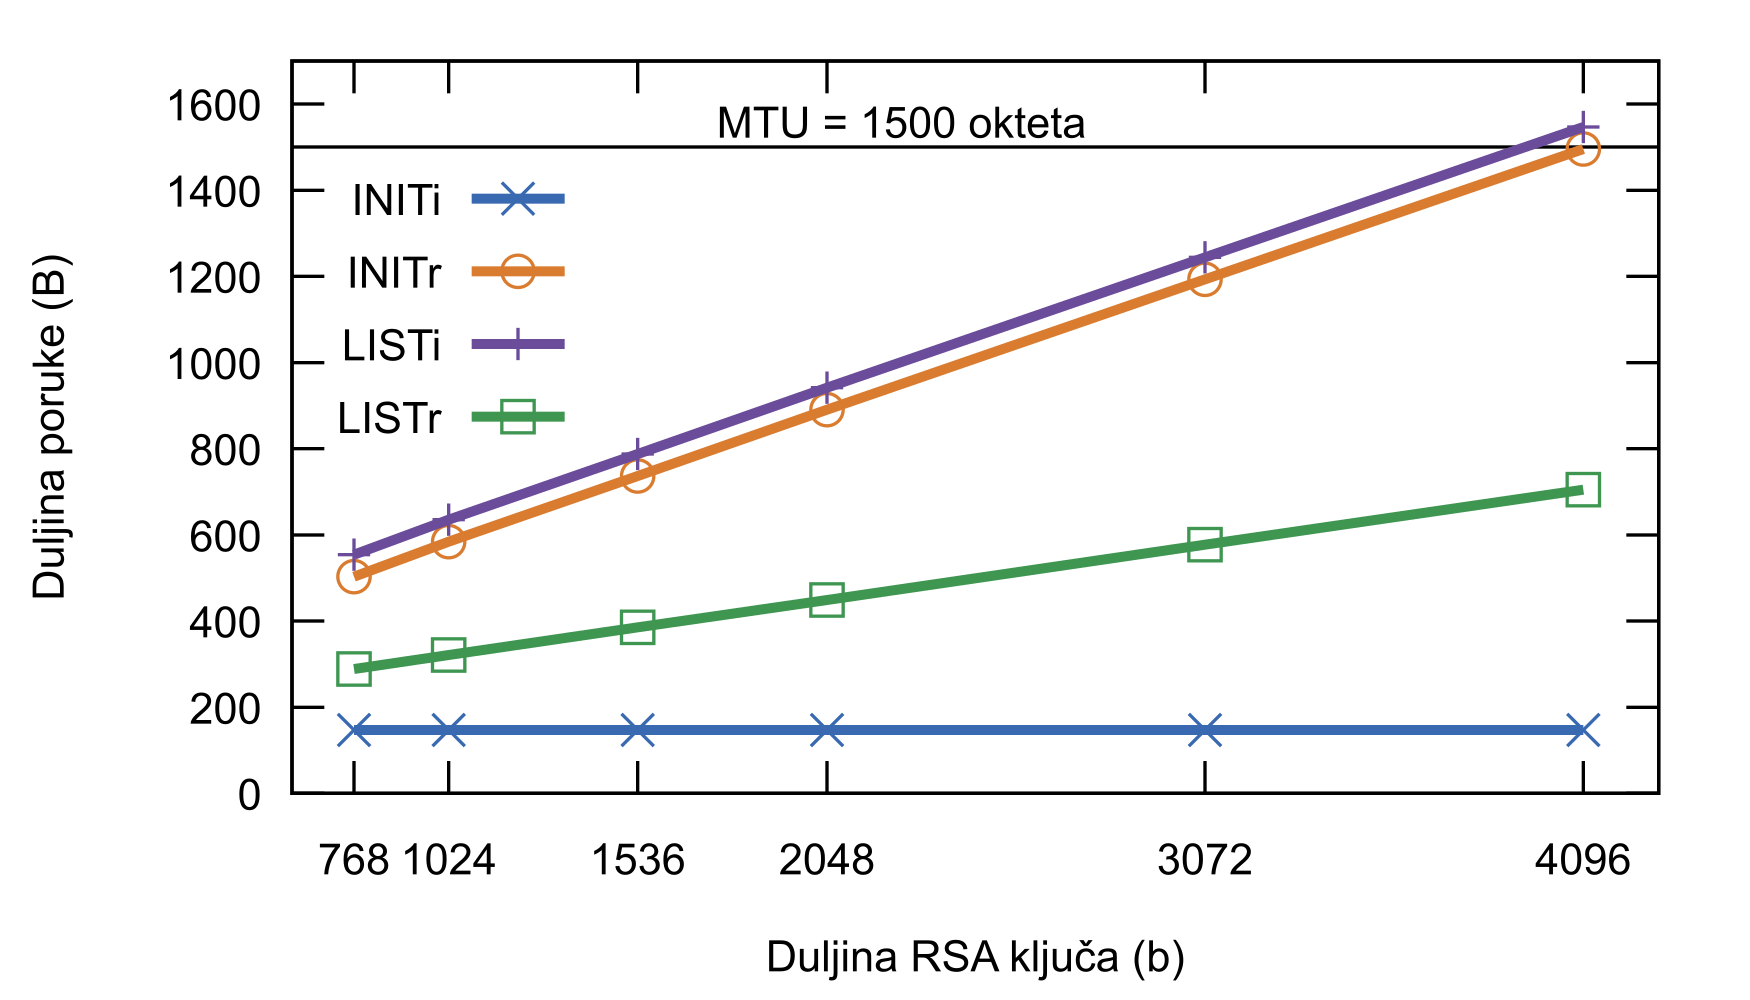
\includegraphics[width=0.7\textwidth]{key_size.png}
    \caption{Veličina poruka ovisno o veličini RSA javnih ključeva}
    \label{fig:key_size}
\end{figure}

Protokol Ethernet standardno podržava prijenos od najviše 1500 okteta podataka,
što je definirano najvećom jedinicom prijenosa (engl. \emph{Maximum
Transmission Unit} - MTU). Povećanje veličine RSA ključeva ili veliki popis podržanih
algoritama mogli bi onemogućiti korištenje protokola na sloju
Ethernet, odnosno zahtijevalo bi se
korištenje više poruka za razmjenu cijelog popisa, što nije predviđeno
specifikacijom i ostvarenjem protokola. Uz to, cilj je smanjiti veličinu
poruka kako bi se
povećala efikasnost i smanjila propusnost potrebna za razmjenu poruka i ubrzao
sam dogovor.

Smanjenje veličine poruka moguće je uvođenjem kriptografije koja se zasniva na
eliptičnim krivuljama i koristi manju veličinu javnih ključeva i digitalnih
potpisa. Mjerenja veličine poruka za različite veličine ECDSA ključeva
prikazana su na slici \ref{fig:key_size_ec}. 

\begin{figure}[h]
    \centering
    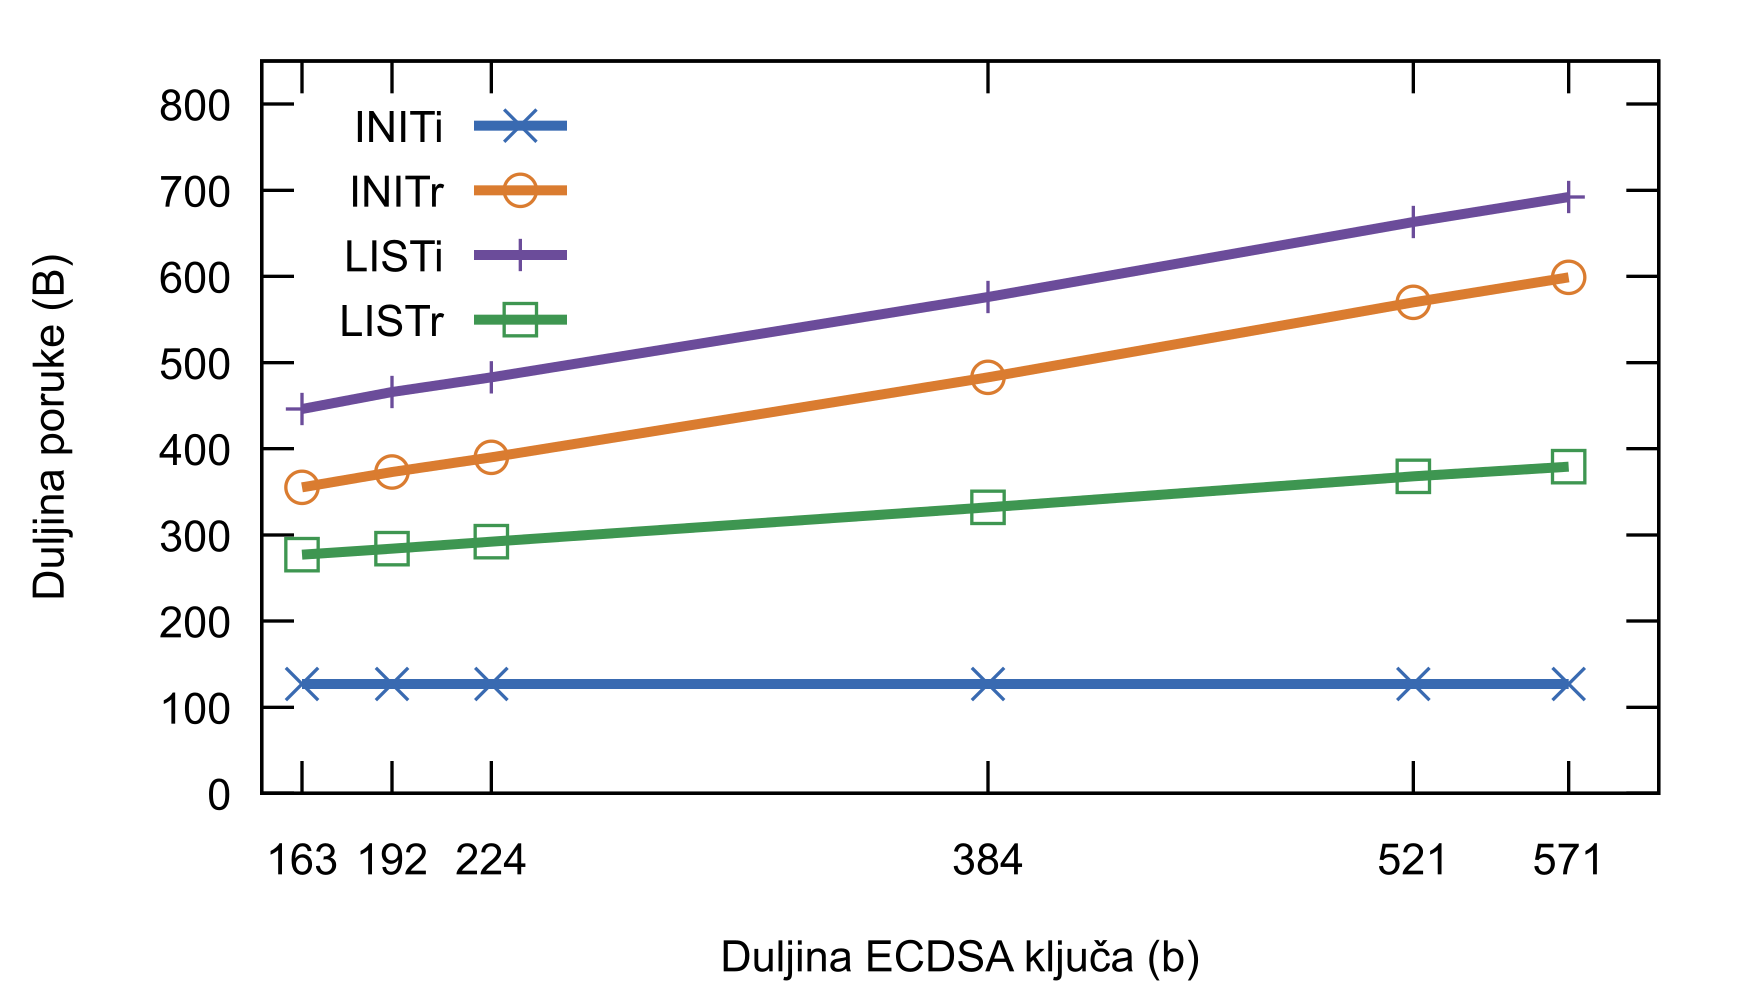
\includegraphics[width=0.7\textwidth]{key_size_ec.png}
    \caption{Veličina poruka ovisno o veličini ECDSA javnih ključeva}
    \label{fig:key_size_ec}
\end{figure}

Korištenjem ECDSA ključeva značajno se smanjuje veličina poruka protokola ACAP i
smanjuje potrebna propusnost za protokol. Važno je napomenuti da je
sigurnost koju pruža 224 bitni ECDSA ključ usporediva sa sigurnošću koju pruža
2048 bitni RSA ključ. Stoga, uvođenje kriptografije zasnovane na eliptičnim
krivuljama smanjuje potrebnu propusnost i ujedno povećava razinu sigurnosti.

\subsection{Trajanje dogovora ovisno o kašnjenju}

Trajanje dogovora mjereno je na strani klijenta tako da se jednosmjerno
kašnjenje mijenjalo od 0 ms sve do 400 ms, što predstavlja maksimalno kašnjenje
u oba smjera od 800 ms. Mjerenja su izvršena za sve transportne protokole, ali
razlike između protokola UDP, IPv4, IPv6 i Ethernet su premale i ne daju nikakav
dodatan uvid u mjerenja. Na slici \ref{fig:agreement_delay} prikazana su
mjerenja kašnjenja za protokole UDP, SCTP i TCP uz korištenje standardne
kriptografije i uz korištenje kriptografije zasnovane na eliptičkim krivuljama.

\begin{figure}[h]
    \centering
    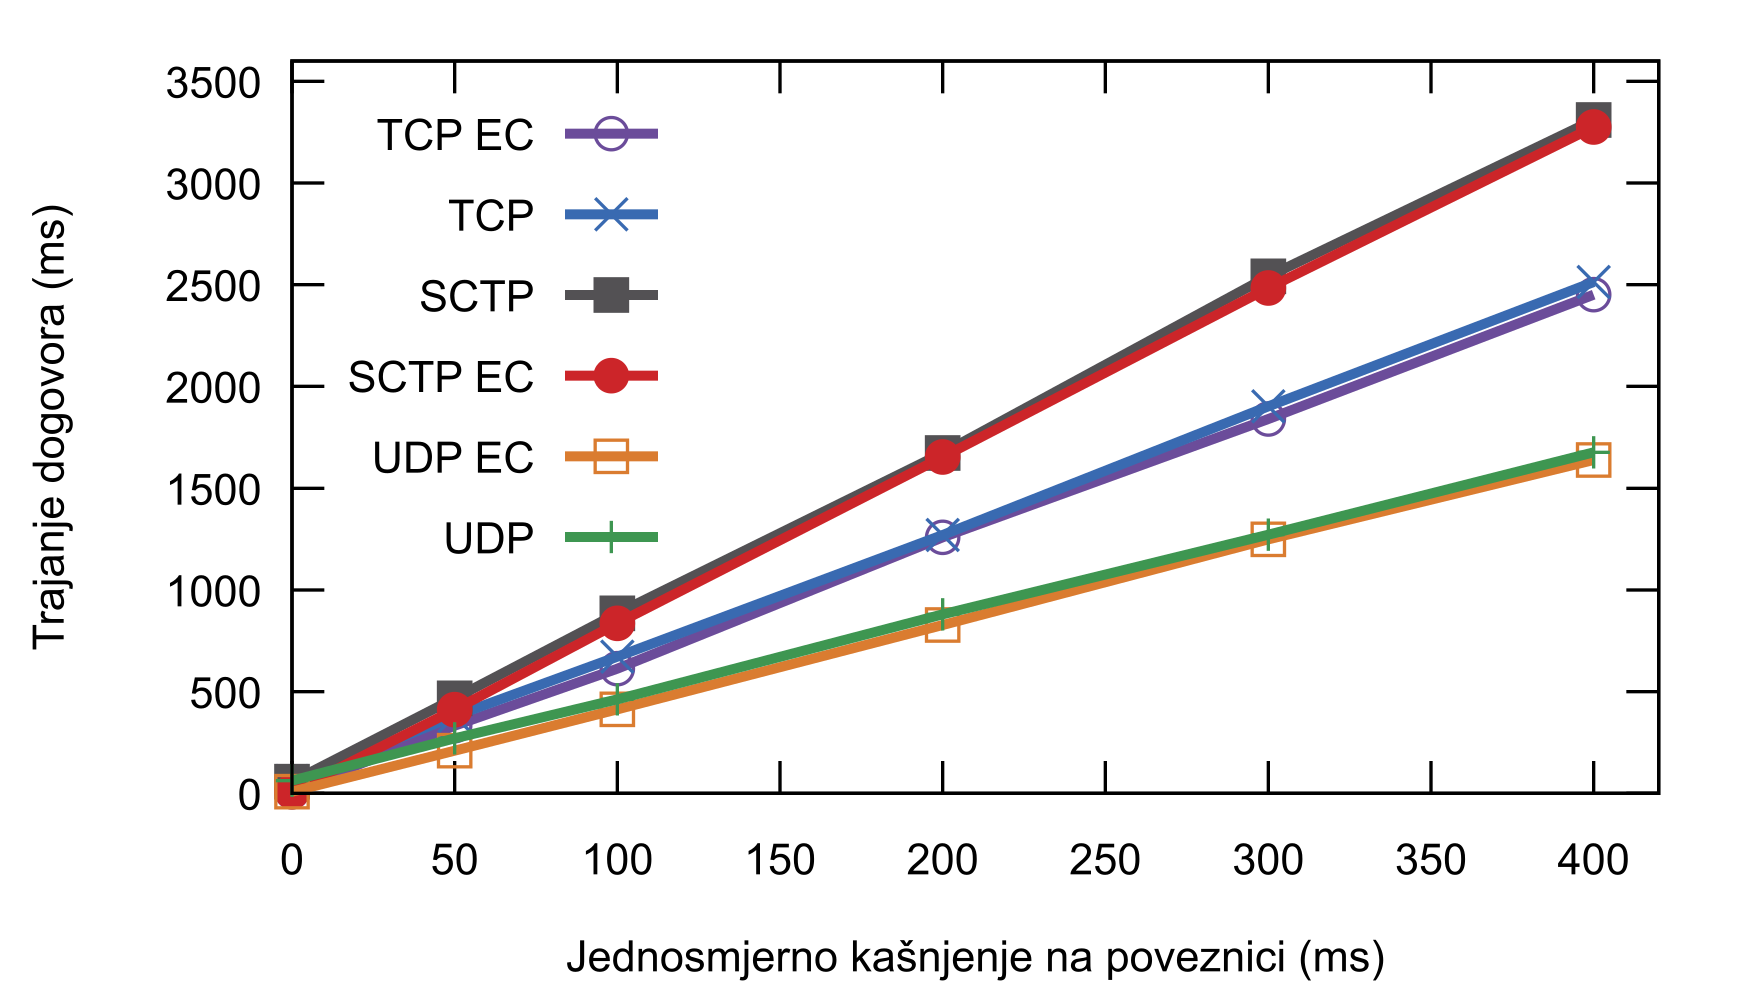
\includegraphics[width=0.7\textwidth]{agreement_delay2.png}
    \caption{Trajanje dogovora ovisno o kašnjenju, protokolu i korištenim algoritmima}
    \label{fig:agreement_delay}
\end{figure}

Prije svega, mogu se zamijetiti razlike između protokola UDP, SCTP i TCP koje su
ovisne o uspostavi veze kod tih protokola. UDP nema nikakve uspostave, protokolu
SCTP su potrebne 4 poruke, a protokolu TCP 3 poruke za uspostavu
veze. Slika \ref{fig:agreement_delay} ujedno pokazuje da je korištenje
eliptičnih krivulja manje zahtjevno, ali da i mala vrijednost kašnjenja
značajnije utječe na trajanje dogovora u odnosu na promjenu kriptografskih
operacija.

\subsection{Utjecaj propusnosti na trajanje dogovora}

Na slici \ref{fig:agreement_bw} prikazano je trajanje dogovora u odnosu na
brzinu u kilobitima u sekundi (Kbps). U mjerenja nisu uključeni rezultati za
više od 10 Mbps jer iznad te brzine nema razlike u trajanju dogovora. Protokol
ACAP ima
relativno male zahtjeve na propusnost jer se dogovor može dovršiti i na
poveznici brzine 10 Kbps ispod 2 sekunde.

\begin{figure}[h]
    \centering
    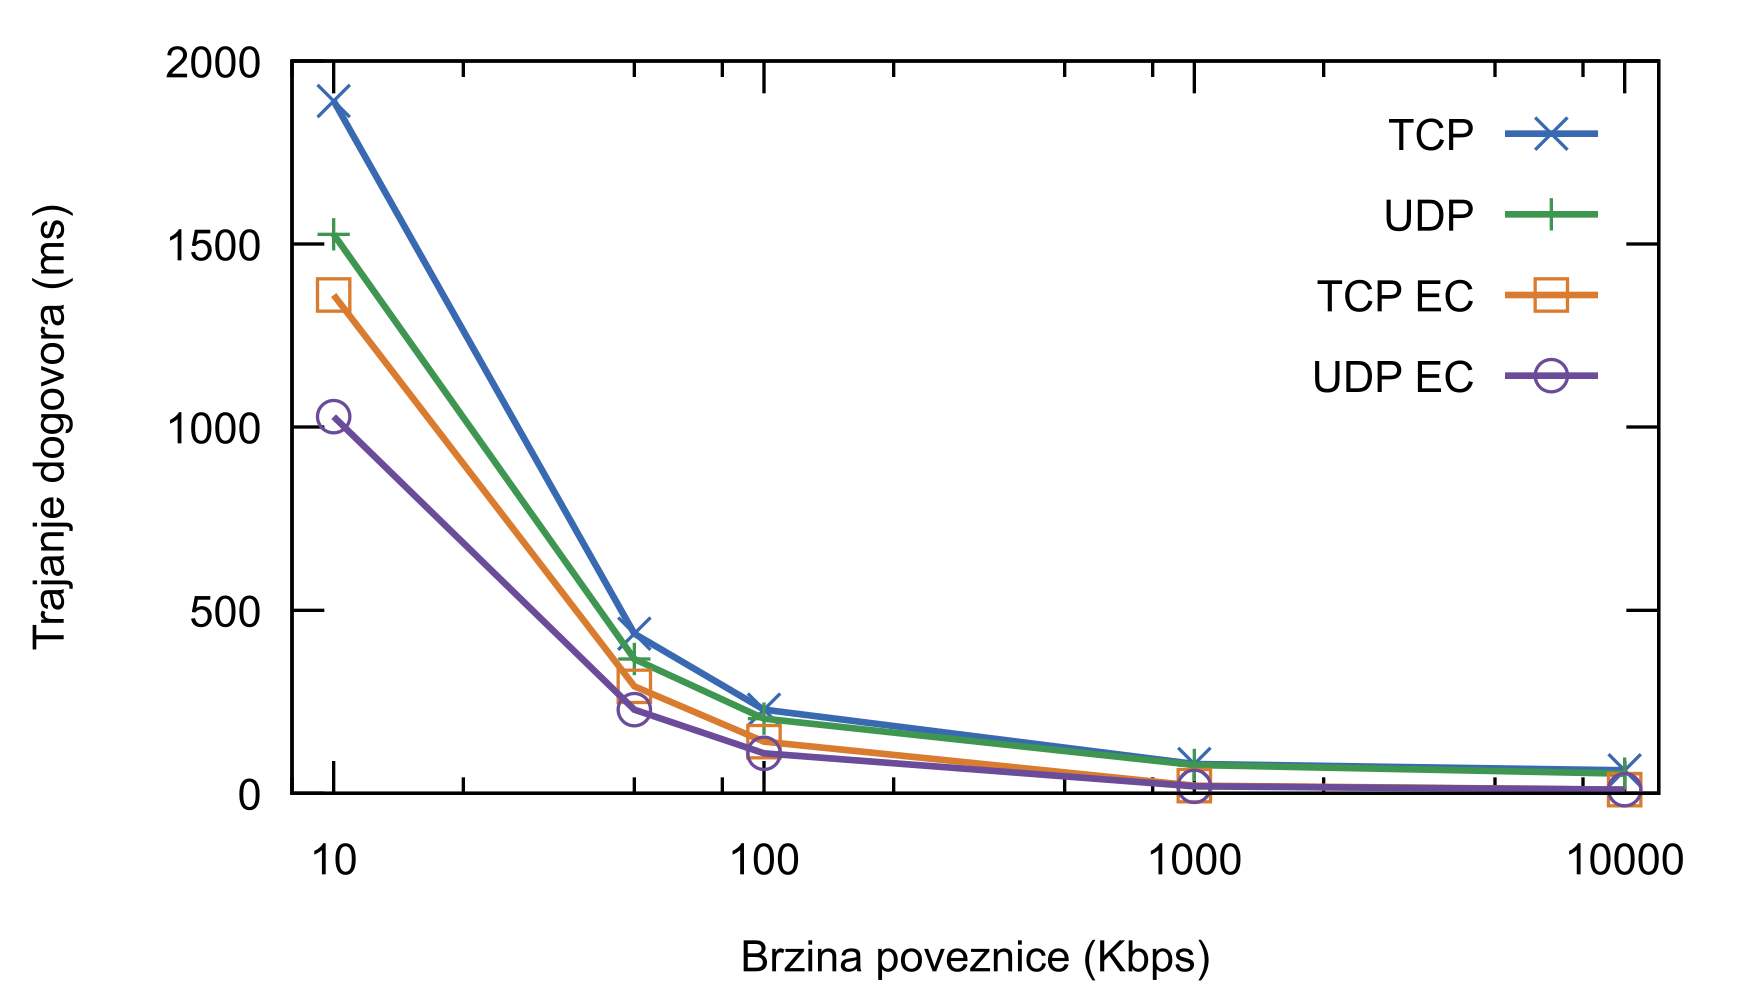
\includegraphics[width=0.7\textwidth]{agreement_bw.png}
    \caption{Trajanje dogovora ovisno o brzini poveznice, protokolu i korištenim algoritmima}
    \label{fig:agreement_bw}
\end{figure}

Uz korištenje kriptografije zasnovane na eliptičnim krivuljama dodatno se
smanjuju zahtjevi na propusnost poveznice, što ih čini osobito pogodnim za
dogovor na uređajima s ograničenim sposobnostima koji su prisutni u okolini
Interneta stvari.

Slika također pokazuje da je dodatan promet koji koriste standardni
kriptografski algoritmi u odnosu na EC algoritme veći od dodatnog prometa koji
generira signalizacija protokola TCP. U slučaju korištenja EC algoritama
dovoljno se ubrzava dogovor korištenjem protokola TCP, koji u tom slučaju postaje
valjana alternativa protokolu UDP i u uvjetima niske propusnosti.

\section{Složenost kriptografskih operacija u protokolu}
\label{sec:complex}

U protokolu ACAP izvode se sljedeće kriptografske operacije:
\begin{itemize}
    \item generiranje tajnog i javnog dijela za Diffie-Hellman razmjenu,
    \item računanje DH zajedničke tajne,
    \item računanje i provjera digitalnog potpisa i
    \item računanje i provjera HMAC zaštitne sume.
\end{itemize}

Trajanje stvaranja i obrade svake poruke u protokolu ACAP prikazano je u
tablici \ref{tab:obrada}. U tablici su vremena za stvaranje poruka označena
žutom bojom, dok su vremena obrade neoznačena. Mjerenja su rađena korištenjem standardnih
Diffie-Hellman parametara veličine 1536 bita te za ECDH korištenjem 163 bitne
eliptične krivulje koji pružaju usporedive razine sigurnosti. Za digitalni
potpis korišten je RSA-1536 kod standardnih algoritama, a ECDSA-sect163r2 kod EC
algoritama.

\begin{table}[htb]
\caption{Trajanje stvaranja i obrade poruka}
\renewcommand{\arraystretch}{1.3}
\label{tab:obrada}
\centering
\normalsize
\begin{tabular}{ l  r  r  r  r }
\toprule &
    Klijent &
    Poslužitelj &
    Klijent EC &
    Poslužitelj EC
    \\ \midrule
\initi{} &
    \colorbox{yellow!50}{47.207 ms} &
    \colorbox{white!50}{4.157 ms} &
    \colorbox{yellow!50}{1.483 ms} &
    \colorbox{white!50}{0.676 ms}
    \\ \hline
\initr{} &
    \colorbox{white!50}{4.284 ms} &
    \colorbox{yellow!50}{0.172 ms} &
    \colorbox{white!50}{1.125 ms} &
    \colorbox{yellow!50}{0.162 ms}
    \\ \hline
\listi{} &
    \colorbox{yellow!50}{0.365 ms} &
    \colorbox{white!50}{0.282 ms} &
    \colorbox{yellow!50}{0.432 ms} &
    \colorbox{white!50}{0.636 ms}
    \\ \hline
\listr{} &
    \colorbox{white!50}{0.171 ms} &
    \colorbox{yellow!50}{0.257 ms} & 
    \colorbox{white!50}{0.599 ms} &
    \colorbox{yellow!50}{0.342 ms}
    \\ \hline
Ukupno &
    52.009 ms &
    4.869 ms &
    3.460 ms &
    1.817 ms
    \\ \bottomrule
\end{tabular}
\end{table}

Za stvaranje poruke \initi{} potrebno je generirati tajni i javni dio za
Diffie-Hellman razmjenu na klijentskoj strani. To je računalno najzahtjevniji
dio cijelog dogovora i za standardne i za EC algoritme, što se odražava u
vremenima u tablici. Obrada poruke \initi{}
na poslužiteljskoj strani sastoji se od računanja Diffie-Hellman zajedničke
tajne, što predstavlja drugu najzahtjevniju operaciju u sklopu razmjene poruka.

Stvaranje poruke \initr{} uključuje izračun digitalnog potpisa i HMAC sažetka.
Izračun digitalnog potpisa kod poslužitelja odrađuje se u sklopu pozadinskog
procesa u svrhu smanjivanja utjecaj DoS napada na protokol ACAP, a izračun
HMAC-a može se odraditi tek po primitku poruke \initi{}. Obrada poruke
\initr{} sastoji se od provjere digitalnog potpisa i HMAC-a te računanja DH
zajedničke tajne. Dok su za standardne algoritme stvaranje i obrada \initr{}
slične zahtjevnosti, kod ECDSA algoritama složenost provjere digitalnog potpisa
veća je od složenosti računanja (za algoritam RSA vrijedi suprotno).

Stvaranje poruke \listi{} obuhvaća računanje digitalnog potpisa i HMAC zaštitne
sume koji se po primitku provjeravaju na strani poslužitelja. Posljednja poruka
\listr{} sadrži samo digitalni potpis koji se provjerava na strani klijenta
nakon primitka poruke. Kod ove poruke uočava se složenost stvaranja i
provjeravanja digitalnog potpisa kod standardnih i EC algoritama.

Ukupni rezultati mjerenja pokazuju kako je opterećenje veće na strani
klijenta u odnosu na poslužitelja, kod standardnih algoritama taj je odnos
veći nego kod EC algoritama zbog računalno zahtjevnog generiranja
dobrih Diffie-Hellman vrijednosti za zaštitu komunikacije. Razlika između
klijenta i poslužitelja postoji jer poslužitelj u pozadini generira DH
vrijednosti. Po potrebi bi se to moglo raditi i na klijentskoj strani kako bi se
smanjilo opterećenje kod početka dogovora.

\section{Dohvaćanje podržanih algoritama}

Dohvaćanje trenutno podržanih algoritama u sustavu izvedeno je pomoću vanjskog
alata koji generira listu u JSON formatu koja je kompatibilna s aktualnim
programskim ostvarenjem protokola ACAP. Rezultat izvođenja prikazan je na slici
\ref{fig:fetch_algs}. U danom primjeru algoritmi su raspoređeni po abecedi,
a konačan raspored uvjetovan je željenom razinom sigurnosti i ostalim
uvjetima okoline u kojoj se protokol izvodi. Primjerice, u uređaje se mogu
ugraditi prioriteti ili se oni mogu dohvaćati s nekog vanjskog servisa koji
će redovito rangirati kriptografske algoritme ovisno o duljini ključa ili izlaza i
postojećim napadima na te algoritme. Na raspoređivanje algoritama mogu
utjecati i različiti dokumenti i specifikacije vezani uz određenu
ustanovu, propisane standarde\footnote{Popis aktualnih standarda i preporuka
može se naći na: \url{http://www.keylength.com/}.} ili postupak certifikacije.

\begin{figure}[htb]
\begin{footnotesize}
\begin{verbatim}
{
  "algorithm types": {
    "hash": [
      "MD5", "RIPEMD160", "SHA1", "SHA224", "SHA256", "SHA384", "SHA512", "Whirlpool" ],
    "public_key": [
      "DSA_1024", "DSA_2048", "DSA_3072", "RSA_1024", "RSA_1536", "RSA_2048",
      "RSA_3072", "RSA_4096", "ECDSA_prime256v1_256", "ECDSA_sect163k1_163",
      "ECDSA_secp384r1_384", ... ],
    "secret_key": [
      "AES_ECB_128", "AES_CBC_128", "AES_CTR_128", "AES_ECB_192", "AES_CBC_192",
      "AES_CTR_192", "AES_ECB_256", "AES_CBC_256", "AES_CTR_256", "Blowfish_ECB_128",
      "Blowfish_CBC_128", ...  "Blowfish_CBC_152", "Blowfish_CTR_152", "CAST5_ECB_64",
      "CAST5_CBC_80", ...  "CAST5_ECB_112", "CAST5_CBC_112", "CAST5_CTR_112",
      "Camellia_ECB_128", "Camellia_CBC_128", ...  "Camellia_ECB_256", "Camellia_CBC_256",
      "Camellia_CTR_256", "IDEA_ECB_128", "IDEA_CBC_128", "IDEA_CTR_128", "SEED_ECB_128",
      "SEED_CBC_128", "SEED_CTR_128", "TripleDES_ECB_64", "TripleDES_CBC_64",
      "TripleDES_CTR_64", "TripleDES_ECB_128", "TripleDES_CBC_128", "TripleDES_CTR_128",
      "TripleDES_ECB_192", "TripleDES_CBC_192", "TripleDES_CTR_192" ]
  }
}
\end{verbatim}
\end{footnotesize}
\vspace{-20pt}
\caption{Skraćeni ispis alata za dohvaćanje podržanih kriptografskih algoritama}
\label{fig:fetch_algs}
\end{figure}

Trenutno podržani algoritmi ovise isključivo o biblioteci koja će se koristiti
za zaštitu komunikacije nakon dogovora algoritma, odnosno o vanjskoj aplikaciji
koja koristi protokol ACAP za dogovor svih preduvjeta potrebnih za zaštitu
komunikacije. U danom primjeru dohvaćaju se podržani algoritmi koje koristi
biblioteka \emph{cryptography} za Python 3 koja se radi brzine izvođenja oslanja
na biblioteku OpenSSL\footnote{https://www.openssl.org/}.

\section{Ostvareni sigurnosni mehanizmi}

Sigurnosni mehanizmi u protokolu ACAP uvedeni su na više različitih razina.
Osnovni mehanizmi izravno su vezani uz komunikacijski model te su opisani i
formalno verificirani kroz alat Scyther u poglavlju \ref{ch:verif}.
Ostatak sigurnosnih mehanizama izravno je vezan uz ostvarenje prototipa.
Ostvareni su sljedeći sigurnosni mehanizmi:
\begin{itemize}
    \item smanjenje utjecaja DoS napada iscrpljivanjem resursa na strani
	poslužitelja,
    \item sprječavanje napada ponavljanjem poruka,
    \item neovisnost kriptografskih ključeva za dogovor i ključeva za zaštitu
	komunikacije nakon dogovora.
\end{itemize}

Iz poglavlja \ref{sec:complex} vidljivo je da su najzahtjevnije operacije
vezane uz generiranje Diffie-Hellman vrijednosti i računanje DH tajnog ključa.
Na poslužiteljskoj strani bi se obje te operacije trebale odraditi po primitku
poruke \initi{}. Na taj način bi programsko ostvarenje bilo izravno izloženo
napadu gdje se generira veliki broj \initi{} poruka. Kako bi se spriječio taj
napad, generiranje DH vrijednosti odvojeno je u zasebnu proceduru koja
periodički u pozadini generira DH vrijednosti. Dodatno se uz generiranje vrijednosti
generira i digitalni potpis koji je sastavni dio poruke \initr{} ($S_R(g^r)$)
kako bi se smanjilo opterećenje stvaranja poruke \initr{}. U zadnjem redu
tablice \ref{tab:obrada} prikazane su ukupne vrijednosti obrade za klijenta i
poslužitelja. Te vrijednosti pokazuju da je trošak na strani mogućeg napadača,
odnosno klijenta, veći od troška na strani poslužitelja.

Napadač koji se nalazi na putu između poslužitelja i klijenta mogao bi spremiti
sve pakete uključene tijekom jedne razmjene i kasnije ponoviti cjelokupnu
razmjenu tako da se opet koriste prije dogovoreni ključevi i algoritmi.
Prvi dio obrane od takvog napada leži u osvježavanju DH vrijednosti na strani
poslužitelja, koja se generira svakih 30 sekundi. Novi javni dio DH razmjene
izravno će utjecati na ostatak razmjene te će provjere HMAC sažetka biti
neuspješne. Drugi dio obrane nalazi se u pamćenju prijašnjih \emph{nonce}
vrijednosti i odbijanju paketa s prethodno korištenim \emph{nonce}
vrijednostima.

Neovisnost kriptografskih ključeva postiže se uvođenjem pseudo nasumičnih
funkcija (engl. \emph{pseudo random function}, PRF) koje će iterativnim
korištenjem algoritma HMAC jamčiti računalnu neovisnost ključeva. Koncepti za
ostvarenje PRF-a preuzeti su iz protokola IKEv2~\cite{rfc5996} i jamče da
ključ koji se koristi za dogovor u protokolu ACAP neće otkriti nikakve podatke o
dijeljenom tajnom ključu koji je rezultat protokola ACAP.

% vim: spell spelllang=hr

\chapter{Zaključak}

U doktorskoj disertaciji dizajniran je i programski ostvaren protokol za
sigurno dogovaranje kriptografskih algoritama i ključeva, koji omogućuje
kriptografski prilagodljivu komunikaciju između dva komunicirajuća uređaja.
Kriptografski prilagodljiva komunikacija ključna je u ostvarivanju dugoročno
sigurne komunikacije, što je prikazano u pregledu područja istraživanja.
Model protokola formalno je
specificiran i verificiran u alatu za automatsku provjeru sigurnosti
u odnosu na prethodno postavljene uvjete sigurne komunikacije. Primjena
formalne verifikacije omogućila je dizajn protokola koji zadovoljava sve željene
uvjete sigurne komunikacije.

Dogovor algoritama i ključeva u protokolu ACAP može se izvoditi na način koji je
neovisan o sloju, aplikaciji i trenutnom operacijskom sustavu. 
Analizirana
je integracija protokola u sustav za sigurnu komunikaciju u okolini Interneta
stvari s osvrtom na prilagodljivost odabira algoritma koji uzima u obzir
trenutne
mogućnosti uređaja. Arhitektura protokola omogućuje učinkovit dogovor preduvjeta
sigurne komunikacije u modelu klijent poslužitelj i mrežama ravnopravnih čvorova
s niskim zahtjevima na mrežnu propusnost i računalnu snagu komunicirajućih
strana. Programsko ostvarenje protokola omogućuje korištenje protokola na svim
razinama protokolnog složaja TCP/IP te pokazuje robusnost rješenja i
ostvarene sigurnosne mehanizme.

% vim: spell spelllang=hr


%%%%%%%%%%%%%%%%%%%%%%%%%%%%%%%%%%%%%%%%%%%%%%%%%%%%%%%%%%%%%%%%%%%%%%%%%%%
\backmatter
\chapter{Dodaci}

\addtocontents{toc}{\protect\setcounter{tocdepth}{1}}

\begin{subappendices}
\renewcommand{\thesection}{\Alph{section}}

\section{Potpuni model protokola ACAP} \label{app:model}

\begin{small}
\begin{verbatim}
hashfunction KDF, MAC, g, h;
const incr: Function;
usertype AlgList;

protocol @executability (DH, O) {
  role DH {
    var i, r: Nonce;
    recv_!DH1( DH, DH, h(g(r),i) );
    send_!DH2( DH, DH, h(g(i),r) );
  }
  role O {
    var i, r, Ni, Nr: Nonce;
    var I, R: Agent;
    var Li: AlgList;

    #send_!2( R, I, g(r), Nr, R, {h(g(r))}sk(R), MAC(h(  Gi,r), R, Ni, Nr) );
    recv_!01( O, O, g(r), Nr, R, {h(g(r))}sk(R), MAC(h(g(i),r), R, Ni, Nr) );
    send_!02( O, O, g(r), Nr, R, {h(g(r))}sk(R), MAC(h(g(r),i), R, Ni, Nr) );
    #recv_!2( R, I,   Gr, Nr, R, {h(  Gr)}sk(R), MAC(h(  Gr,i), R, Ni, Nr) );

    #send_!3( I, R, I, Li, {h(Li, g(i),   Gr)}sk(I), MAC(h(  Gr,i), I) );
    recv_!03( O, O, I, Li, {h(Li, g(i), g(r))}sk(I), MAC(h(g(r),i), I) );
    send_!04( O, O, I, Li, {h(Li, g(i), g(r))}sk(I), MAC(h(g(i),r), I) );
    #recv_!3( I, R, I, Li, {h(Li,   Gi, g(r))}sk(I), MAC(h(  Gi,r), I) );
  }
}



protocol acap(I, R) {
  role I {
    fresh i, Ni: Nonce;
    var Nr: Nonce;
    var Gr: Ticket;
    fresh Li: AlgList;
    var Lr: AlgList;
    
    send_1( I, R, g(i), Ni);
    recv_!2( R, I,   Gr, Nr, R, {h(Gr)}sk(R), MAC(h(  Gr,i), R, Ni, Nr) );
    claim_I1( I, Running, R, g(i), Gr);
    send_!3( I, R, I, Li, {h(Li, g(i), Gr)}sk(I), MAC(h(Gr,i), I) );
    recv_4( R, I, Lr, {h(g(i), Gr, Lr)}sk(R) );
    
    claim_I2( I, SKR, KDF(h(Gr,i)) );
    claim_I5( I, Commit, R, g(i), Gr);
    claim_I8( I, Nisynch );
  }
  role R {
    fresh r, Nr: Nonce;
    var Ni: Nonce;
    var Gi: Ticket;
    
    fresh Lr: AlgList;
    var Li: AlgList;
    recv_1( I, R, Gi, Ni);
    claim_R1( R, Running, I, g(r), Gi);
    send_!2( R, I, g(r), Nr, R, {h(g(r))}sk(R), MAC(h(Gi,r), R, Ni, Nr) );
    recv_!3( I, R, I, Li, {h(Li,   Gi, g(r))}sk(I), MAC(h(  Gi,r), I) );
    send_4( R, I, Lr, {h(Gi, g(r), Lr)}sk(R) );
    
    claim_R2( R, SKR, KDF(h(Gi,r)) );
    claim_R5( R, Commit, I, g(r), Gi);
    claim_R8( R, Nisynch );
  }
}
\end{verbatim}
\end{small}

\section{Ispis izvođenja programskog ostvarenja} \label{app:impl}

\subsection{Klijentska strana} \label{app:cli_impl}

\begin{small}
\begin{verbatim}
$ ./acap.py -C -a client.json -k private_key_client -l 10 -h 127.0.0.1
DEBUG - CREATE duration: 98489
DEBUG - Client created
DEBUG - host: ('127.0.0.1', 13000)
DEBUG - Client setup
DEBUG - Client connect
DEBUG - Client dh: 68:1c:97:72:1f:ca:8a:7c:5b:15:c3:a6:6a:88:67:37:99:b5:2c:67
:67:23:ae:e0:52:94:fd:a0:99:f7:d7:85:2d:2a:52:94:b4:f4:fc:2e:c8:d2:20:ec:9b:0a
:56:da:8a:7e:36:87:ce:5e:6e:ac:42:50:ee:ad:73:cc:6a:d5:8c:fb:b5:3d:53:bb:32:21
:3b:57:80:df:34:69:6d:67:62:42:93:7f:09:fb:b7:3c:48:4a:8e:d6:ae:bf:78:b6:ca:2b
:d5:7c:4c:ab:ee:64:e0:99:25:bf:17:10:0b:61:ec:cb:b8:5b:a7:d7:02:b0:ea:1e:03:8a
:cd:a4:4a:cf
DEBUG - Client Nonce: 23:16:66:f8:a4:85:18:16:64:0c:b6:06
INFO - Client public key:
-----BEGIN PUBLIC KEY-----
MIGfMA0GCSqGSIb3DQEBAQUAA4GNADCBiQKBgQC4TDSclGnCkXgP0C8mt889rBRl
iFoXBtOlG4VF1XxhxursgU+Es2PCqRUYT28ZqdNrq2CAyuIT33G5CXCwg8x/CBh2
qmFJ43NpauGg13b2LFNSg3j8UxxwGSGIvKvxOmaGnSJByepogXkWuY0bL5mR0n0l
JPH/imO5V2+Jox951QIDAQAB
-----END PUBLIC KEY-----
DEBUG - PREP_INIT_I duration: 79
DEBUG - PROC_INIT_R duration: 6586
DEBUG - Server dh: 94:44:cc:29:f1:dc:14:66:d8:ce:07:90:ca:5d:77:64:0b:7c:21:16
:ef:42:31:a4:bf:50:cd:94:8b:71:1b:29:30:1d:20:f0:0e:6e:d6:56:8e:b4:9c:cd:58:5f
:54:12:a1:04:eb:32:43:6d:e7:5a:d0:6d:23:0b:6b:2f:7e:5a:0d:40:fb:4c:c7:bd:ee:b7
:0a:e3:ba:df:06:11:49:78:77:6b:fc:37:f5:f2:c3:84:18:44:e3:9a:28:42:0d:76:ea:59
:27:71:41:24:07:07:3d:88:40:eb:c9:67:25:bc:ea:4c:72:c7:98:9d:7d:dd:11:25:50:b5
:2d:b3:84:79
DEBUG - DH key: f7:d8:2a:83:a2:58:55:e4:af:02:aa:da:d2:f2:c7:f2:75:62:a7:95:cb
:e7:b7:50:ee:f7:6d:cd:4b:35:98:ee:38:d4:53:bc:b8:91:ba:a4:82:88:cc:18:2d:55:fd
:79:ab:3d:48:16:17:84:78:bb:45:cb:60:a9:05:ee:78:78:e4:bc:7c:75:cc:b0:c0:a2:7e
:69:53:fa:e4:1f:d2:d0:26:75:61:97:94:33:7c:6e:3e:88:44:61:92:10:ee:92:bc:71:ab
:e4:84:ae:68:0b:fc:aa:db:3b:73:9d:e8:94:86:0e:ef:fe:10:33:12:0e:6d:a5:59:ac:78
:a6:bd:a9
DEBUG - Server Nonce: df:69:de:1a:d8:13:c7:b0:74:0a:71:7a
INFO - Server public key:
-----BEGIN PUBLIC KEY-----
MIGfMA0GCSqGSIb3DQEBAQUAA4GNADCBiQKBgQCTYB3xU17CS5AGxKbWraxuGOYb
7sff8AAjjiwXrdBr6jqJ5zSHtR/bKxsRNPMNvzihVI1Taa7/CQy3EIRKkLeG4I7M
USeStpBfvQlpAK+lmyUE3haXVUNgPpALdXUpn+IaB+TDHuWl19z9dPDkSDLzQzga
pVwSgXpEZDUInwKK4QIDAQAB
-----END PUBLIC KEY-----
DEBUG - Client LIST: {"algorithm types": {"hash": ["SHA-256", "RIPEMD",
 "SHA-1"], "public_key": ["RSA_1024", "RSA_2048", "ECDSA_192"], "secret_key":
 ["AES-CTR_256", "3DES_192", "AES-CBC_128"]}}
DEBUG - PREP_LIST_I duration: 621
DEBUG - PROC_LIST_R duration: 259
DEBUG - Server LIST: {"algorithm types": {"hash": ["SHA3-512", "SHA-512",
 "SHA-256"], "public_key": ["ECDSA_192", "ECDSA_224", "RSA_2048"], "secret_key":
 ["AES-CTR_256", "Salsa20_256", "AES-CBC_128"]}}
DEBUG - NEGOTIATE duration: 104
INFO - Client negotiated: 
{
    "hash": {
        "algorithm": "SHA-256",
        "timestamp": "2015-11-22 14:59"
    },
    "public_key": {
        "algorithm": "RSA_2048",
        "timestamp": "2015-11-22 14:59"
    },
    "secret_key": {
        "algorithm": "AES-CTR_256",
        "timestamp": "2015-11-22 14:59"
    }
}
INFO - Shared secret key (256 bit): bb:66:cc:98:10:fd:b7:a0:73:9b:9e:35:49:11:
43:7e:e5:28:3d:b3:69:5e:e2:69:4c:c9:a8:11:6d:d5:57:9a
INFO - TOTAL duration: 119820
\end{verbatim}
\end{small}

\subsection{Poslužiteljska strana} \label{app:serv_impl}

\begin{small}
\begin{verbatim}
$ ./acap.py -S -a server.json -k private_key_server -l 10
DEBUG - CREATE duration: 1897
Refreshed DH and Nonce...
DEBUG - Server created
DEBUG - Server listening
DEBUG - Server accepted
DEBUG - Server dh: 94:44:cc:29:f1:dc:14:66:d8:ce:07:90:ca:5d:77:64:0b:7c:21:16
:ef:42:31:a4:bf:50:cd:94:8b:71:1b:29:30:1d:20:f0:0e:6e:d6:56:8e:b4:9c:cd:58:5f
:54:12:a1:04:eb:32:43:6d:e7:5a:d0:6d:23:0b:6b:2f:7e:5a:0d:40:fb:4c:c7:bd:ee:b7
:0a:e3:ba:df:06:11:49:78:77:6b:fc:37:f5:f2:c3:84:18:44:e3:9a:28:42:0d:76:ea:59
:27:71:41:24:07:07:3d:88:40:eb:c9:67:25:bc:ea:4c:72:c7:98:9d:7d:dd:11:25:50:b5
:2d:b3:84:79
DEBUG - Server Nonce: df:69:de:1a:d8:13:c7:b0:74:0a:71:7a
INFO - Server public key:
-----BEGIN PUBLIC KEY-----
MIGfMA0GCSqGSIb3DQEBAQUAA4GNADCBiQKBgQCTYB3xU17CS5AGxKbWraxuGOYb
7sff8AAjjiwXrdBr6jqJ5zSHtR/bKxsRNPMNvzihVI1Taa7/CQy3EIRKkLeG4I7M
USeStpBfvQlpAK+lmyUE3haXVUNgPpALdXUpn+IaB+TDHuWl19z9dPDkSDLzQzga
pVwSgXpEZDUInwKK4QIDAQAB
-----END PUBLIC KEY-----
DEBUG - RECV duration: 1863387
DEBUG - PROC_INIT_I duration: 5955
DEBUG - Client dh: 68:1c:97:72:1f:ca:8a:7c:5b:15:c3:a6:6a:88:67:37:99:b5:2c:67
:67:23:ae:e0:52:94:fd:a0:99:f7:d7:85:2d:2a:52:94:b4:f4:fc:2e:c8:d2:20:ec:9b:0a
:56:da:8a:7e:36:87:ce:5e:6e:ac:42:50:ee:ad:73:cc:6a:d5:8c:fb:b5:3d:53:bb:32:21
:3b:57:80:df:34:69:6d:67:62:42:93:7f:09:fb:b7:3c:48:4a:8e:d6:ae:bf:78:b6:ca:2b
:d5:7c:4c:ab:ee:64:e0:99:25:bf:17:10:0b:61:ec:cb:b8:5b:a7:d7:02:b0:ea:1e:03:8a
:cd:a4:4a:cf
DEBUG - Client Nonce: 23:16:66:f8:a4:85:18:16:64:0c:b6:06
DEBUG - DH key: f7:d8:2a:83:a2:58:55:e4:af:02:aa:da:d2:f2:c7:f2:75:62:a7:95:cb
:e7:b7:50:ee:f7:6d:cd:4b:35:98:ee:38:d4:53:bc:b8:91:ba:a4:82:88:cc:18:2d:55:fd
:79:ab:3d:48:16:17:84:78:bb:45:cb:60:a9:05:ee:78:78:e4:bc:7c:75:cc:b0:c0:a2:7e
:69:53:fa:e4:1f:d2:d0:26:75:61:97:94:33:7c:6e:3e:88:44:61:92:10:ee:92:bc:71:ab
:e4:84:ae:68:0b:fc:aa:db:3b:73:9d:e8:94:86:0e:ef:fe:10:33:12:0e:6d:a5:59:ac:78
:a6:bd:a9
DEBUG - PREP_INIT_R duration: 295
DEBUG - SEND duration: 31
DEBUG - RECV duration: 8441
DEBUG - PROC_LIST_I duration: 492
INFO - Client public key:
-----BEGIN PUBLIC KEY-----
MIGfMA0GCSqGSIb3DQEBAQUAA4GNADCBiQKBgQC4TDSclGnCkXgP0C8mt889rBRl
iFoXBtOlG4VF1XxhxursgU+Es2PCqRUYT28ZqdNrq2CAyuIT33G5CXCwg8x/CBh2
qmFJ43NpauGg13b2LFNSg3j8UxxwGSGIvKvxOmaGnSJByepogXkWuY0bL5mR0n0l
JPH/imO5V2+Jox951QIDAQAB
-----END PUBLIC KEY-----
DEBUG - Client LIST: {"algorithm types": {"hash": ["SHA-256", "RIPEMD",
 "SHA-1"], "public_key": ["RSA_1024", "RSA_2048", "ECDSA_192"], "secret_key":
 ["AES-CTR_256", "3DES_192", "AES-CBC_128"]}}
DEBUG - Server LIST: {"algorithm types": {"hash": ["SHA3-512", "SHA-512",
 "SHA-256"], "public_key": ["ECDSA_192", "ECDSA_224", "RSA_2048"], "secret_key":
 ["AES-CTR_256", "Salsa20_256", "AES-CBC_128"]}}
DEBUG - PREP_LIST_R duration: 357
DEBUG - SEND duration: 28
DEBUG - NEGOTIATE duration: 75
INFO - Server negotiated: 
{   
    "hash": {
        "algorithm": "SHA-256",
        "timestamp": "2015-11-22 14:59"
    },
    "public_key": {
        "algorithm": "RSA_2048",
        "timestamp": "2015-11-22 14:59"
    },
    "secret_key": {
        "algorithm": "AES-CTR_256",
        "timestamp": "2015-11-22 14:59"
    }
}
INFO - Shared secret key (256 bit): bb:66:cc:98:10:fd:b7:a0:73:9b:9e:35:49:11
:43:7e:e5:28:3d:b3:69:5e:e2:69:4c:c9:a8:11:6d:d5:57:9a
INFO - TOTAL duration: 17757
\end{verbatim}
\end{small}

\section{Formati poruka} \label{app:formats}

\subsection{Format poruke \initi{}}
    \centering
\begin{bytefield}[bitwidth=0.80em]{32}
    \bitheader{0,7,15,23,31} \\
    \bitbox{16}{Duljina poruke} &
    \bitbox{8}{Tip=0} &
    \bitbox{8}{Duljina DH} \\
    \bitbox{8}{Duljina DH} & \bitbox[lr]{24}{} \\
    \wordbox[lr]{2}{Klijentov Diffie-Hellman javni dio \\ $\vdots$} \\
    \bitbox{16}{Duljina \emph{noncea}} &
    \bitbox[lrt]{16}{} \\
    \wordbox[lrb]{2}{Klijentov \emph{nonce} \\
    $\vdots$}
\end{bytefield}
\flushleft

\subsection{Format poruke \initr{}}
    \centering
\begin{bytefield}[bitwidth=0.80em]{32}
\bitheader{0,7,15,23,31} \\
\bitbox{16}{Duljina poruke} & \bitbox{8}{Tip=1} & \bitbox{8}{Duljina DH} \\
\bitbox{8}{Duljina DH} & \bitbox[lr]{24}{} \\
\wordbox[lr]{2}{Poslužiteljev Diffie-Hellman javni dio \\ $\vdots$} \\
\bitbox{16}{Duljina \emph{noncea}} & \bitbox[lrt]{16}{} \\
\wordbox[lr]{2}{Poslužiteljev \emph{nonce} \\ $\vdots$} \\
\bitbox{16}{Duljina ključa} & \bitbox[lrt]{16}{} \\
\wordbox[lr]{2}{Javni ključ poslužitelja \\ $\vdots$} \\
\bitbox{16}{Duljina potpisa} & \bitbox[lrt]{16}{} \\
\wordbox[lr]{2}{Digitalni potpis \\ $\vdots$} \\
\bitbox{16}{Duljina HMAC-a} & \bitbox[lrt]{16}{} \\
\wordbox[lrb]{2}{HMAC \\ $\vdots$}
\end{bytefield}
\flushleft

\subsection{Format poruke \listi{}}
    \centering
\begin{bytefield}[bitwidth=0.80em]{32}
\bitheader{0,7,15,23,31} \\
\bitbox{16}{Duljina poruke} & \bitbox{8}{Tip=2} & \bitbox{8}{Duljina ključa} \\
\bitbox{8}{Duljina ključa} & \bitbox[lrt]{24}{} \\
\wordbox[lr]{2}{Javni ključ poslužitelja \\ $\vdots$} \\
\bitbox{16}{Duljina popisa} & \bitbox[lrt]{16}{} \\
\wordbox[lr]{2}{Popis algoritama klijenta \\ $\vdots$} \\
\bitbox{16}{Duljina potpisa} & \bitbox[lrt]{16}{} \\
\wordbox[lr]{2}{Digitalni potpis \\ $\vdots$} \\
\bitbox{16}{Duljina HMAC-a} & \bitbox[lrt]{16}{} \\
\wordbox[lrb]{2}{HMAC \\ $\vdots$}
\end{bytefield}
\flushleft

\subsection{Format poruke \listr{}}
    \centering
\begin{bytefield}[bitwidth=0.80em]{32}
\bitheader{0,7,15,23,31} \\
\bitbox{16}{Duljina poruke} & \bitbox{8}{Tip=3} & \bitbox{8}{Duljina popisa} \\
\bitbox{8}{Duljina popisa} & \bitbox[lrt]{24}{} \\
\wordbox[lr]{2}{Popis algoritama poslužitelja \\ $\vdots$} \\
\bitbox{16}{Duljina potpisa} & \bitbox[lrt]{16}{} \\
\wordbox[lrb]{2}{Digitalni potpis \\ $\vdots$} \\
\end{bytefield}

\end{subappendices}


%%%%%%%%%%%%%%%%%%%%%%% LITERATURA / BIBLIOGRAPHY %%%%%%%%%%%%%%%%%%%%%%%%%
% bibliography style file is modified IEEEtran.bst file,
% changed to suit FER's literature style
\addcontentsline{toc}{chapter}{Literatura}
\bibliographystyle{bib/IEEEtranFER} 
\bibliography{bib/anap,bib/rfc,bib/iot}

%%%%%%%%%%%%%%%%%%%%%%% POPIS OZNAKA / NOMENCLATURE %%%%%%%%%%%%%%%%%%%%%%%
% notation and list of symbols if needed
\printnomenclature

%%%%%%%%%%%%%%%%%%%%%%%%%%% KAZALO POJMOVA / INDEX %%%%%%%%%%%%%%%%%%%%%%%%
% optional index
%\printindex

%%%%%%%%%%%%%%%%%%%%%%%%%%%%%%%%% LOF %%%%%%%%%%%%%%%%%%%%%%%%%%%%%%%%%%%%%
% insert optional list of figures
\listoffigures
%\cleardoublepage % start new page
%%%%%%%%%%%%%%%%%%%%%%%%%%%%%%%%% LOT %%%%%%%%%%%%%%%%%%%%%%%%%%%%%%%%%%%%%
% insert optional list of tables
%\listoftables
%\cleardoublepage % start new page

%%%%%%%%%%%%%%%%%%%%%%%%% ŽIVOTOPIS / BIOGRAPHY %%%%%%%%%%%%%%%%%%%%%%%%%%%
\renewcommand{\leftmark}{Životopis}
\chapter*{Životopis}
\addcontentsline{toc}{chapter}{Životopis}

Valter Vasić rođen je u Puli 1987. godine. Završio je opću gimnaziju
u Srednjoj školi Mate Balote u Poreču. Potom je magistrirao u području
informacijske i komunikacijske tehnologije na Fakultetu elektrotehnike i
računarstva Sveučilišta u Zagrebu 2010. godine.
Nakon tog zaposlio se na istom fakultetu kao znanstveni novak gdje je
postao razvijatelj mrežnog emulatora IMUNES i upisao Doktorski studij
računarstva pod mentorstvom izv. prof. dr. sc. Miljenka Mikuca. Radio je na
projektu E-IMUNES pod pokroviteljstvom Ericssona Nikole Tesle d.d te aktivno
sudjelovao u raznim projektima u suradnji s industrijom. Objavio je više od 10
radova u časopisima i na konferencijama. Od 2015. godine član je udruge Honeynet
i član upravnog odbora međunarodnog istraživačkog projekta COST IC1306
``Cryptography for Secure Digital Interaction''.  Njegova područja istraživanja
uključuju mrežnu komunikaciju, računalnu i komunikacijsku sigurnost te
virtualizaciju.

\section*{Popis objavljenih djela}

\subsection*{Radovi u časopisima}

\begin{enumerate}
\item Vasić, V., Mikuc M., Vuković M., ``Lightweight and adaptable solution for
    security agility'', KSII Transactions on Internet \& Information Systems
    (1976-7277), Vol. 10, No. 3, Ožujak 2016., str. 1212-1228.
\item Vasić V., Sužnjević M., Mikuc M., Matijašević M., ``Scalable software
    architecture for distributed MMORPG traffic generation based on integration
    of UrBBaN-Gen and IMUNES'', Journal of Communications Software and Systems
    (1845-6421), Vol. 8, No. 4, Prosinac 2012., str. 93-101.
\item Bujas, G., Vuković M., Vasić V., Mikuc M., ``Smart Detection and
    Classification of Application-Layer Intrusions in Web Directories'', Smart
    Computing Review (2234-4624), Vol. 5, No 6, Prosinac 2015., str. 510-519.
\end{enumerate}

\subsection*{Radovi na konferencijama}

\begin{enumerate}
\item Salopek, D., Vasić, V., Zec, M., Mikuc, M., Vašarević, M., Končar, V., ``A
    network testbed for commercial telecommunications product testing'',
    Proceedings of 22nd International Conference on Software, Telecommunications
    and Computer Networks - SoftCOM 2014, Sveučilište u Splitu, Rujan 2014.
\item Vasić, V., Mikuc, M., ``Security Agility Solution Independent of the
    Underlaying Protocol Architecture'', Proceedings of the First International
    Conference on Agreement Technologies - AT 2012, Dubrovnik, Rujan 2012.
\item Vasić, V., Kukec, A., Mikuc, M., ``Deploying New Hash Algorithms in Secure
    Neighbor Discovery'', Proceedings of the 19th International Conference on
    Software, Telecommunications and Computer Networks - SoftCOM 2012,
    Sveučilište u Splitu, Rujan 2012.
\end{enumerate}
% vim: spell spelllang=hr

\renewcommand{\leftmark}{Biography}
\chapter*{Biography}
\addcontentsline{toc}{chapter}{Biography}

Valter Vasić was born in Pula in 1987. He received his M.Sc. degree in
information and communication technology from University of Zagreb in 2010.
After that he started working as a research associate at the University of
Zagreb, Faculty of Electrical Engineering and Computing as a developer for the
IMUNES network emulator. In 2010 he started his Ph.D. in Computer Science under
the supervision of associate professor Miljenko Mikuc, Ph.D. He was researcher
on the E-IMUNES project funded by Ericsson Nikola Tesla, Zagreb and actively
contributed to various project with the industry.  He published more than 10
papers in journals and conference proceedings. Since 2015 he is a member of the
Honeynet project and a management committee member for the COST Action IC1306
``Cryptography for Secure Digital Interaction''. The focus of his research is
secure network communication. His research interests are in the area of network
communication, computer security and virtualization.


\end{document}
% vim: spell spelllang=hr
